\documentclass[12pt,letterpaper,DIV=11,final]{scrartcl}
\usepackage[inline]{enumitem}
\usepackage{amsmath}
\usepackage{amssymb}
\usepackage{amsthm}
\usepackage{braket}
%\usepackage{calc}
\usepackage{csquotes}
\usepackage{hyperref}
\usepackage{mathtools}
\usepackage{multicol}
\usepackage{microtype}
\usepackage{tikz}
%\usepackage{tkz-berge}
\usepackage{xparse}
%\usepackage{trace}

\theoremstyle{plain}
\newtheorem{theorem}{Theorem}[section]
\newtheorem{lemma}[theorem]{Lemma}
\newtheorem{corollary}{Corollary}

\theoremstyle{definition}
\newtheorem{definition}{Definition}[section]
\newtheorem{example}{Example}[section]

\theoremstyle{remark}
\newtheorem*{fact}{Fact}
\newtheorem{claim}{Claim}
\newtheorem*{comment}{Comment}

\newlist{inlineenumi}{enumerate*}{1}
\setlist[inlineenumi]{label= (\arabic*)}

\newlist{inlineenuma}{enumerate*}{1}
\setlist[inlineenuma]{label= (\alph*)}

\DeclareMathOperator{\id}{id}
\DeclareMathOperator{\gl}{GL} % general linear
\DeclareMathOperator{\row}{row}
\DeclareMathOperator{\col}{col}
\DeclareMathOperator{\sign}{sign}
\DeclareMathOperator{\ima}{Im}
\DeclareMathOperator{\Frac}{Frac}

\usetikzlibrary{positioning}
\tikzset{>=stealth}

\NewDocumentCommand\varphibar{}{\ensuremath{\overline{\varphi}}}

%\ExplSyntaxOn
%
%\newcommand{\mapping}[2]{% args: number of items, their mapping (ex. {1/2, 2/1})
%  \begin{tikzpicture}
%    \begin{scope}[rotate=-90]
%      \GraphInit[vstyle=Empty]
%      \SetVertexNoLabel
%      \grEmptyLadder[RA=1pt, RB=2pt]{2}
%      \AssignVertexLabel{a}{1\int_step_inline:nnnn{2}{1}{#1}{,##1}}
%      \AssignVertexLabel{b}{1\int_step_inline:nnnn{2}{1}{#1}{,##1}}
%      %\AssignVertexLabel{a}{1,2}
%      %\AssignVertexLabel{b}{1,2}
%      %\foreach \a/\b [evaluate=\a using \a - 1, evaluate=\b using \b - 1] in {#2}{%
%        %        \Edge[style=->](a\a)(b\b)
%        \foreach \a/\b in {#2} {\Edge[style=->](a\the\numexpr\a - 1)(b\the\numexpr\b - 1)}
%      %}
%    \end{scope}
%  \end{tikzpicture}
%}
%
%\ExplSyntaxOff

\begin{document}

Syllabus on blackboard under Course Materials.

Grading:
\begin{itemize}
  \item 90\% exams --- best 3 of two midterms and the final exam (counted twice).
  \item 10\% attendance
\end{itemize}

Textbook: \emph{A Book of Abstract Algebra} by Charles Pinter

Other Textbooks:
\begin{itemize}
  \item \emph{Algebra} by Michael Artin (second edition)
  \item \emph{Galois Theory} by Joseph Rotman (second edition)
\end{itemize}

Format of exam: 5 pages, each graded out of 10 points
\begin{displaymath}
  4 \left( \frac{\text{best page}}{10} \right) + 3 \left( \frac{\text{2\textsuperscript{nd} best page}}{10} \right) + 2 \left( \frac{\text{3\textsuperscript{rd} best}}{10} \right) + 1 \left( \frac{\text{4\textsuperscript{th} best}}{10} \right)
\end{displaymath}

5\textsuperscript{th} page is extra credit (max 100 points).

\part*{Homework}
\begin{enumerate}
  \item How many distinct functions are there from a set of two elements to itself? (i.e.\ how many functions $f: \{a, b\} \to \{a, b\}$ are there?) Answer: 4
  \item How many distinct operations are there on $\{a, b\}$?
  \item Consider $\mathbb{R}$ with operation $\star$ defined by $x \star y = x + y + 1, \forall x, y \in \mathbb{R}$.
    Determine whether $\star$ \begin{inlineenuma}
    \item is commutative
    \item is associative,
    \item has an identity element,
    \item every $x \in \mathbb{R}$ has an inverse.
    \end{inlineenuma}
  \item Repeat the exercise above defining $x \star y = xy + 1$ on $S = \mathbb{R}$.
  \item Prove $M_n(\mathbb{R})$ is a group under matrix addition.
  \item Show that if $f: A \to B$ and $g: B \to C$ are bijections, then $g \circ f: A \to C$ is a bijection.

  \item 4a: 1, 5
  \item 4b: 1, 3, 4
  \item 4c: 1, 6
  \item 4d: 8
  \item 4e: 4
  \item 4g: 1
  \item Prove that $d \mathbb{Z}$ for any $d \in \mathbb{Z}$ is a subgroup of $\mathbb{Z}$.

  \item Let $S = \mathbb{R}^2$, and define $(a, b) \star (c, d) = (ac - bd, ad + bc)$.
    Is $\mathbb{R}^2$ with this operation a group?
    What about $\mathbb{R}^2 - \{ (0, 0) \}$ with the above operation?
  \item Prove that if $H$ and $K$ are subgroups of a group $G$, then $H \cap K$ is a subgroup of $G$.
  \item Prove that if $G = \braket{g}$ is cyclic, then $G$ is abelian.
  \item Prove that $S_3$ is not cyclic.
  \item 5a: 5, 6
  \item 5c: 1, 2
  \item 5d: 3, 8

  \item Prove that $\varphi : S_n \to P_n$ defined by $\varphi(f) = A_f, \forall f \in S_n$ is a bijective group homomorphism.
  \item 7a: 1, 5
  \item 7b: 1, 2
  \item 7h: 1
  \item 8c: 1, 2

  \item 8g: 4
  \item 9a: 2, 3
  \item 9c: 4
  \item 9i: 4
  \item 11b: 1, 4

  \item 11d: 1, 3
  \item 11e: 1, 2, 3
  \item Let $X$ be a set of cardinality $n$ ($|X| = n$).
    Let $F : \{ 1, \dots, n \} \to X$ be a bijection (e.g. $X = \{ x_1, \dots, x_n \}$ and $F(j) = x_j$ for $j = 1, \dots, n$).
    Show that the function $\varphi_f : S_n \to S_X$ defined by $\varphi_F : f \mapsto F \circ f F^{-1}$ is a group isomorphism.
    Use this to complete the proof of \nameref{thm:cayleystheorem}.

  \item Show that the equivalence classes of any equivalence relation on a set $X$ partition the set $X$;
    namely if $\sim$ is an equivalence relation on $X$ then $\{ [x] \mid x \in X \}$ is a partition of $X$.
  \item 12d: 1, 2, 3
  \item 12e: 3
  \item Let $f : X \to Y$ be a bijection between sets $X$ and $Y$ and show that given a partition $\{ X_j \mid j \in J \}$ of $X$,
    then $\{ f(X_j) \mid j \in J \}$ is a partition of $Y$, where $f(X_j) = \{ y \in Y \mid y = f(x) \text{ for some } x \in X_J \} $.
  \item 13a: 2
  \item 13b: 2
  \item 13c: 1, 2, 3
  \item 13d: 1, 3

  \item 15a: 2 (Here the subgroup $H \subseteq S_3$ is given in our notation by $H = \{ \id, \sigma, \sigma' \}$)
  \item 15b: 3
  \item 15c: 1
  \item Let $\varphi: G \to G'$ be a group homomorphism.
    Define an equivalence relation on $G$ by $a \sim b$ if $\varphi(a) = \varphi(b)$.
    Show that $a \sim b$ if and only if $a^{-1} b \in \ker(\varphi)$.
    Hence $a \sim b$ if and only if $a \ker(\varphi) = b \ker(\varphi)$.
  \item Let $\varphi: G \to G'$ be a group homomorphism and $K = \ker(\varphi)$.
    Show that the function $\varphibar : G/K \to \ima(\varphi)$ defined by $\varphibar : gK \mapsto \varphi(g)$ is bijective.
    Conclude that $[G : \ker(\varphi)] = |\ima(\varphi)|$.
    Answer: Claim~\ref{claim:grouphomomorphism_ker}

  \item List the elements of $\braket{\overline{6}}$ in $\mathbb{Z}_{16} = \{ \overline{0}, \overline{1}, \overline{2}, \dots, \overline{15} \}$.
  \item 15a: 1
  \item 16a: 2, 3
  \item 16j: 1, 2, 3, 4
  \item 17a: 1, 2

  \item Let $G$ be an abelian group.
    We define an operation of subtraction $-$ on $G$ by $a - b \equiv a + (-b)$.
    Show that a subset $H \subseteq G$ is closed under subtraction if and only if $H$ is a subgroup of $G$.
  \item 17a: 6
  \item 17b: 1, 4
  \item 17f: 1
  \item 17h: 1, 2, 3, 4

  \item 17l: Prove that the binomial theorem holds in any commutative ring with unity, $R$,
    i.e.\ show for any $a, b \in R$ we have ${(a + b)}^n = \sum_{k = 0}^n \binom{n}{k} a^k b^{n - k}$ for any $n = 0, 1, 2, \dots$.
  \item 18b: 2
  \item 18c: 1, 4, 6
  \item 18d: 3, 4, 6
  \item 18f: 1 (Show that given a ring homomorphism $\varphi : R \to R'$, $\ima{\varphi}$ is a subring of $R'$).
  \item Show that if $R$ is a ring, and $I$ is an ideal of $R$, we have that multiplication in $R/I$ distributes over addition; namely for any $r, a, b \in R$, show that
    \begin{displaymath}
      (r + I) \cdot \left( (a + I) + (b + I) \right) = (r + I) \cdot (a + I) + (r + I) \cdot (b + I)
    \end{displaymath}
    and
    \begin{displaymath}
      \left( (a + I) + (b + I) \right) \cdot (r + I) = (a + I) \cdot (r + I) + (b + I) \cdot (r + I)
    \end{displaymath}
  \item 19b: 1, 2

  \item 19d: 1
  \item 20a: 1, 2
  \item 20b: 3
  \item 20d: 4--7
  \item 20e: 6, 7
  \item Finish the verification that the multiplication and addition defined in $\Frac(R)$ turn this set into a ring; that is, show that both addition and multiplication are both associative and commutative, and that multiplication distributes over addition.

  \item Finish the argument in the notes that $R[x]$ is a commutative ring with 1 when $R$ is a commutative ring with 1.
  \item 24b: 6
  \item 24d: 1, 2
  \item 24g: 1, 2, 3, 4
  \item We showed that if $F$ is a field, and $f(x), g(x) \in F[x]$, there exist polynomials $q(x), r(x) \in F[x]$ so that $f(x) = q(x) g(x) + r(x)$ where $\deg(r(x)) < \deg(g(x))$.
    Prove that these polynomials $q(x), r(x)$ are unique up to a multiple of $F$.
  \item Let $R$ be a commutative ring with 1 and let $I = (x) \subseteq R[x]$ be the principal ideal generated by $x \in R[x]$.
    Show that $R[x] / I \cong R$.

  \item Consider $\mathbb{Z}[x]$ and define $I = \{ f(x) \in \mathbb{Z}[x] \mid (f) \text{ has an even constant term} \}$.
    Verify that $I$ is an ideal of $\mathbb{Z}[x]$.
    If $I$ were a principal ideal it would be of the form $I = \left( p(x) \right)$ for some $p(x) \in \mathbb{Z}[x]$.
    Since $2 \in I$ and $x = 0 + x \in I$, finish the claim above that $I$ is not a principal ideal by showing that there is no polynomial $p(x) \in I$ so that $r(x) p(x) = 2$ and $s(x) p(x) = x$ for some $r(x), s(x) \in \mathbb{Z}[x]$.
    Conclude that $I$ is not a principal ideal, and thus that $\mathbb{Z}[x]$ is not a principal ideal domain.
  \item Let $F$ be a field, and let $f(x), g(x) \in F[x]$.
    Show that the set $I$ defined by $I = \{ a(x) f(x) + b(x) g(x) \mid a(x), b(x) \in F[x] \}$ is an ideal in $F[x]$.
  \item Let $I = (x^2 + 1) \in \mathbb{R}[x]$.
    Verify that the function $\varphi : \mathbb{R}[x]/I \to \mathbb{C}$ sending $\varphi : a + bx + I \mapsto a + bi$ is a ring isomorphism.
  \item Let $R$ be a commutative ring with 1 and $f(x) \in R[x]$, say $f(x) = r_0 + r_1 x + \cdots + r_n x^n$.
    Define its derivative $f'(x) = r_1 + 2r_2 x + \cdots + n r_n x^{n - 1}$.
    Prove that $(f + g)'(x) = f'(x) + g'(x)$ and $(f \cdot g)'(x) = f'(x) g(x) + f(x) g'(x)$.
  \item Let $f(x) = (x - a_1) (x - a_2) \cdots (x - a_n) \in F[x]$, where $F$ is a field and $a_j \in F$ for $j = 1, \dots, n$.
    Show that $f(x)$ has no repeated roots (i.e. $a_j \neq k$ for $j \neq k$) if and only if $\gcd(f(x), f'(x)) = 1 \in F[x]$ where $f'(x)$, the derivative of $f(x)$, is defined as above.
\end{enumerate}

\part*{Notes}
\begin{definition}
  A set $A$ is a collection of objects.
  The objects in the set are called elements.
\end{definition}

If $a$ is an element of $A$, we write $a \in A$, else we write $a \not\in A$.

A set $B$ consisting of objects that are all elements of $A$ is said to be a subset of $A$, and we denote this by $B \subseteq A$; i.e.\ $B \subseteq A$ if $\forall b \in B$ we have $b \in A$.
If $A \subseteq B$ as well, we say that the two sets are equal and write $A = B$.

If $A, B$ are sets, the set $A \cup B$ consists of objects that are either elements of $A$ or elements of $B$; i.e.\ $x \in A \cup B$ if $x \in A$ or $x \in B$. \enquote{$\{ x \mid x \in A \lor x \in B\}$}

$A \cap B$ consists of objects that are at once elements of $A$ and elements of $B$, i.e.\ $x \in A \cap B$ if $x \in A$ and $x \in B$.

If $S_1$ and $S_2$ are sets, the set $S_1 - S_2$, called the complement of $S_2$ in $S_1$, is the set of elements of $S_1$ that are not in $S_2$, i.e.\ $x \in S_1 - S_2$ if $x \in S_1$ and $x \not\in S_2$.

\begin{example}
  The set $\mathbb{R}$ has a subset $A$ consisting of all real numbers where square is less than 2.
  $A = \{ x \in \mathbb{R} \mid x^2 < 2\}$
\end{example}

If $A, B$ are sets, the Cartesian Product of $A$ and $B$, denoted by $A \times B$, is the set of all ordered pairs $(a, b)$ where $a \in A$ and $b \in B$. $(a, b) = (c, d)$ iff $a = c$ and $b = d$.

Given two sets $A, B$, a function $f: A \to B$ is a rule assigning each element of $A$ to a unique element of $B$.
We denote this rule by $f(x) = b$, or $f: x \mapsto b$ (where $x \in A$ and $b \in B$).
We can think of functions $f: A \to B$ as $\{(x, y) \mid y = f(x)\} \subseteq A \times B$.

If $C$ is a set and $g: B \to C$, we can define the composition $g \circ f: A \to C$, by $(g \circ f)(x) = g(f(x))$.

\begin{quote}
  There are few notions more fundamental than the law of composition. --- Nicholas Bourbaki
\end{quote}

\begin{definition}\label{def:lawofcompositon}
  Let $S$ be a set.
  We call a function $\star : S \times S \to S$ a binary operation (sometimes called an \enquote{operation}, or a \enquote{law of composition/operation}).
  If $(a, b) \in S \times S$ we denote $\star(a, b) \equiv a \star b$.
\end{definition}

\begin{example}\label{ex:add}
  $S = \mathbb{R}$ with $\star = +$ (usual addition of real numbers). $+(a, b) = a + b$.
\end{example}

\begin{example}\label{ex:mul}
  $S = \mathbb{R}$ with $\star = \cdot$ (usual multiplication of real numbers). $\cdot(a, b) = a \cdot b$.
\end{example}

\begin{example}\label{ex:matmul}
  $S = M_n(\mathbb{R}) = \{A \mid A \text{ is a real } n \times n \text{ matrix} \}$ with $\star(A, B) = AB$ (matrix multiplication).
\end{example}

\begin{example}\label{ex:funccomp}
  Let $X$ be a set; define the set $\hat{S}_X = \{f : X \to X\}$.
  $\hat{S}_X$ is the set of all functions from $X \to X$.
  $\star(f, g) = f \circ g$ (composition of functions)
\end{example}

\begin{definition}
  If $S$ is a set and $\star$ is a binary operation on $S$, we say that $\star$ is associative if $\forall a, b, c \in S$ we have $a \star (b \star c) = (a \star b) \star c$.
\end{definition}

Example~\ref{ex:add} and Example~\ref{ex:mul} are associative (by definition).
Example~\ref{ex:funccomp} is also associative.
\begin{proof}
  Let $X$ be a set; $f, g, h : X \to X$.
  If $x \in X$, then
  \begin{align*}
    h \circ (f \circ g)(x) &= h \circ (f(g(x))) \\
                           &= h(f(g(x))) \\
                           &= h \circ f(g(x)) \\
                           &= (h \circ f) \circ g(x)
  \end{align*}
  This is for any $x \in X$, hence $h \circ (f \circ g) = (h \circ f) \circ g$.
\end{proof}

Example~\ref{ex:matmul} is also associative, since taking $x = \mathbb{R}^n$, we have $M_n(\mathbb{R}) \subseteq S_{\mathbb{R}^n}$ (since $M_n(\mathbb{R})$ are the linear maps $\mathbb{R}^n \to \mathbb{R}^n$).

\begin{fact}
  Associativity of a binary operation on a set $S$ gives a way of defining $a_1 \star a_2 \star \dots \star a_n$ for $a_j \in S$.
\end{fact}

\begin{definition}
  If $S$ is a set and $\star$ is a binary operation on $S$, we say $\star$ is a is commutative if $a \star b = b \star a$ for all $a, b \in S$.
\end{definition}

Example~\ref{ex:add} and Example~\ref{ex:mul} are commutative (by definition).
Example~\ref{ex:matmul} is not commutative.
\begin{proof}
  Let $n = 2$, i.e.\ $M_2(\mathbb{R})$.
  $\begin{bsmallmatrix*}[r]1 & 1 \\ -1 & -1\end{bsmallmatrix*}\begin{bsmallmatrix*}[r]1 & 1 \\ -1 & 1\end{bsmallmatrix*} = \begin{bsmallmatrix*}[r]0 & 2 \\ 0 & -2\end{bsmallmatrix*}$,
  but $\begin{bsmallmatrix*}[r]1 & 1 \\ -1 & 1\end{bsmallmatrix*}\begin{bsmallmatrix*}[r]1 & 1 \\ -1 & -1\end{bsmallmatrix*} = \begin{bsmallmatrix*}[r]0 & 0 \\ -2 & -2\end{bsmallmatrix*}$
\end{proof}
Example~\ref{ex:funccomp} is also not commutative (just let $X = \mathbb{R}^2$ and note that $M_2(\mathbb{R})$ with matrix multiplication is not commutative).

\begin{definition}
  Let $S$ be a set and $\star$ a binary operation on $S$.
  If there is an $e \in S$ such that $a \star e = e \star a = a$ for any $a \in S$, then $e$ is said to be an identity element of the operation $\star$ on $S$.
\end{definition}

In Example~\ref{ex:add}, the real number 0 is an identity element.
In Example~\ref{ex:mul}, the real number 1 is an identity element.
In Example~\ref{ex:matmul}, the $n \times n$ matrix $I = \begin{bsmallmatrix}
1 & & 0 \\ & \ddots & \\ 0 & & 1 \end{bsmallmatrix}$ is an identity element.
In Example~\ref{ex:funccomp}, $Id: X \to X$ given by $\id(x) = x, \forall x \in X$ is an identity element.
\begin{proof}
  If $f: X \to X$,
  \begin{align*}
    (f \circ \id)(x) &= f(\id(x)) \\
                     &= f(x) \\
                     &= \id(f(x)) \\
                     &= (\id \circ f)(x)
  \end{align*}, i.e. $f \circ \id = \id \circ f = f$.
\end{proof}

\begin{definition}
  A function $f: A \to B$ is said to be injective if $\forall x_1, x_2 \in A, f(x_1) = f(x_2) \implies x_1 = x_2$.
  A function $f: A \to B$ is said to be surjective if $\forall y \in B, \exists x \in A \mid f(x) = y$.
  If $f: A \to B$ is injective and surjective it is said to be bijective.
  --- Bourbaki
\end{definition}

\begin{definition}
  A function $f: A \to B$ is said to be invertible if $\exists g: B \to A$ such that $g \circ f = \id_A$ and $f \circ g = \id_B$
  (i.e. $g \circ f(x), \forall x \in A$ and $f \circ g(y) = y, \forall y \in B$).
\end{definition}

\begin{claim}
  A function $f: A \to B$ is bijective if and only if it is invertible.

  \begin{proof}
    Suppose $f: A \to B$ is bijective.
    Define $g: B \to A$ by the rule $g: f(x) \mapsto x, \forall x \in A$
    (everything in $B$ is assigned to something in $A$ since $f$ is surjective and this assignment defines a function since $f$ is injective (i.e.\ this assignment is unique)).
    $\forall x \in A$ we have
    \begin{align*}
      g \circ f(x) &= g(f(x)) \\
                   &= x
    \end{align*}, i.e. $g \circ f = \id_A$
    We need to show that $f \circ g = \id_B$.
    Let $y \in B$, $y = f(x_0)$ for some $x_0 \in A$.
    \begin{align*}
      f \circ g(y) &= f(g(f(x_0))) \\
                   &= f(x_0)
    \end{align*}, so $f \circ g = \id_B$ (namely for any $y \in B$, $f(g(y)) = y$).

    Conversely, suppose $f: A \to B$ is invertible, so there is a $g: B \to A$ such that $g \circ f = \id_A$ and $f \circ g = \id_B$.
    If $x_1, x_2 \in A$ with $f(x_1) = f(x_2)$, then $g(f(x_1)) = g(f(x_2))$, so $x_1 = x_2$, hence $f$ is injective.
    Let $y \in B$, then $y = f \circ g(y) = f(g(y))$, i.e. $f$ is surjective and so $f$ is a bijection.
  \end{proof}
\end{claim}

\begin{claim}\label{claim:uniqueidentity}
  Given a set $S$ with operation $\star$, if $\star$ has an identity element in $S$, then it is unique.

  \begin{proof}
    Suppose $e, e' \in S$ are identity elements.
    $e = e \star e'$ since $e'$ is an identity element, but $e \star e' = e'$ since $e$ is an identity element, so $e = e'$.
  \end{proof}
\end{claim}

\begin{definition}
  Given a set $S$ with associative operation $\star$ and identity element $e \in S$, if for $a \in S$ there is some $x \in S$ so that $x \star a = a \star x = e$, then $x$ is said to be an inverse for $a$.
\end{definition}

\begin{claim}\label{claim:uniqueinverse}
  If $S$ is a set with an associative operation $\star$ and with identity, then inverses are unique.

  \begin{proof}
    Let $a \in S$ and suppose $\exists x, y \in S$ so that $x$ and $y$ are inverses for $a$, i.e. $a \star x = e$, $x \star a = e$, $y \star a = e$, and $a \star y = e$.
    Then
    \begin{align*}
      x &= x \star e \\
        &= x \star (a \star y) \\
        &= (x \star a) \star y \\
        &= e \star y \\
        &= y \qedhere
    \end{align*}
  \end{proof}
\end{claim}

By Claim~\ref{claim:uniqueinverse}, if $\star$ is an associative operation with identity in $S$ and $x$ is an inverse for $a \in S$, we can write $x = a^{-1}$
(this is because $x$ is uniquely determined by $a \in S$).

\begin{definition}
  A group $G$ is a set with an operation $\star$ that \begin{inlineenumi} \item is associative, \item has an identity element, and \item any element in $G$ has an inverse\end{inlineenumi}.
\end{definition}

Example~\ref{ex:add} is a group.
We've seen that $+$ is associative, 0 is the identity element. If $x \in \mathbb{R}$, so is $-x$, and $x + (-x) = (-x) + x = 0$ by the commutativity of $+$.
Example~\ref{ex:mul} is not a group.
We've seen that $\cdot$ is associative, and $1 \in \mathbb{R}$ is the identity element, but not every element has an inverse since there is no $x \in \mathbb{R} \mid x \cdot 0 = 1$.
Example~\ref{ex:matmul} is not a group.
Again, it is associative with an identity element, but not every $n \times n$ matrix is invertible (proof with zero matrix omitted).
Example~\ref{ex:funccomp} is associative with an identity element, but constant functions are not invertible if $|X| > 1$ (i.e.\ if $X$ has cardinality greater than 1).

Example~\ref{ex:mul} can be modified to get a group by taking $\mathbb{R} - \{0\}$ so that every element has a multiplicative inverse.
If we change the operation in Example~\ref{ex:matmul} to matrix addition $(a_{jk}) + (b_{jk}) = (a_{jk} + b_{jk})$, then we do get $M_n(\mathbb{R})$ with $+$ (matrix addition) is a group.
Associativity follows from associativity of $\mathbb{R}$ with addition, identity element the zero matrix $= 0_{jk}$, inverses $(a_{jk}) + (-a_{jk}) = (0_{jk})$.

\begin{example}\label{ex:groupofperms}
  Define $S_X = \{f \mid f: X \to X \text{ is a bijection}\}$.
  You'll show for homework that if $f, g: X \to X$ are bijective, then so are $g \circ f$ and $f \circ g$.
  The set $S_X$ with $\circ$ is a group called the group of permutations of the set $X$.
\end{example}

\begin{definition}\label{def:order}
  The order of $G$ is the cardinality (number of elements) of $G$, denoted $|G|$.
\end{definition}

\begin{definition}
  If $G$ has a commutative operation, we say $G$ is abelian.
\end{definition}

\begin{example}
  Any vector space $V$ with vector addition is a group.
\end{example}

\begin{definition}
  If $X = \{1, 2, \dots, n\}$, the group $S_X$ is called the symmetric group on $n$-letters.
  We denote this by $S_n$.
\end{definition}

\begin{example}\label{ex:s2}
  Let $X = \{1, 2\}$.
  What is $S_X$ ($S_2$)?
  %\mapping{1}{1/1,2/2}
  \begin{itemize}
    \item $\id : 1 \mapsto 1, 2 \mapsto 2$
    \item $\alpha : 1 \mapsto 2, 2 \mapsto 1$
  \end{itemize}

  We know that $\alpha \neq \id$, but $\alpha \circ \alpha \equiv \alpha \alpha \equiv \alpha^2 = \id$.
\end{example}

\begin{example}\label{ex:s3}
  What is $S_3$ ($S_X$ where $X = \{1, 2, 3\}$)?
  \begin{itemize}
    \item $\id: 1 \mapsto 1, 2 \mapsto 2, 3 \mapsto 3$
    \item $\alpha: 1 \mapsto 2, 2 \mapsto 1, 3 \mapsto 3$
    \item $\alpha': 1 \mapsto 1, 2 \mapsto 3, 3 \mapsto 2$
    \item $\alpha'': 1 \mapsto 3, 2 \mapsto 2, 3 \mapsto 1$
    \item $\sigma: 1 \mapsto 2, 2 \mapsto 3, 3 \mapsto 1$
    \item $\sigma': 1 \mapsto 3, 2 \mapsto 1, 3 \mapsto 2$
  \end{itemize}

  We see that $\alpha^2(1) = 1$, $\alpha^2(2) = 2$, and $\alpha^3(3) = 3$, i.e. $\alpha^2 = \id$ (check that ${(\alpha')}^2 = \id$ and ${(\alpha'')}^2 = \id$).

  What is $\alpha \circ \sigma$?
  Notice that $\alpha\sigma(1) = \alpha(2) = 1$, thus $\alpha\sigma$ must be either $\id$ or $\alpha'$.
  Since $\alpha^2 = \id$, by the uniqueness of inverses we have $\alpha \sigma = \alpha'$.

  What is $\sigma \circ \alpha$?
  $\sigma \circ \alpha(1) = \sigma(2) = 3$, $\sigma \circ \alpha(2) = \sigma(1) = 2$, and $\sigma \circ \alpha(3) = 1$, so $\sigma \circ \alpha = \alpha''$.

  We have that $\sigma \circ \alpha \neq \alpha \circ \sigma$, so $S_3$ is not abelian.
\end{example}

We've seen (in Examples~\ref{ex:s2} and~\ref{ex:s3}) that $|S_2| = 2$ and $|S_3| = 6 = 3!$
In general, $S_n = n!$

\begin{proof}
  If $f$ is an arbitrary element of $S_n$, $f$ is completely determined by where it sends $\{1, 2, \dots, n\}$.
  If we choose $f(1) \in \{1, 2, \dots, n\}$, there are $n - 1$ choices for $f(2)$, i.e. $f(2) \in \{1, 2, \dots, n\} - \{f(1)\}$.
  Continuing in this way, there is one choice for $f(n)$ ($f(n) \in \{1, \dots, n\} - \{f(1), \dots, f(n - 1)\}$).
  Hence there are $n (n - 1) (n - 2) \cdots 2 \cdot 1$ many such $f$s, i.e. $|S_n| = n!$
\end{proof}

\begin{comment}
  There is a natural function $i : S_n \to S_{n + 1}$. For $f \in S_n$, $i(f)(k) \equiv f(k)$ for $1 \leq k \leq n$, and $i(f)(n + 1) \equiv n + 1$.
  In particular, $i(S_3) = S_4, i(S_4) = S_5, \dots$, which suggests $S_n$ is not abelian for $n \geq 3$ (since $S_3$ is not abelian).
\end{comment}

If $G$ is a group and $g, h \in G$, we will write $g \star h = gh$ (i.e. I will start writing the operation $\star$ multiplicatively).

\begin{claim}[Cancellation Law]
  If $G$ is a group, then the following are true:
  \begin{enumerate}
    \item $\forall a, b, c \in G$, when $ab = ac$, then $b = c$.
      Similarly, if $ba = ca$, then $b = c$.
    \item If $ac = c$ or $ca = c$, then $a = e$.
  \end{enumerate}

  \begin{proof}\leavevmode
    \begin{enumerate}
      \item Let $a, b, c \in G$ so that $ab = ac$.
        Applying the operation to both sides on the left by $a^{-1}$ (inverses exist), we have
        \begin{align*}
          a^{-1}(ab) = a^{-1}(ac) &\iff (a^{-1} a) b = (a^{-1} a) c && \text{by associativity} \\
                                  &\iff e \star b = e \star c       && \text{by definition of inverses} \\
                                  &\iff b = c                       && \text{by definition of the identity element}
        \end{align*}
        Similarly, if $ba = ca \implies b = c$ (right multiplying by $a^{-1}$).

      \item If $ac = c$, then right multiplying by $c^{-1}$ yields
        \begin{align*}
          (ac) c^{-1} = c c^{-1} &\iff a(c c^{-1}) = c c^{-1} \\
                                 &\iff ae = e \\
                                 &\iff a = e \qedhere
        \end{align*}
    \end{enumerate}
  \end{proof}
\end{claim}

\begin{corollary}
  If $G$ is a group such that $|G| = 2$, then $G$ has the \enquote{same structure} as $S_2$, i.e.\ any group of order 2 is $S_2$ up to relabeling elements.
  If $g \in G$, either $g = e$ or $g \neq e$.
  In particular, if $g \neq e$ then $g^2 \neq g$, since $g^2 = g \implies g = e$ by the cancellation law.
  But $g^2 \in G$, hence $g^2 = e$, i.e.\ any non-identity element in a group of order 2 is its own inverse.
\end{corollary}

\begin{claim}
  Let $G$ be a group.
  Then for any $a, b \in G$, we have \begin{enumerate}
    \item ${(ab)}^{-1} = b^{-1} a^{-1}$
    \item ${(a^{-1})}^{-1} = a$
  \end{enumerate}

  \begin{proof}\leavevmode
    \begin{enumerate}
      \item ${(ab)}^{-1}$ is the inverse of $ab$, but inverses are unique and
        \begin{align*}
          (ab)(b^{-1} a^{-1}) &= a (b b^{-1}) a^{-1} \\
                              &= a e a^{-1} \\
                              &= a a^{-1} \\
                              &= e
        \end{align*}
        Hence (by uniqueness of inverses), we have ${(ab)}^{-1} = b^{-1} a^{-1}$.

      \item ${(a^{-1})}^{-1}$ is the inverse of $a^{-1}$ (meaning ${(a^{-1})}^{-1} a^{-1} = e$), but $a a^{-1} = e$, hence (by uniqueness of inverses again) we have $a = {(a^{-1})}^{-1}$.
        \qedhere
    \end{enumerate}
  \end{proof}
\end{claim}

\begin{definition}
  A subset $H$ of a group $G$ is said to be a subgroup of $G$ if \begin{enumerate}
    \item $\forall a, b \in H \implies ab \in H$ (called closure under the operation)
    \item the identity element $e \in G$ is in $H$ (i.e. $e \in H$)
    \item $\forall h \in H$, we have $h^{-1} \in H$
  \end{enumerate}
\end{definition}

\begin{example}[Motivating]\label{mex:odds}
  Let $O \subseteq \mathbb{Z}$ (where $\mathbb{Z}$ is the usual group of integers with addition) be defined as $O = \{ n \in \mathbb{Z} \mid n = 2k + 1 \text{ for some } k \in \mathbb{Z} \}$.
  Note that $(2k + 1) + (2l + 1) = 2 (k + l + 1) \notin O$, so the operation $+$ on $\mathbb{Z}$ does not give us an operation on $O$.
  This fails property 1 (closure) of a subgroup.
\end{example}

\begin{example}[Motivating]\label{mex:nats}
  Let $\mathbb{N} \subseteq \mathbb{Z}$ ($\mathbb{Z}$ again a group with $+$) be defined as $\mathbb{N} = \{ 1, 2, 3, \dots \}$ (natural numbers).
  Note that if $m, n \in \mathbb{N}$, then $n + m \in \mathbb{N}$, so property 1 (closure under $+$) holds.
  But $0 \notin \mathbb{N}$ (i.e. $e \notin \mathbb{N}$), and if $n \in \mathbb{N}$, $-n \notin \mathbb{N}$, so properties 2 and 3 both fail.
\end{example}

Both $O$ and $\mathbb{N}$ in (Motivating) Examples~\ref{mex:odds} and~\ref{mex:nats} are not subgroups of $\mathbb{Z}$ with usual addition.

\begin{example}
  Let $G$ be a group.
  Then $G \subseteq G$ is a subgroup of itself. $\forall a, b \in G \implies ab \in G$, and $e \in G$, and if $g \in G \implies g^{-1} \in G$ all by definition of a group.
\end{example}

\begin{example}
  Let $G$ be a group.
  Then $\{ e \} \subseteq G$ is a subgroup of $G$.

  \begin{proof}\leavevmode
    \begin{enumerate}
      \item $\forall a, b \in \{ e \}$ we have $a = b = e$ since $e \cdot e = e$
      \item $e \in \{ e \}$
      \item Again since $e \cdot e = e$, we have $e = e^{-1}$, hence $e^{-1} \in \{ e \}$.
        \qedhere
    \end{enumerate}
  \end{proof}
\end{example}

\begin{example}\label{ex:2z}
  Define the set $2 \mathbb{Z} \subseteq \mathbb{Z}$ by $2 \mathbb{Z} = \{ p \in \mathbb{Z} \mid p = 2k \text{ for some } k \in \mathbb{Z} \}$.
  The set of all even integers is a subgroup of $\mathbb{Z}$.

  \begin{proof}\leavevmode
    \begin{enumerate}
      \item Let $p, q \in 2 \mathbb{Z}$.
        Then $p = 2k$ for some $k \in \mathbb{Z}$ and $q = 2l$ for some $l \in \mathbb{Z}$.
        $p = q = 2k + 2l = 2 (k + l) \in 2 \mathbb{Z}$, hence we have closure under the operation.

      \item $0 = 2 \cdot 2 \in 2 \mathbb{Z}$, hence the identity element is in $2 \mathbb{Z}$.

      \item Let $p \in 2 \mathbb{Z}$.
        Then $p = 2k$ for some $k \in \mathbb{Z}$.
        $p + (-p) = 0$ and $-p = -2k = 2 (-k) \in 2 \mathbb{Z}$.
        \qedhere
    \end{enumerate}
  \end{proof}
\end{example}

\begin{example}\label{ex:dz}
  Define the set $d\mathbb{Z} \in \mathbb{Z}$ for some fixed $d \in \mathbb{Z}$ by $d\mathbb{Z} = \{ p \in \mathbb{Z} \mid p = dk \text{ for some } k \in \mathbb{Z} \}$ (\enquote{$\{ \dots, -2d, -d, 0, d, 2d, \dots \}$}).
  $d \mathbb{Z}$ is a subgroup of $\mathbb{Z}$ by exactly the same argument used in Example~\ref{ex:2z} (replacing $2$ with $d$ everywhere above).
\end{example}

In fact, we will soon see that all the subgroups of $\mathbb{Z}$ with $+$ are of the form $d \mathbb{Z}$ for some $d \in \mathbb{Z}$.

\begin{example}\label{ex:subgroup_s3}
  Define the set $\braket{\sigma} \subseteq S_3$ by $\braket{\sigma} = \{ \sigma, \sigma', e \}$ where:
  \begin{itemize}
    \item $\sigma$ maps: $1 \mapsto 2$, $2 \mapsto 3$, $3 \mapsto 1$
    \item $\sigma'$ maps: $1 \mapsto 3$, $2 \mapsto 1$, $3 \mapsto 2$
    \item $e = \id$ maps: $1 \mapsto 1$, $2 \mapsto 2$, $3 \mapsto 3$
  \end{itemize}

  Notice that $\sigma^2 = \sigma \circ \sigma = \sigma'$ and ${(\sigma')}^2 = \sigma$.
  $\sigma^3 = \sigma \circ \sigma \circ \sigma = \sigma \sigma' = \id$
  Any product of $\sigma$, $\sigma'$, and $\id$ is in $S_3$, $\id \in \braket{\sigma}$, and $\sigma^{-1} = \sigma'$ and ${(\sigma')}^{-1} = \sigma$, so $\braket{\sigma}$ is a subgroup of $S_3$.
\end{example}

\begin{example}
  Let $G$ be a group and let $g \in G$.
  Define the set $\braket{g} = \{ \dots, g^{-2}, g^{-1}, e, g, g^2, \dots \}$.
  For any $k \in \mathbb{N}$, $g^k = \underbrace{g \cdot g \cdots g}_\text{$k$ times}$ and $g^{-k} = \underbrace{g^{-1} \cdot g^{-1} \cdots g^{-1}}_\text{$k$ times}$, and let $g^0 \equiv e$.
  For any $k, e \in \mathbb{N}$, $g^k \cdot g^l = \underbrace{(g \cdots g)}_\text{$k$ times} \underbrace{(g \cdots g)}_\text{$l$ times} = \underbrace{(g \cdots g)}_\text{$k + l$ times} = g^{k + l}$.
  Similarly, $g^k \cdot g^{-l} = \underbrace{(g \cdots g)}_\text{$k$ times} \underbrace{(g^{-1} \cdots g^{-1})}_\text{$l$ times} = g^{k - l}$.
  $\braket{g}$ is a subgroup of $G$.
  \begin{proof}
    For any $p, q \in \mathbb{Z}$, $g^p \cdot g^q = g^{p + q} \in \braket{g}$ by the above and by definition of $\braket{g}$.
    Again by definition, $g^0 = e \in \braket{g}$.
    Let $h \in \braket{g}$.
    Then $h = g^p$ for some $p \in \mathbb{Z}$, and $h^{-1} = g^{-p} \in \braket{g}$.
    $g^p \cdot g^{-p} = g^{p - p} = g^0 = e$.
  \end{proof}
\end{example}

\begin{definition}\label{def:cyclicsubgroup}
  If $G$ is a group and $g \in G$, then the subgroup $\braket{g} = \{ \dots, g^{-2}, g^{-1}, e, g, g^2, \dots \}$ is called the cyclic subgroup of $G$ generated by $g \in G$.
\end{definition}

\begin{claim}
  If $G$ is a group and $H$ is a subgroup of $G$, then $H$ is a group in its own right.

  \begin{proof}
    Since $H$ is a subgroup of $G$, we have (by property 1) an operation on $H$, $e \in H$ (by property 2), and $\forall h \in H, h^{-1} \in H$ (by property 3).

    Is the operation on $H$ associative?
    Let $a, b, c \in H$.
    $(ab) c = a (bc)$ holds in $G$, since $H \subseteq G$ and the operation on $G$ is associative.
    By closure, $(ab) c \in H$ and $a (bc) \in H$, hence $(ab) c = a (bc)$ in $H$.
  \end{proof}
\end{claim}

\begin{claim}[Well Ordering Principle]\label{claim:wop}
  Every non-empty set of non-negative integers has a (unique) least element.
\end{claim}

As it turns out, the \nameref{claim:wop} is equivalent to the principle of mathematical induction.
The Well Ordering Principle can be used to prove the Euclidean Algorithm in $\mathbb{N}$ (and as a consequence, in $\mathbb{Z}$).

\begin{claim}[Euclidean Algorithm]\label{claim:euclideanalg}
  For any $n, m \in \mathbb{N}$, say $n \geq m$ without loss of generality, there exist unique non-negative integers $q, r \in \{ 0, 1, 2, \dots \}$ so that $n = qm + r$ where $0 \leq r \leq m$.\footnote{$q$ is sometimes called the quotient and $r$ the remainder.}

  \begin{proof}
    Let $S = \left\{ p \in \mathbb{Z} \mid p = n - qm \text{ where } q \in \{ 0, 1, 2, \dots \} \text{ and } p \geq 0 \right\}$.
    $S \subseteq \{ 0, 1, 2, \dots \}$ and $S \neq \varnothing$ (since $n \in S$, take $q = 0$).
    By the \nameref{claim:wop}, there is some unique least element of $S$.
    Let $r$ be this element.
    For some $q \geq 0$, I have $r = n - qm \implies n = qm + r$.
    If $r \geq m$, then
    \begin{align*}
      n - qm \geq m &\iff n - qm -m \geq 0 \\
                    &\iff n - (q + 1) m \geq 0
    \end{align*}
    But $r = n - qm > n - (q + 1) m \in S$, contradicting $r$ being the least element of $S$.
    Hence, $0 \leq r < m$.
    $r$ is unique (by the \nameref{claim:wop}).
    \begin{align*}
      r = n - qm = n - q' m &\iff (q' - q) m = 0 \\
                            &\iff q - q' = 0 \\
                            &\iff q = q'
    \end{align*}
    Hence $q$ is also unique.
  \end{proof}
\end{claim}

\begin{claim}\label{claim:subgroups_of_z}
  If $H$ is a subgroup of $\mathbb{Z}$ (with usual addition), then for some $d \in \{ 0, 1, 2, \dots \}$, we have $H = d\mathbb{Z}$ (as defined in Example~\ref{ex:dz}).

  \begin{proof}
    If $H = \{ 0 \}$, then $H = 0 \mathbb{Z} = \{ 0 \}$.
    Otherwise, there is some $p \in H$, $p \neq 0$.
    Since $p \in H$ and $H$ is a subgroup of $\mathbb{Z}$, then $-p \in H$ and either $p > 0$ or $-p > 0$.

    By the \nameref{claim:wop}, choose $d \in H$ to be the least non-negative integer in $H$.
    Let $n \in H$, and again suppose $n > 0$.
    Then by the \nameref{claim:euclideanalg}, we have $n = qd + r$, where $0 \leq r < d$.
    By closure, $n - qd \in H$, but $n - qd = r \in H$ and $0 \leq r < d$.
    $r \ngtr 0$ since this would contradict the choice of $d$, hence $r = 0$.
    Hence $n = qd$.
    Hence $H = \{ \dots, -2d, -d, 0, d, 2d, \dots \}$.
  \end{proof}
\end{claim}

\begin{definition}\label{def:cyclicgroup}
  If for some $g \in G$ we have $\braket{g} = G$, we call $G$ a cyclic group generated by $g \in G$.
\end{definition}

\begin{example}\label{ex:cyclicgroup_int}
  $\mathbb{Z} = \braket{1} = \{ \dots, -2, -1, 0, 1, 2, \dots \}$, hence the integers $\mathbb{Z}$ are a cyclic group generated by $1 \in \mathbb{Z}$.
\end{example}

Also for $d = \{ 0, 1, 2, \dots \}$, we have $\braket{d} \subseteq \mathbb{Z}$ is exactly $\braket{d} = d \mathbb{Z}$ are cyclic subgroups generated by $d$.
We just proved that every subgroup of $\mathbb{Z}$ is cyclic generated by $d \in \{ 0, 1, 2, \dots \}$.
Later we will use this fact to prove that every subgroup of a cyclic group is cyclic.

We've seen that for any non-empty set $X$, we can naturally associate a group to $X$ ($S_X$, from Example~\ref{ex:groupofperms}).
Let $X = R^n = \{ (x_1, \dots, x_2) \mid x_j \in \mathbb{R} \}$.
$S_{\mathbb{R}^n}$ is a group (permutations of $\mathbb{R}^n$).
There is a very natural subgroup of $S_{\mathbb{R}^n}$: $\gl(\mathbb{R}^n) = \{ T : T : \mathbb{R}^n \to \mathbb{R}^n \text{ is bijective and linear} \}$ called the general linear group of $\mathbb{R}^n$.

\begin{claim}
  $\gl(\mathbb{R}^n)$ is a subgroup of $S_{\mathbb{R}^n}$.

  \begin{proof}
    Let $T, S \in \gl(\mathbb{R}^n)$.
    $T \circ S$ is bijective (by homework).
    $T \circ S$ is also linear.
    Let $w_1, w_2 \in \mathbb{R}^n$.
    \begin{align*}
      T \circ S (w_1 + w_2) &= T(S(w_1 + w_2)) \\
                            &= T(S(w_1) + S(w_2)) \\
                            &= T(S(w_1)) + T(S(w_2)) \\
                            &= T \circ S(w_1) + T \circ S(w_2)
    \end{align*}
    Similarly, if $\lambda \in \mathbb{R}$, then $T \circ S (\lambda w) = T(\lambda (S(w))) = \lambda T \circ S(w)$.
    Hence $T \circ S$ is linear, so $T \circ S \in \gl(\mathbb{R}^n)$.
    \begin{align*}
      \begin{aligned}
        \id_{\mathbb{R}^n}(w_1 + w_2) &= w_1 + w_2 \\
                                      &= \id_{\mathbb{R}^n}(w_1) + \id_{\mathbb{R}^n}(w_2)
      \end{aligned}
      \qquad \qquad
      \begin{aligned}
        \id_{\mathbb{R}^n}(\lambda w) &= \lambda w \\
                                      &= \lambda \id_{\mathbb{R}^n}(w)
      \end{aligned}
    \end{align*}
    Hence $\id_{\mathbb{R}^n} \in \gl(\mathbb{R}^n)$.

    Let $T \in \gl(\mathbb{R}^n)$.
    There is some $S \in S_{\mathbb{R}^n}$ so that $T \circ S = \id_{\mathbb{R}^n}$ and $S \circ T = \id_{\mathbb{R}^n}$.
    We want to show $S \in \gl(\mathbb{R}^n)$.
    Let $w_1, w_2 \in \mathbb{R}^n$.
    $w_1 = T(v_1)$, $w_2 = T(v_2)$ for some $v_1, v_2 \in \mathbb{R}^n$.
    \begin{align*}
      S(w_1 + w_2) &= S(T(v_1) + T(v_2)) \\
                   &= S(T(v_1) + T(v_2)) \\
                   &= S(T(v_1 + v_2)) \\
                   &= v_1 + v_2 \\
                   &= S \circ T(v_1) + S \circ T(v_2) + S(w_1) + S(w_2)
    \end{align*}

    Finally $\forall w \in \mathbb{R}^n$ and any $\lambda \in \mathbb{R}$, we have $w = T(v)$ for some $v \in \mathbb{R}^n$.
    \begin{align*}
      S(\lambda w) &= S(\lambda T(v)) \\
                   &= S(T(\lambda v)) \\
                   &= \lambda v \\
                   &= \lambda (S \circ T(v)) \\
                   &= \lambda S(w)
    \end{align*}
    Hence $S$ is linear and bijective, so $S = T^{-1} \in \gl(\mathbb{R}^n)$.
  \end{proof}
\end{claim}

\section{Writing permutations in $S_n$}

Given a bijection $f : \{ 1, \dots, n \} \to \{ 1, \dots, n \}$, there are three notations for permutations:
\begin{enumerate}
  \item $\begin{pmatrix}
      1    & 2    & 3    & \cdots & n \\
      f(1) & f(2) & f(3) & \cdots & f(n)
    \end{pmatrix}$

  \item To write $f$ as a product of \enquote{cycles},
    i.e.\ we write $f : \{ 1, \dots, n \} \to \{ 1, \dots, n \}$ as a product of objects of the form $(j f(j) f^2(j) \dots f^{k - 1}(j))$ (called a cycle of length $k$) where $f^2(j) = f \circ f(j)$, $f^3(j) = f \circ f \circ f(j)$, etc.\
    and $j \in \{1, \dots, n\}$ and $k$ is the least natural number so that $f^k(j) = \underbrace{f \circ \dots \circ f}_\text{$k$ times} = j$.

  \item As an $n \times n$ matrix.
    Let $e_1 = (1, 0, \dots, 0), e_2 = (0, 1, 0, \dots, 0), \dots, e_n = (0, \dots, 0, 1) \in \mathbb{R}^n$ be the standard ordered basis of $\mathbb{R}^n$.
    I can represent $f \in S_n$ by the $n \times n$ matrix \begin{displaymath}
      A = \begin{bmatrix}
        e_{f(1)} & e_{f(2)} & \cdots & e_{f(n)}
      \end{bmatrix}
    \end{displaymath}
\end{enumerate}

\begin{example}\label{ex:s3perms}
  Consider $S_3 = \{ \id, \alpha, \alpha', \alpha'', \sigma, \sigma' \}$, from Example~\ref{ex:s3}.
  Using our three notations:

  \begin{enumerate}
    \item $\sigma =
      \begin{pmatrix}
        1         & 2         & 3 \\
        \sigma(1) & \sigma(2) & \sigma(3)
      \end{pmatrix} =
      \begin{pmatrix}
        1 & 2 & 3 \\
        2 & 3 & 1
      \end{pmatrix}$

    \item $\sigma = (1 \sigma(1) \sigma^2(1)) = (1 2 3)$

    \item $A_\sigma = \begin{bmatrix}
        e_{\sigma(1)} & e_{\sigma(2)} & e_{\sigma(3)}
      \end{bmatrix} =
      \begin{bmatrix}
        e_2 & e_3 & e_1
      \end{bmatrix} =
      \begin{bmatrix}
        0 & 0 & 1 \\
        1 & 0 & 0 \\
        0 & 1 & 0
      \end{bmatrix}$
  \end{enumerate}
  Similarly:
  \begin{multicols}{2}
    \begin{enumerate}
      \item $\alpha' = \begin{pmatrix}
          1 & 2 & 3 \\
          1 & 3 & 2
        \end{pmatrix}$

      \item $\alpha' = (1) (2 3) = (2 3)$\footnote{The conventional notation is to omit cycles of length 1.}
    \end{enumerate}

    \begin{enumerate}
      \item $\sigma' = \begin{pmatrix}
          1 & 2 & 3 \\
          3 & 1 & 2
        \end{pmatrix}$

      \item $\sigma' = (1 3 2)$
    \end{enumerate}
  \end{multicols}

  Given that $\alpha \sigma = \alpha' = \begin{pmatrix}
    1 & 2 & 3 \\
    1 & 3 & 2
  \end{pmatrix} = (2 3)$ and that $\alpha =
  \begin{pmatrix}
    1 & 2 & 3 \\
    2 & 1 & 3
  \end{pmatrix} = (1 2) =
  \begin{bmatrix}
    0 & 1 & 0 \\
    1 & 0 & 0 \\
    0 & 0 & 1
  \end{bmatrix}$ and $\sigma$ from above, we'll write:
  \begin{displaymath}
    \begin{pmatrix}
      1 & 2 & 3 \\
      2 & 1 & 3
    \end{pmatrix} \circ
    \begin{pmatrix}
      1 & 2 & 3 \\
      2 & 3 & 1
    \end{pmatrix} =
    \begin{pmatrix}
      1 & 2 & 3 \\
      1 & 3 & 2
    \end{pmatrix}
  \end{displaymath}
  in our notation 1.
  In notation 2,
  \begin{align*}
    (1 2) (1 2 3)       &= (2 3) \\
    \alpha \cdot \sigma &= \alpha'
  \end{align*}
  We can confirm that $1 \mapsto 1$, $2 \mapsto 3$, and $3 \mapsto 2$.
\end{example}

Example~\ref{ex:s3perms} illustrates that writing a permutation as a product of cycles requires us to evaluate from right to left, e.g.\ in the product $(1 2)(1 2 3)$,
first apply the cycle $(1 2 3)$, then apply the cycle $(1 2)$.

\begin{example}
  Let $\gamma \in S_5$ be defined as $\gamma = \begin{pmatrix}
    1 & 2 & 3 & 4 & 5 \\
    4 & 5 & 3 & 1 & 2
  \end{pmatrix}$.
  This $\gamma$ can be written as a product of cycles $(2 4 5)(1 2 4)$.
  $\gamma$ can also be written as the product $(2 5)(1 4)$, called a disjoint product of cycles.
\end{example}

\begin{definition}\label{def:grouphomomorphism}
  If $G$ and $G'$ are groups, a function $\varphi: G \to G'$ is said to be a group homomorphism if $\forall g, h \in G$ we have $\varphi(\underbrace{gh}_\text{in $G$}) = \underbrace{\varphi(g) \varphi(h)}_\text{in $G'$}$.
\end{definition}

\begin{example}
  Let $G$ be a group and consider the identity function $\id : G \to G$ defined by $\id(g) = g, \forall g \in G$.
  If $g, h \in G$,
  \begin{align*}
    \id(gh) &= gh \\
            &= \id(g) \id(h)
  \end{align*}
  So $\id$ is a group homomorphism.
\end{example}

\begin{example}
  Let $G$ and $G'$ be groups and $e' \in G'$ be the identity element in $G'$ and
  $z : G \to G'$ defined by $z(g) = e'$ (i.e.\ a constant function) for any $g \in G$.
  $\forall g, h \in G$ we have
  \begin{align*}
    z(gh) &= e' \\
          &= e' e' \\
          &= z(g) z(h)
  \end{align*}
  So $z$ is a group homomorphism.
\end{example}

\begin{example}\label{ex:inclusionhomomorphism}
  If $H$ is a subgroup of $G$, $\iota : H \hookrightarrow G$ defined for any $h \in H$ as $\iota(h) = h \in G$ (the inclusion homomorphism).
  \begin{align*}
    \iota(h_1 h_2) &= h_1 h_2 \\
                   &= \iota(h_1) \iota(h_2)
  \end{align*} for any $h_1, h_2 \in H$, so $\iota$ is a group homomorphism.
\end{example}

\section{Linear Algebra Review}

If $A \in M_n(\mathbb{R})$ and if $x \in \mathbb{R}^n$, then $x = \begin{bmatrix} x_1 \\ \vdots \\ x_n \end{bmatrix}$.
I'll refer to the $k$\textsuperscript{th} column of $A$ by $\col_A(k)$.
We can define
\begin{align*}
  Ax &= x_1 \col_A(1) + x_2 \col_A(2) + \cdots + x_n \col_A(n) \\
     &= x_1
     \begin{bmatrix}
       a_{1 1} \\ \vdots \\ a_{n 1}
     \end{bmatrix} + x_2
     \begin{bmatrix}
       a_{1 2} \\ \vdots \\ a_{n 2}
     \end{bmatrix} + \cdots + x_n
     \begin{bmatrix}
       a_{1 n} \\ \vdots \\ a_{n n}
     \end{bmatrix}
\end{align*}
, equivalent to defining the $k$\textsuperscript{th} entry of $Ax$ to be $\sum^n_{j = 1} a_{j,k} x_j$.
The function $A : x \mapsto Ax$ is linear, so matrices act on vectors as linear transformations
(the more surprising fact from linear algebra is that every linear transformation of $\mathbb{R}^n$ is represented by a matrix).

From this we can define the product of two $n \times n$ matrices.
If $A, B \in M_n(\mathbb{R})$, define
\begin{displaymath}
  AB = \begin{bmatrix} A \col_B(1) & A \col_B(2) & \cdots & A \col_B(n) \end{bmatrix}
\end{displaymath}
, i.e. $\col_{AB}(k) = A \col_B(k)$ for $k = 1, \dots, n$.

\subsection{Usual facts about matrix multiplication}
\begin{itemize}
  \item It's associative: $\forall A, B, C \in M_n(\mathbb{R}), (AB) C = A (BC)$.
  \item The matrix $I = \begin{bmatrix}
      1 &        & 0 \\
        & \ddots & \\
      0 &        & 1
    \end{bmatrix}$ is an identity element under the operation of multiplication.
\end{itemize}
There is a special function $\det : M_n(\mathbb{R}) \to \mathbb{R}$ uniquely defined by
\begin{enumerate}
  \item $\det(I) = 1$
  \item If $A \in M_n(\mathbb{R})$, $\det$ is \enquote{linear on the rows} of A.

    Let $A$, $B$, and $C$ be $n \times n$ matrices with all rows equal except for row $j$ (for some $j = 1, \dots, n$),
    where $\row_A(j) \neq \row_B(j)$ and $\row_c(j) = c_1 \row_A(j) + c_2 \row_B(j)$.
    Then we have that $\det(c) = c_1 \det(A) + c_2 \det(B)$

  \item If $A \in M_n(\mathbb{R})$ has two equal adjacent rows, then $\det(A) = 0$.
\end{enumerate}

\begin{example}
  \begin{align*}
    \det\begin{bmatrix}
      2 & 1 & 1 \\
      0 & 1 & 0 \\
      0 & 0 & 1
    \end{bmatrix} &= 2 \det%
    \begin{bmatrix}
      1 & 0 & 0 \\
      0 & 1 & 0 \\
      0 & 0 & 1
    \end{bmatrix} + \det%
    \begin{bmatrix}
      0 & 1 & 0 \\
      0 & 1 & 0 \\
      0 & 0 & 1
    \end{bmatrix} + \det%
    \begin{bmatrix}
      0 & 0 & 1 \\
      0 & 1 & 0 \\
      0 & 0 & 1
    \end{bmatrix} \\
                &= 2 + 0 + 0 = 2
  \end{align*}
\end{example}

Two important results concerning the determinant:
\begin{enumerate}
  \item If $A \in M_n(\mathbb{R})$ then $\det(A) \neq 0$ if and only if $A$ has an inverse under multiplication
    (in that case, $\det(A^{-1}) = \frac{1}{\det(A)}$ iff $A$ is invertible).
  \item If $A, B \in M_n(\mathbb{R})$, $\det(AB) = \det(A) \det(B)$.
\end{enumerate}

Define $\gl_n(\mathbb{R}) = \{ A \in M_n(\mathbb{R}) \mid \det(A) \neq 0 \}$, which is a group under matrix multiplication (by result 1).
By result 2, we have a natural group homomorphism $\det : \gl_n(\mathbb{R}) \to \mathbb{R}^\star$
(where $\mathbb{R}^\star$ is the set $\mathbb{R} - \{ 0 \}$ with multiplication of real numbers)
since $\det : \gl_n(\mathbb{R}) \to \mathbb{R}$ is a function between groups with $\det(AB) = \det(A) \det(B)$ (see Definition~\ref{def:grouphomomorphism}).

Last class, we saw that every $f \in S_n$ has a $n \times n$ matrix $A_f$ associated with it, where
\begin{displaymath}
  A_f = \begin{bmatrix}
    e_{f(1)} & e_{f(2)} & \cdots & e_{f(n)}
  \end{bmatrix}
\end{displaymath}
$A_f(e_j) = e_{f(j)}$, so $A_f$ acts as the permutation $f$ on the standard ordered basis $e_1, e_2, \dots, e_n$.

\begin{comment}
  If $A \in M_n(\mathbb{R})$ and $e_j$ is the $j$\textsuperscript{th} standard ordered basis vector, then
  \begin{align*}
    A e_j &= 0 \col_A(1) + \cdots + \underbrace{1 \col_A(j)}_\text{1 in $j$\textsuperscript{th} position of $e_j$} + \cdots + 0 \col_A(n) \\
          &= \col_A(j)
  \end{align*}
\end{comment}

Define $P_n = \{ A_f : f \in S_n \}$ to be the set of permutation matrices of $S_n$.
For homework, you'll show that the function $\varphi : S_n \to P_n$ defined by $\varphi(f) = A_f$ is a bijective group homomorphism.
We'll show $P_n$ is a group by showing it to be a subgroup of $\gl_n(\mathbb{R})$.

There are special elements of $P_n$ that have the effect of swapping two columns of any $n \times n$ matrix $A$ when multiplying $A$ on the right,
i.e.\ if $A$ is an $n \times n$ matrix, there are special matrices $E$ so that $AE$ is the matrix $A$ with two columns of $A$ swapped.
$E$ is just the identity matrix with columns $j$ and $k$ swapped, so $IEE = EE = I$, so $E$ is its own inverse.

\begin{example}
  If $A = \begin{bmatrix}
    1 & 2 & 3 \\
    4 & 5 & 6 \\
    7 & 8 & 9
  \end{bmatrix}$, $E =
  \begin{bmatrix}
    1 & 0 & 0 \\
    0 & 0 & 1 \\
    0 & 1 & 0
  \end{bmatrix}$, then $AE =
  \begin{bmatrix}
    1 & 3 & 2 \\
    4 & 6 & 5 \\
    7 & 9 & 8
  \end{bmatrix}$, $EA =
  \begin{bmatrix}
    1 & 2 & 3 \\
    7 & 8 & 9 \\
    4 & 5 & 6
  \end{bmatrix}$.
\end{example}

We can also think of $E$ as
\begin{align*}
  E &= \begin{bmatrix} e_1 & e_2 & \cdots & e_{\alpha(j)} & \cdots & e_{\alpha(k)} & \cdots & e_n \end{bmatrix} \\
    &= A_\alpha \in P_n
\end{align*}

$\alpha$: $1 \mapsto 1$, $2 \mapsto 2$, $\dots \mapsto \dots$, $j \mapsto k$, $\dots \mapsto \dots$, $k \mapsto j$, $\dots \mapsto \dots$, $n \mapsto n$

\begin{align*}
  1 &= \det(I) \\
    &= \det(E E) \\
    &= \det(E) \det(E) \\
    &= {(\det(E))}^2
\end{align*}
So $\det(E) = \pm 1$.

If $A_f \in P_n$, we can think of $A_f$ as some product of $E$s, so $\det(A_f) = \pm 1$.
Hence $P_n \subseteq \gl_n(\mathbb{R})$.

\begin{claim}
  $P_n$ is a subgroup of $\gl_n(\mathbb{R})$.

  \begin{proof}
    (Closure: Given $f, g \in S_n$, $A_f A_g \in P_n$)

    Let $A_f = \begin{bmatrix}
      e_{f(1)} & \cdots & e_{f(n)}
      \end{bmatrix}$, $A_g = \begin{bmatrix}
      e_{g(1)} & \cdots & e_{g(n)}
    \end{bmatrix}$.
    \begin{align*}
      \text{(the $k$\textsuperscript{th} column of $A_f A_g$)} &= A_f \col_{A_g}(k) \\
                                                               &= A_f e_{g(k)} = \text{$g(k)$\textsuperscript{th} column of $A_f$} \\
                                                               &= e_{f(g(k))} \\
                                                               &= e_{f \circ g(k)}
    \end{align*}
    but $A_{f \circ g} \in P_n$ and the $k$\textsuperscript{th} column of $A_{f \circ g}$ is $e_{f \circ g(k)}$.
    This is true for $k = 1, 2, \dots, n$.
    Hence $A_{f \circ g} = A_f A_g$.
    Hence $A_f A_g \in P_n$.

    The identity element is present: $I = A_{\id} \in P_n$.

    If $f \in S_n, \exists f^{-1} \in S_n \mid f \circ f^{-1} = \id$.
    \begin{align*}
      I &= A_{\id} \\
        &= A_{f \circ f^{-1}} \\
        &= A_f A_{f^{-1}}
    \end{align*}
    Hence ${(A_f)}^{-1} = A_{f^{-1}} \in P_n$.
  \end{proof}
\end{claim}

From all of our work today (and your homework), we have the following sequence of group homomorphisms: $S_n \xrightarrow{\varphi} P_n \xhookrightarrow{\iota} \gl_n(\mathbb{R}) \xrightarrow{\det} \mathbb{R}^\star$
(see Example~\ref{ex:inclusionhomomorphism}).

\begin{claim}
  Let $A$ be an $n \times n$ matrix.
  Swapping two adjacent rows of $A$ has the effect of multiplying $\det(A)$ by $-1$ (i.e. $\det(A) \to -\det(A)$ by swapping the two adjacent rows of $A$).

  We want to have a nice notation for an $n \times n$ matrix $A$ where we \enquote{zoom in} on two adjacent rows.
  Write $A = \begin{bmatrix}
    \row(j) \\
    \row(j + 1)
  \end{bmatrix}$ for $j = 1, \dots, n - 1$ (keeping every other row of $A$ unchanged).

  \begin{lemma}
    Writing an $n \times n$ matrix as above, we have
    \begin{displaymath}
      \det A = \det \begin{bmatrix}
        \row(j) \\
        \row(j + 1)
      \end{bmatrix} =
      \begin{bmatrix}
        \row(j) + c \row(j + 1) \\
        \row(j + 1)
      \end{bmatrix}
    \end{displaymath}
    for any $c \in \mathbb{R}$.

    \begin{proof}[Proof of lemma]
      \begin{align*}
        \det \begin{bmatrix}
          \row(j) + c \row(j + 1) \\
          \row(j + 1)
        \end{bmatrix} = \det%
        \begin{bmatrix}
          \row(j) \\
          \row(j + 1)
        \end{bmatrix} &= c \det%
        \begin{bmatrix}
          \row(j + 1) \\
          \row(j + 1)
        \end{bmatrix} \\
        &= \det%
        \begin{bmatrix}
          \row(j)
          \row(j + 1)
        \end{bmatrix} \qedhere
      \end{align*}
    \end{proof}
  \end{lemma}

  \begin{proof}
    Again, let $A = \begin{bmatrix}
      \row(j) \\
      \row(j + 1)
    \end{bmatrix}$.
    Then
    \begin{align*}
      \det A = \det \begin{bmatrix}
        \row(j) \\
        \row(j + 1)
      \end{bmatrix} = \det%
      \begin{bmatrix}
        \row(j) - \row(j + 1) \\
        \row(j + 1)
      \end{bmatrix} &= \det%
      \begin{bmatrix}
        \row(j) - \row(j + 1) \\
        \row(j)
      \end{bmatrix} \\
      &= \det%
      \begin{bmatrix}
        \row(j) \\
        \row(j)
      \end{bmatrix} - \det%
      \begin{bmatrix}
        \row(j + 1) \\
        \row(j)
      \end{bmatrix} \\
      &= - \det
      \begin{bmatrix}
        \row(j + 1)
        \row(j)
      \end{bmatrix} \qedhere
    \end{align*}
  \end{proof}
\end{claim}

\begin{corollary}
  If $E$ is the $n \times n$ matrix obtained by swapping two adjacent rows of the identity matrix $I$ (equivalently swapping two adjacent columns of $I$), then $\det(E) = -\det(I) = -1$.
\end{corollary}

\begin{claim}
  If $\varphi : G \to G'$ and $\psi : G' \to G''$ are group homomorphisms (of course $G$, $G'$, and $G''$ are groups), then $\psi \circ \varphi : G \to G''$ is a group homomorphism.

  \begin{proof}
    Let $g, h \in G$.
    \begin{align*}
      \psi \circ \varphi(gh) &= \psi(\varphi(gh)) \\
                             &= \psi(\varphi(g) \varphi(h)) \\
                             &= \psi(\varphi(g)) \psi(\varphi(h)) \\
                             &= \psi \circ \varphi(g) \psi \circ \varphi(h) \qedhere
    \end{align*}
  \end{proof}
\end{claim}

\begin{example}\label{ex:sign}
  $S_n \xrightarrow{\varphi} P_n \xrightarrow{\iota} \gl_n(\mathbb{R}) \xrightarrow{\det} \mathbb{R}^\star$ gives a group homomorphism \enquote{$\sign$}:
  \begin{displaymath}
    \sign \equiv \det \circ \iota \circ \varphi
  \end{displaymath}
  Since $\sign : S_n \to R^\star$, the range of $\sign$ is the set $\{ 1, -1 \}$.

  A permutation $f \in S_n$ is said to be even if $\sign(f) = +1$, and odd if $\sign(f) = -1$.
\end{example}

\begin{example}
  Given $\sigma' \in S_3$ from Example~\ref{ex:s3}, find $\sign(\sigma')$.
  \begin{displaymath}
    A_{\sigma'} = \begin{bmatrix}
      e_3 & e_1 & e_2
    \end{bmatrix} =
    \begin{bmatrix}
      0 & 1 & 0 \\
      0 & 0 & 1 \\
      1 & 0 & 0
    \end{bmatrix}
  \end{displaymath}

  \begin{displaymath}
    \underbrace{\sigma'}_{S_n} \xmapsto{\varphi} \underbrace{A_{\sigma'}}_{P_n} \xmapsto{\iota} \underbrace{A_{\sigma'}}_{\gl_n(\mathbb{R})} \xmapsto{\det} \det(A_{\sigma'}) = {(-1)}^2 = 1
  \end{displaymath}
  So $\sigma'$ is an even permutation.
\end{example}

\begin{claim}
  The product of two even permutations is even.
  The product of two odd permutations is even.
  The product of an even permutation with an odd permutation is odd.

  \begin{proof}
    Let $f, g \in S_n$ be even permutations.
    $\sign(f) = \sign(g) = 1$, then
    \begin{align*}
      \sign(fg) &= \sign(f) \sign(g) \\
                &= 1 \cdot 1 \\
                &= 1
    \end{align*}
    So $fg$ is even.

    Let $f, g \in S_n$ be odd so $\sign(f) = \sign(g) = -1$.
    Then
    \begin{align*}
      \sign(fg) &= \sign(f) \sign(g) \\
                &= (-1)(-1) \\
                &= 1
    \end{align*}
    So $fg$ is even.

    If $\sign(f) = 1$ and $\sign(g) = -1$, then
    \begin{align*}
      \sign(fg) &= \sign(f) \sign(g) \\
                &= 1 (-1) \\
                &= -1
    \end{align*}
    So $fg$ is odd.
  \end{proof}
\end{claim}

\begin{example}
  Let $f \in S_8$ be defined by $\begin{pmatrix}
    1 & 2 & 3 & 4 & 5 & 6 & 7 & 8 \\
    2 & 4 & 1 & 5 & 7 & 6 & 3 & 8
  \end{pmatrix}$.

  \begin{displaymath}
    A_f = \begin{bmatrix}
      e_2 & e_4 & e_1 & e_5 & e_7 & e_6 & e_3 & e_8
    \end{bmatrix}
  \end{displaymath}
  \begin{displaymath}
    2 4 1 5 7 6 3 8 \xrightarrow{{(-1)}^2} 1 2 4 5 7 6 3 8 \xrightarrow{{(-1)}^4} 1 2 3 4 5 7 6 8 \xrightarrow{(-1)} 1 2 3 4 5 6 7 8 \implies \sign(f) = -1
  \end{displaymath}
\end{example}

\begin{claim}\label{claim:grouphomomorphism_id}
  Let $G$ and $G'$ be groups and $\varphi: G \to G'$ a group homomorphism.
  Then: \begin{enumerate}
    \item $\varphi(e) = e'$, where $e$ is the identity element of $G$ and $e'$ is the identity element of $G'$
    \item $\varphi(g^{-1}) = {\varphi(g)}^{-1}, \forall g \in G$
  \end{enumerate}

  \begin{proof}\leavevmode
    \begin{enumerate}
      \item
        \begin{align*}
          e' \varphi(e) &= \varphi(e) \\
          e' \varphi(e) &= \varphi(e \cdot e) \\
          e' \varphi(e) &= \varphi(e) \cdot \varphi(e) \\
          e'            &= \varphi(e) && \text{by the cancellation law}
        \end{align*}
      \item Let $g \in G$, then
        \begin{align*}
          \begin{aligned}
            e' &= \varphi(e) \\
               &= \varphi(g g^{-1}) \\
               &= \varphi(g) \varphi(g^{-1})
          \end{aligned}
          \qquad \qquad
          \begin{aligned}
            e' &= \varphi(e) \\
               &= \varphi(g^{-1} g) \\
               &= \varphi(g^{-1}) \varphi(g)
          \end{aligned}
        \end{align*}
        Hence $\varphi(g^{-1}) = {\varphi(g)}^{-1}$. \qedhere
    \end{enumerate}
  \end{proof}
\end{claim}

Let $\varphi: G \to G'$ be a group homomorphism.
We define $\ker \varphi = \{ g \in G \mid \varphi(g) = e' \}$\footnote{where $e'$ is the identity element in $G'$}
and define $\ima \varphi = \{ g' \in G' \mid g' = \varphi(g) \text{ for some } g \in G \}$.

\begin{claim}
  $\ker \varphi$ is a subgroup of $G$ and $\ima \varphi$ is a subgroup of $G'$.

  \begin{proof}
    $\ker \varphi$ is a subgroup of $G$:
    Let $g, h \in \ker \varphi$.
    We want to show that $gh \in \ker \varphi$.
    \begin{align*}
      \varphi(gh) &= \varphi(g) \varphi(h) \\
                  &= e' \cdot e' \\
                  &= e'
    \end{align*}
    Hence $gh \in \ker \varphi$.
    By Claim~\ref{claim:grouphomomorphism_id}, $\varphi(e) = e'$, so $e \in \ker \varphi$.
    Let $g \in \ker \varphi$.
    We want to show $g^{-1} \in \ker \varphi$.
    By Claim~\ref{claim:grouphomomorphism_id},
    \begin{align*}
      \varphi(g^{-1}) &= {\varphi(g)}^{-1} \\
                      &= {(e')}^{-1} \\
                      &= e'
    \end{align*}
    Hence $g^{-1} \in \ker \varphi$.
    Hence $\ker \varphi$ is a subgroup of $G$.

    $\ima \varphi$ is a subgroup of $G'$:
    Let $g', h' \in \ima \varphi$.
    So there exists $g, h \in G$ such that $\varphi(g) = g'$ and $\varphi(h) = h'$, hence
    \begin{align*}
      g' h' &= \varphi(g) \varphi(h) \\
            &= \varphi(gh) \\
            &\in \ima \varphi
    \end{align*}

    Let $g' \in \ima \varphi$, so $g' = \varphi(g)$ for some $g \in G$.
    \begin{align*}
      {(g')}^{-1} &= {\varphi(g)}^{-1} \\
                  &= \varphi(g^{-1}) \\
                  &\in \ima \varphi
    \end{align*}

  \end{proof}
\end{claim}

\begin{definition}\label{def:conjugate}
  If $g, h \in G$, the product $g h g^{-1}$ is called the conjugate of $h$ by $g$.
\end{definition}

\begin{definition}
  If $H$ is a subgroup of a group $G$ and for any $h \in H$ and for any $g \in G$ we have that the conjugate of $h$ by $g$ is in $H$ (i.e. $g h g^{-1} \in H$),
  then $H$ is called a normal subgroup of $G$.
\end{definition}

\begin{example}
  Let $G$ be a group.
  Then $G$ is a normal subgroup of $G$, as obviously for any $h \in G$ and $g \in G$, we have $g h g^{-1} \in G$.
\end{example}

\begin{example}
  Let $G$ be a group.
  Then $\{ e \}$ is a normal subgroup of $G$.

  \begin{proof}
    Let $h \in \{ e \}$ (i.e. $h = e$), and $g \in G$.
    Then $g e g^{-1} = g g^{-1} = e \in \{ e \}$.
  \end{proof}
\end{example}

\begin{example}
  Suppose $G$ is an abelian group.
  Then any subgroup $H \subseteq G$ is normal.

  \begin{proof}
    Let $H \subseteq G$ be a subgroup of $G$.
    Then for any $h \in H$ and any $g \in G$, $g h g^{-1} = g g^{-1} h = eh = h \in H$, hence $H$ is a normal subgroup.
  \end{proof}
\end{example}

\begin{example}
  If $\varphi : G \to G'$ is a group homomorphism, then $\ker \varphi$ is a normal subgroup of $G$.

  \begin{proof}
    Let $g \in G$ and $h \in \ker \varphi$.
    \begin{align*}
      \varphi(g h g^{-1}) &= \varphi(g) \varphi(h) \varphi(g^{-1}) \\
                          &= \varphi(g) \varphi(h) {\varphi(g)}^{-1} \\
                          &= \varphi(g) e' {\varphi(g)}^{-1} \\
                          &= \varphi(g) {\varphi(g)}^{-1} \\
                          &= e'
    \end{align*}
    Hence $g h g^{-1} \in \ker \varphi$, and so $\ker \varphi$ is a normal subgroup of $G$.
  \end{proof}

  An example of this example is the group homomorphism $\sign$ from Example~\ref{ex:sign}.
  Let $A_n = \ker(\sign)$ is a subgroup of $S_n$ called the alternating group on $n$-letters.
  By definition of $A_n$, it is the set of all even permutations.
  Since $A_n$ by definition is the kernel of a group homomorphism, $A_n$ is a normal subgroup of $S_n$.
\end{example}

Let $G$ be a group and $g \in G$.
If $|\braket{g}| < \infty$\footnote{$|\braket{g}|$ is the order of $\braket{g}$ from Definitions~\ref{def:order} and~\ref{def:cyclicgroup}}, say $| \braket{g} | = n$, then $g$ is said to have order $n$ in $G$.
Otherwise (i.e.\ if $|\braket{g}| = \infty$), then we say $g$ is of infinite order.

\begin{example}\label{ex:order_s3}
  Given $S_3$ from Example~\ref{ex:s3}, we've seen previously in Example~\ref{ex:subgroup_s3} that $\braket{\sigma} = \{ \id, \sigma, \sigma' \}$.
  So we'd say that $\sigma$ is of order 3 in $S_3$.
\end{example}

\begin{example}
  Or consider $\mathbb{Z}$, then for any $d \in \mathbb{Z}$ as defined before, the cyclic subgroup $\braket{d} = d \mathbb{Z}$ has infinite order,
  so $d$ is said to have infinite order in $\mathbb{Z}$.
\end{example}

Let $G$ be a group and fix $g \in G$.
Consider $\braket{g}$, the cyclic subgroup generated by $g \in G$.
There is an obvious group homomorphism $\varphi: \mathbb{Z} \to \braket{g}$ defined by $\varphi : p \mapsto g^p$ (i.e. $\varphi(p) = g^p$).
Let $p, q \in \mathbb{Z}$.
\begin{align*}
  \varphi(p + q) &= g^{p + q} \\
                 &= g^p g^q \\
                 &= \varphi(p) \varphi(q)
\end{align*}
So $\varphi$ is a group homomorphism.

Clearly, $\ima \varphi = \braket{g}$, since if $h \in \braket{g}$, then $h = g^q$ for some $q \in \mathbb{Z}$.
$\varphi(q) = g^q = h$ (in other words $\varphi$ is surjective).

\begin{claim}
  $\varphi$ is injective if and only if $|\braket{g}| = \infty$ (where $\varphi : \mathbb{Z} \to \braket{g}$ defined by $\varphi(q) = g^q$).

  \begin{lemma}
    Let $p, q \in \mathbb{Z}$ and $\braket{g}$ the cyclic subgroup generated by $g \in G$ for some group $G$.
    Then $g^{p - q} = e \iff g^p = g^G$ (where $e$ is the identity element in $G$).

    Note: The above lemma states $p - q \in \ker \varphi$ (i.e. $g^{p - q} = \varphi(p - q) = e$) if and only if $\varphi(p) = \varphi(q)$ (i.e. $g^p = g^q$).

    \begin{proof}[Proof of lemma]
      \begin{align*}
        g^p              &= g^q \\
        g^p \cdot g^{-q} &= g^q \cdot g^{-q} \\
        g^{p - q}        &= g^{q - q} \\
        g^{p - q}        &= e
      \end{align*}

      Conversely, suppose $g^{p - q} = e$.
      Then $g^p = g^{p + 0} = g^{p - q + q} = g^{p - q} g^q = e g^q = g^q$, so $g^p = g^q$.
    \end{proof}
  \end{lemma}

  \begin{claim}
    If $G$ is a group and $g \in G$, and if the group homomorphism $\varphi : \mathbb{Z} \to \braket{g}$ defined by $\varphi(p) = g^p$ has $\ker \varphi = \{ 0 \}$,
    then $\varphi$ is a bijective group homomorphism.

    \begin{proof}
      $\varphi$ has been shown to be surjective and a group homomorphism.
      We just need to show that $\varphi$ is injective.
      Suppose \begin{align*}
        \varphi(p) = \varphi(q) &\iff g^p = g^q \\
                                &\iff g^{p - q} = e \\
                                &\iff p - q \in \ker \varphi \\
                                &\iff p - q \in \{ 0 \} \\
                                &\iff p = q
      \end{align*}
      Hence, $\varphi$ is injective.
    \end{proof}
  \end{claim}

  \begin{claim}
    If $\varphi : \mathbb{Z} \to \braket{g}$ and $\ker \varphi \neq \{ 0 \}$,
    then $\ker \varphi = d \mathbb{Z}$ for some least positive $d \in \mathbb{Z}$ and furthermore $\braket{g} = \{ e, g, g^2, \dots, g^{d - 1} \}$ and $g$ has order $d$.

    \begin{proof}
      $\ker \varphi$ is a subgroup of $\mathbb{Z}$. By Example~\ref{ex:cyclicgroup_int},
      we have that $\ker \varphi = d \mathbb{Z} = \braket{d}$ for some least positive $d \in \ker \varphi$.
      Say $p \in \mathbb{Z}$.
      Note that by the \nameref{claim:euclideanalg} $p = qd + r$ where $0 \leq r < d$.
      \begin{align*}
        \varphi(p) &= g^p = g^{qd + r} \\
                   &= {(g^d)}^q g^r \\
                   &= {\varphi(d)}^q g^r \\
                   &= e g^r \\
                   &= g^r
      \end{align*}
      where $0 \leq r < d$.
      Hence $g^p = g^r = \{ e, g, g^2, \dots, g^{d - 1} \}$, hence $\braket{g} = \{ e, g, g^2, \dots, g^{d - 1} \}$, and so $g$ has order $d$ in $G$.
    \end{proof}
  \end{claim}
\end{claim}

\begin{definition}
  Let $G$ and $G'$ be groups.
  A bijective group homomorphism $\varphi : G \to G'$ is said to be a group isomorphism.
  If $G$, $G'$ have an isomorphism between them, we say that $G$ and $G'$ are isomorphic and write $G \cong G'$.
\end{definition}

\begin{claim}
  If $\varphi : G \to G'$ is a group isomorphism, then $\varphi^{-1} : G' \to G$ is a group isomorphism.

  \begin{proof}
    If $\varphi$ is an isomorphism, then $\varphi$ is bijective.
    Hence a function $\varphi^{-1} : G' \to G$ exists.
    $\varphi^{-1}$ is bijective (since it's invertible with inverse $\varphi$).

    We need to show that $\forall h', g \in G'$ we have $\varphi^{-1}(g' h') = \varphi^{-1}(g') \varphi^{-1}(h')$.
    Let $h', g' \in G'$.
    Then since $\varphi$ is bijective $\exists h, g \in G$ such that $\varphi(h) = h'$ and $\varphi(g) = g'$.
    Then: \begin{align*}
      \varphi^{-1}(g' h') &= \varphi^{-1}( \varphi(g) \varphi(h) ) \\
                          &= \varphi^{-1}(\varphi(gh)) & \text{since $\varphi$ is a homomorphism} \\
                          &= gh \\
                          &= \varphi^{-1} \circ \varphi(g) \cdot \varphi^{-1} \circ \varphi(h) \\
                          &= \varphi^{-1}(g') \varphi^{-1}(h') && \qedhere
    \end{align*}
  \end{proof}
\end{claim}

\begin{lemma}
  If $\varphi : G \to G'$ is a group homomorphism, then $\forall g, h \in G, \varphi(g) = \varphi(h)$ if and only if $g^{-1} h \in \ker \varphi$.

  \begin{proof}
    Suppose:
    \begin{align*}
      \varphi(g) = \varphi(h) &\iff e' = {\varphi(g)}^{-1} \varphi(h) \\
                              &\iff e' = \varphi(g^{-1}) \varphi(h) & \text{since ${\varphi(g)}^{-1} = \varphi(g^{-1})$} \\
                              &\iff \varphi(g^{-1} h) = e' \\
                              &\iff g^{-1} h \in \ker \varphi && \qedhere
    \end{align*}
  \end{proof}
\end{lemma}

\begin{corollary}\label{cor:isomorphism_iff_homomorphism}
  $\varphi : G \to G'$ is an isomorphism if and only if $\varphi$ is a group homomorphism with $\ker \varphi = \{ e \}$ and $\ima \varphi = G'$.

  \begin{proof}
    \begin{align*}
      \varphi: G \to G' \text{ is an isomorphism} &\iff \varphi \text{ is bijective and a group homomorphism} \\
                                                  &\iff \varphi \text{ is a group homomorphism injective and surjective}
    \end{align*}
    but $\varphi$ is injective means $\varphi(g) = \varphi(h) \implies g = h$ for all $g, h \in G$.
    Suppose $g \in \ker \varphi$, then $\varphi(g) = e'$.
    Also, $\varphi(e) = e'$, hence $\varphi(g) = \varphi(e)$, so $g = e$ and so $\ker \varphi = \{ e \}$.

    Conversely, if $\ker \varphi = \{ e \}$ and $\varphi(g) = \varphi(h)$, for any $g, h \in G$ by Lemma $g^{-1} h \in \ker \varphi$, hence $g^{-1} h = e$, so $g = h$, and $\varphi$ is injective.
    By the definition of surjective, we have that $\varphi$ is surjective if and only if $\ima \varphi = G'$.
    Hence $\varphi$ is a group homomorphism injective and surjective $\iff$ $\varphi$ is a group homomorphism $\ker \varphi = \{ e \}$ and $\ima \varphi = G'$.
  \end{proof}
\end{corollary}

\begin{example}
  $\varphi : S_n \to P_n = \{ A_f \mid f \in S_n \}$ defined by $\varphi : f \mapsto A_f$ from homework is a group isomorphism.
\end{example}

\begin{example}
  Let $G$ be a group and suppose $g \in G$ has infinite order (i.e. $|\braket{g}| = \infty$).
  Then $\varphi : \mathbb{Z} \to \braket{g}$ defined by $\varphi(p) = g^p$ is an isomorphism since last class we showed that $\ker \varphi = \{ 0 \}$ and $\ima \varphi = \braket{g}$.
\end{example}

\begin{example}\label{ex:c_g}
  Let $G$ be a group, $g \in G$, and consider $c_g : G \to G$ defined by $c_g(h) = g h g^{-1}$ for any $h \in G$.
  Say $h_1, h_2 \in G$.
  \begin{align*}
    c_g(h_1 \cdot h_2) &= g h_1 \cdot h_2 g^{-1} \\
                       &= g h_1 e h_2 g^{-1} \\
                       &= g h_1 g^{-1} g h_2 g^{-1} \\
                       &= c_g(h_1) c_g(h_2)
  \end{align*}
  Hence $c_g$ is a homomorphism.
  Let $k \in \ker c_g$.
  \begin{align*}
    c_g(k) &= e \\
    g k g^{-1} &\iff gk = g \\
               &\iff k = e
  \end{align*}
  So $\ker c_g = \{ e \}$.

  Let $x \in G$.
  We want to show that there is some $h \in G$ so that $c_g(h) = x \iff g h g^{-1} = x \iff h = g^{-1} x g$.
  Hence $c_g(g^{-1} x g) = g g^{-1} x g g^{-1} = x$, and so $\ima c_g = G$.
\end{example}

\begin{claim}
  If $G$ is an abelian group, then any subgroup is abelian.

  \begin{proof}
    Let $H \subseteq G$ be a subgroup.
    If $h, k \in H$, then $hk = kh$ in $G$, and by closure, $hk = kh$ in $H$.
  \end{proof}
\end{claim}

\begin{claim}
  If $G$ is a cyclic group (i.e. $G = \braket{g}$ for some $g \in G$), then every subgroup of $G$ is cyclic.

  \begin{proof}
    Let $H \subseteq G = \braket{g}$ be a subgroup, and $h \in H \subseteq G$, then $h = g^p$ for some $p \in \mathbb{Z}$.
    Let $d$ be the least positive integer such that $g^d \in H$.
    By the \nameref{claim:euclideanalg}, write $p = qd + r$ for some $q, r \in \mathbb{Z}$ with $0 \leq r < d$.
    $g^p = g^{qd + r} = g^{qd} g^r \iff g^{-qd} \cdot g^p = g^r$.
    $g^p \in H$ by hypothesis, and $g^{-qd} \in H$ since $g^d \in H$, and thus $g^r \in H$.
    Since $d$ was chosen to be the least positive integer such that $g^d \in H$, $r = 0$, so by the above equation,
    \begin{align*}
      g^p &= g^{qd} g^r \\
          &= g^{qd} \cdot e \\
          &= g^{qd}
    \end{align*}
    Hence $H = \braket{g^d}$.
  \end{proof}
\end{claim}

\begin{theorem}[Cayley's Theorem]\label{thm:cayleystheorem}
  Every group $G$ of finite order (i.e. $|G| = n$ for some $n = 1, 2, \dots$) is isomorphic to a subgroup of $S_n$.

  \begin{proof}
    Let $g \in G$ where $G$ is a group of order $n$.
    Consider the function $l_g : G \to G$ defined by $l_g(x) = gx$ for any $x \in G$.
    Note that choosing $g = e$, we have $l_e(x) = ex = x$, i.e. $l_e = \id_G$.
    If $g \in G$, then $l_g$ is invertible (hence $l_g$ is a bijection) with inverse $l_{g - 1}$ as
    \begin{align*}
      \begin{aligned}
        l_g \circ l_{g - 1}(x) &= g(g^{-1} x) \\
                               &= (g g^{-1}) x \\
                               &= ex \\
                               &= x
      \end{aligned}
      \qquad \qquad
      \begin{aligned}
        l_{g - 1} \circ l_g(x) &= g^{-1}(gx) \\
                               &= (g^{-1} g) x \\
                               &= ex \\
                               &= x
      \end{aligned}
    \end{align*}
    for any $x \in G$.

    From Example~\ref{ex:groupofperms}, we have that for any set $X$ (say $X$ cardinality $n$), there is a group $S_X$, the group of permutations of $X$.
    For homework you'll show $S_X \cong S_n$ (this is essentially by relabeling $X = \{ x_1, \dots, x_n \} = \{ 1, \dots, n \}$).
    Then for $S_G$ the group of permutations of $G$, we have $l_g \in S_G$ for any $g \in G$.

    Define $\varphi : G \to S_G$ to be the function defined by $\varphi(g) = l g$.
    $\varphi$ is a group homomorphism since if $g, h \in G$, $\varphi(gh) = l_{gh}$, but for any $x \in G$,
    \begin{align*}
      l_{gh}(x) &= (gh) x \\
                &= g(hx) \\
                &= l_g \circ l_h (x)
    \end{align*}
    Hence
    \begin{align*}
      \varphi(gh) &= l_{gh} \\
                  &= l_g \circ l_h \\
                  &= \varphi(g) \circ \varphi(h)
    \end{align*}

    Clearly, $\ima \varphi = \{ l_g \mid g \in G \}$.
    Label $\ima \varphi = G^\star$.
    Since $G^\star$ is the image of a group homomorphism, we have $G^\star \subseteq S_G$ is a subgroup.

    $\ker \varphi = \{ e \}$ since if $l_g(x) = gx = x$ for all $x \in G$, we have that $g = e$ (by Claim~\ref{claim:uniqueidentity}).
    $\varphi: G \to \underbrace{\ima \varphi}_{G^\star}$ is a group isomorphism, hence $G \cong G^\star$.

    By your homework, $S_n \cong S_G$ (when $|G| = n$), and so every group of finite order is isomorphic to a subgroup of $S_n$ (using the isomorphism $S_G \cong S_n$).
  \end{proof}
\end{theorem}

\section{Partitions and Equivalence Relations on Sets}
\subsection{Partitions}
Given a set $X$, a partition $P$ of $X$ is a collection of mutually disjoint non-empty subsets of $X$, with $X$ equal to the union is all of these sets,
i.e. $P = \{ X_j \mid j \in J \}$ (where $J$ is a set indexing the disjoint non-empty subsets $X_j \subseteq X$, $X = \bigcup_{j \in J} X_j$ with $X_j \neq \varnothing$ and $X_j \cap X_k = \varnothing$ when $j \neq k$ for any $j, k \in J$).

\begin{example}\label{ex:partition_eo}
  Let $X = \mathbb{Z}$, and define $P = \{ E, O \}$ where $E = 2 \mathbb{Z} = \{ p \in \mathbb{Z} \mid p = 2k \text{ for some $k \in \mathbb{Z}$} \}$
  and $O = \mathbb{Z} - E = \{p \in \mathbb{Z} \mid p = 2k + 1 \text{ for some $k \in \mathbb{Z}$} \}$ (the complement of $E$ in $\mathbb{Z}$).
\end{example}

\begin{example}
  Let $X = \mathbb{R}$, and define $P = \{ \mathbb{Q}, \mathbb{I} \}$ where $\mathbb{Q} = \{ \frac{p}{q} \mid p, q \in \mathbb{Z} \land q \neq 0 \}$ are the rational numbers,
  and $\mathbb{I} = \mathbb{R} - \mathbb{Q}$ are the irrational numbers.
\end{example}

\begin{example}\label{ex:partition_s3}
  Let $X = S_3$ from Example~\ref{ex:s3},
  and define $P = \{ \underbrace{\{ \id \}}_\text{order 1}, \underbrace{\{ \alpha, \alpha', \alpha'' \}}_\text{order 2}, \underbrace{\{ \sigma, \sigma' \}}_\text{order 3} \}$,
  or define $P' = \{ \underbrace{\{ \alpha, \alpha', \alpha'' \}}_{\sign(\cdot) = -1}, \underbrace{\{ \id, \sigma, \sigma' \}}_{\sign(\cdot) = +1} \}$.
  P' is the partition of $S_3$ into even and odd permutations.
\end{example}

\subsection{Equivalence Relations}
Relations on sets are informal ways of grouping elements together.
To group two elements $x, y \in X$ together, we could write the relation as $\sim$ and say $x \sim y$.

\begin{definition}
  Given a set $X$, an equivalence relation $\sim$ on $X$ is a relation between elements of $X$ satisfying:
  \begin{enumerate}
    \item $\forall x, y, z \in X$, if $x \sim y$ and $y \sim z$, then $x \sim z$ (transitivity of the relation $\sim$)
    \item $\forall x, y \in X$, if $x \sim y$, then $y \sim x$ (symmetry of the relation $\sim$)
    \item $\forall x \in X$, we have $x \sim x$ (reflexivity of the relation $\sim$)
  \end{enumerate}
  If $x \sim y$ where $\sim$ is an equivalence relation on $X$, we say that $x$ is equivalent to $y$.
\end{definition}

\begin{example}\label{ex:equiv2k}
  Let $X = \mathbb{Z}$ and define $p \sim q$ if $p - q = 2k$ for some $k \in \mathbb{Z}$.
  Check that $\sim$ is an equivalence relation.

  \begin{proof}\leavevmode
    \begin{enumerate}
      \item If $p \sim q$ and $q \sim r$, then $p - q = 2k$ and $q - r = 2l$ for some $k, l \in \mathbb{Z}$.
        Adding these equations, we get
        \begin{align*}
          p - r &= p - q + q - r \\
                &= 2k + 2l \\
                &= 2 (k + l)
        \end{align*}
        Hence $p \sim r$.

      \item If $p \sim q \implies p - q = 2k$ for some $k \in \mathbb{Z}$, then
        \begin{align*}
          q - p &= -(p - q) \\
                &= -2k \\
                &= 2(-k)
        \end{align*}
        Since $-k \in \mathbb{Z}$, we have $q \sim p$.

      \item If $p \in \mathbb{Z}$, then $p - p = 0 = 2 (0)$. $0 \in \mathbb{Z}$, so $p \sim p$.
    \end{enumerate}
    Thus $\sim$ is an equivalence relation on $\mathbb{Z}$.
  \end{proof}
\end{example}

It is a good idea to verify that the $2$ in Example~\ref{ex:equiv2k} could be replaced by any $d \in \mathbb{Z}$.
Namely, $p \sim q$ if $p - q = dk$ for some $k \in \mathbb{Z}$ is an equivalence relation on $\mathbb{Z}$.

\begin{example}
  Let $X$ be a set, then the relation equality \enquote{$=$} is an equivalence relation.

  \begin{proof}
    If $x = y$, then $x = y$ (transitivity).
    If $x = y$, then $y = x$ (symmetry).
    Lastly, $\forall x$, we have $x = x$ (reflexivity).
  \end{proof}
\end{example}

\begin{example}
  Let $X = S_3$ from Example~\ref{ex:s3}, then we have that the relation $f \sim g$ if $|\braket{f}| = |\braket{g}|$ for $f, g \in S_3$ ($|\braket{f}|$ is the order of $f$ in $S_3$, as seen in Example~\ref{ex:order_s3}) is an equivalence relation.

  \begin{proof}
    If $f \sim g$ and $g \sim h$, then $|\braket{f}| = |\braket{g}| = |\braket{h}|$, and so $f \sim h$ (transitivity).
    If $f \sim g$, then $|\braket{f}| = |\braket{g}|$, but then $g \sim f$ (symmetry).
    For any $f \in S_3$, we have that $|\braket{f}| = |\braket{f}|$, and so $f \sim f$ (reflexivity).
  \end{proof}
\end{example}

\begin{example}
  Conjugacy as seen in Definition~\ref{def:conjugate} is an equivalence relation.

  \begin{proof}
    If $x = g y g^{-1}$ and $y = h z h^{-1}$ for some $g, h \in G$, then
    \begin{align*}
      x &= g (h z h^{-1}) g^{-1} \\
        &= (gh) z (h^{-1} g^{-1}) \\
        &= (gh) z {(h g)}^{-1}
    \end{align*}
    Since $gh \in G$, we conclude $x \sim z$  (transitivity).
    We also have
    \begin{align*}
      x = g y g^{-1} &\iff xg = gy \\
                     &\iff y = g^{-1} x g \\
                     &\iff y = g^{-1} x {(g^{-1})}^{-1}
    \end{align*}
    Since $g^{-1} \in G$, we conclude $y \sim x$ (symmetry).
    Finally, if $x \in G$, then $x = e x e^{-1}$, where $e$ is the identity element of $G$.
  \end{proof}
\end{example}

\begin{definition}
  Let $\sim$ be an equivalence relation on a set $X$ and let $x \in X$.
  Then the set of all elements equivalent to $x$ is called the equivalence class of $x$, denoted $[x] = \{ y \in X \mid x \sim y \}$.
\end{definition}

\begin{definition}
  If $[x]$ is an equivalence class and $y \in [x]$, we call $y$ a representative of $[x]$.
\end{definition}

We assert the following claim to show that partitions and equivalence relations obtain the same data.

\begin{claim}\label{claim:equivrelation_partition}
  An equivalence relation on a set $X$ determines a partition of $X$.
  Conversely, a partition of $X$ determines an equivalence relation.

  \begin{proof}
    Given a partition $P = \{ X_j \mid j \in J \}$ of $X$, we can obtain an equivalence relation $\sim$ in a fairly obvious way.
    For any $x, y \in X$, define $x \sim y$ if there is some $j \in J$ so that $x, y \in X_j$.
    Then if $x \sim y$ and $y \sim z$, we have $x, y \in X_j$ and $y, z \in X_k$ for some $j, k \in J$.
    But by disjointness we have $X_j \cap X_k = \varnothing$ when $X_j \neq X_k$.
    Since $y \in X_j \cap X_k$, we must have $X_j = X_k$, and hence $x, y, z \in X_j$, so $x \sim z$.

    If $x \sim y$, then $x, y \in X_j$ for some $j \in J$, and hence $y \sim x$.

    Finally, if $x \in X$, then since $X = \bigcup_{j \in J} X_j$, we have $x \in X_j$ for some $j \in J$, so $x \sim x$.

    Conversely, given an equivalence relation $\sim$ on $X$, we have that the equivalence classes partition $X$.
    This will be verified for homework.
  \end{proof}
\end{claim}

\begin{example}
  The partition of $\mathbb{Z}$ into $\{ E, O \}$ in Example~\ref{ex:partition_eo} consists of the equivalence classes of the equivalence relation $p \sim q$ if $p - q = 2k$ for some $k \in \mathbb{Z}$.
\end{example}

\begin{example}
  Partition $P$ of $S_3$ from Example~\ref{ex:partition_s3} is given by the equivalence classes of the equivalence relation $f \sim g$ if $f$ and $g$ have the same order in $S_3$.
\end{example}

\begin{example}\label{ex:equivclass_s3sign}
  Partition $P'$ of $S_3$ from Example~\ref{ex:partition_s3} consists of the equivalence classes of the equivalence relation $f \sim g$ if $\sign(f) = \sign(g)$.
\end{example}

Example~\ref{ex:equivclass_s3sign} is a consequence of the following general fact:
\begin{fact}
  Let $X$ and $Y$ be sets and $f : X \to Y$ be a function between them.
  We can define a relation on the domain $X$ by $x_1 \sim x_2$ if $f(x_1) = f(x_2)$.
  This gives an equivalence relation with equivalence classes $[a] = \{ x \in X \mid f(a) = f(x) \}$ for some $a \in X$ as you will verify for homework.

  Denoting $f(a) = b$ for some $b \in Y$, $[a]$ can also be denoted as $f^{-1}(b) = \{ x \in X \mid f(x) = b \}$, which is sometimes called the fiber or preimage of $b \in Y$ over $X$.
  The fiber of $b$ over $X$ is the set of things mapping to $b$ by the function $f$.
  From Claim~\ref{claim:equivrelation_partition}, we also have that their collection gives a partition of the domain $X$.
\end{fact}

\subsection{Cosets}
\begin{definition}
  Let $G$ be a group and $H$ a subgroup of $G$.
  For $g \in G$, we define the left coset of $H$ in $G$ as the set $gH = \{ gh \mid h \in H \}$.
  Since $\forall h \in H, gh \in G$, we have $gH \subseteq G$ and $eH = H$ (where $e$ is the identity element in $G$) is itself a left coset.
\end{definition}

\begin{claim}
  The left cosets of $H$ in $G$ are equivalence classes of the equivalence relation $a \sim b$ if $b = ah$ for some $h \in H$ on the group $G$.

  \begin{proof}
    First check that this actually gives an equivalence relation on $G$.
    If $a \sim b$ and $b \sim c$ for some $a, b, c \in G$, then $b = ah$ and $c = bk$ for some $h, k \in H$, giving us
    \begin{align*}
      c &= bk \\
        &= (ah) k \\
        &= a (hk)
    \end{align*}
		Since $hk \in H$, we have that $a \sim c$ (transitivity).

		If $a \sim b$, then $b = ah$, and so $a = b h^{-1}$.
		Since $h^{-1} \in H$, we have $b \sim a$ (symmetry).

		If $a \in G$, we have that $a = ae$, but since the identity element $e \in H$, we have that $a \sim a$ (reflexivity).

		If $g \in G$, then
		\begin{align*}
		  [g] &= \{ y \in G \mid g \sim y \} \\
		      &= \{ y \in G \mid y = gh \text{ for some } h \in H \} \\
          &= \{ gh \mid h \in H \} \qedhere
	  \end{align*}
  \end{proof}
\end{claim}

\begin{corollary}
  The left cosets of $H$ in $G$ partition the group $G$.
\end{corollary}

\begin{claim}
  Let $G$ be a group with $H$ as a subgroup and fix some $g \in G$.
  Then the function $l_g : H \to gH$ defined by $l_g(h) = gh$ is a bijection.
  Hence $gH$ and $H$ have the same cardinality.

  \begin{proof}
    For any $x \in H$, we have
    \begin{align*}
      \begin{aligned}
        l_{g^{-1}} \circ l_g(x) &= g^{-1}(gx) \\
                                &= (g^{-1} g) x \\
                                &= ex \\
                                &= x = \id_H
      \end{aligned}
      \qquad \qquad
      \begin{aligned}
        l_g(x) \circ l_{g^{-1}} &= g(g^{-1} x) \\
                                &= (g g^{-1}) x \\
                                &= ex \\
                                &= x = \id_{gH}
      \end{aligned}
    \end{align*}
    Hence $l_g$ is invertible and thus a bijection.
    Two sets have the same cardinality if and only if there is a bijection between them.
  \end{proof}
\end{claim}

\begin{example}
  Let $H = \braket{\alpha} \subseteq S_3$ be the subgroup generated by $\alpha$ as defined in Example~\ref{ex:s3}.
  Then
  \begin{align*}
    H &= \braket{\alpha} \\
      &= \{ \id, \alpha \} \\
      &= \{ \alpha \cdot \id, \alpha \cdot \alpha \} \\
      &= \alpha H
  \end{align*}
  since we know that $\alpha \cdot \id = \alpha$ and $\alpha^2 = \id$.
  Similarly, $\sigma H = \{ \sigma, \alpha'' \} = \alpha'' H$ and $\sigma' H = \{ \sigma', \alpha' \} = \alpha' H$.
\end{example}

\begin{definition}
  If $H$ is a subgroup of a group $G$, then the index of $H$ in $G$ is the number of left cosets of $H$ in $G$.
  This number is denoted by $[G : H]$.
\end{definition}

\begin{claim}
  For any subgroup $H$ of a group $G$, we have that $|G| = |H| [G : H]$.
  In other words, the order of $G$ is the product of the order of $H$ with the index of $H$ in $G$.

  \begin{proof}
    The left cosets $\{ gH \mid g \in G \}$ partition $G$.
    Hence we have $G = \bigcup_{g \in G} gH$.
    For any $g, g' \in G$, we have $gH \cap g'H = \varnothing$ or $gH = g'H$.
    By the above claim, the cardinality of $gH$ and $g'H$ are equal to $|H|$ and for any $g, g' \in G$, hence all sets in the partition by left cosets have the same cardinality $|H|$.
    Thus $|G| = |\bigcup_{g \in G} gH| = |H| [G : H]$.
  \end{proof}
\end{claim}

\begin{corollary}[Lagrange's Theorem]\label{thm:lagrangestheorem}
  Let $H$ be a subgroup of a finite group $G$ (so $|G| < \infty$).
  Then the order of $H$ divides the order of $G$.

  \begin{proof}
    If $G$ is finite, then $H$ is finite since $H \subseteq G$.
    By the above we have that for any subgroup $H$ of any group $G$, $|G| = |H| [G : H]$.
    Hence the index $[G : H]$ must be finite, and $|H|$ divides $|G|$.
  \end{proof}
\end{corollary}

Some immediate consequences of this corollary:

\begin{claim}
  The order of an element in a finite group divides the order of the group.

  \begin{proof}
    Let $G$ be a group with $|G|$ finite and $g \in G$.
    Then by \nameref{thm:lagrangestheorem} we have that $|\braket{g}|$ divides $|G|$.
  \end{proof}
\end{claim}

\begin{claim}
  Let $G$ be a group with prime order, i.e. $|G| = p$ where $p \in \mathbb{N}$ is prime.
  Then for any $g \neq e \in G$ we have that $\braket{g} \in G$.
  Hence $G$ is a cyclic group generated by $g$.

  \begin{proof}
    Suppose $g \neq e$.
    Then $|\braket{g}| > 1$, since $\braket{g} \neq \{ e \}$.
    Since $|\braket{g}|$ divides $|G| = p$, and since $|\braket{g}| > 1$, we must have $|\braket{g}| = p$ by the definition of $p$ being prime.
    As $\braket{g} \subseteq G$ have the same order, we conclude $\braket{g} = G$.
  \end{proof}
\end{claim}

\begin{definition}
  The right cosets of a subgroup $H$ of a group $G$ are defined by $Hg = \{ hg \mid h \in H \}$ for some $g \in G$.
\end{definition}

Note that the right cosets $\{ Hg \mid g \in G \}$ also partition the group $G$ as they are equivalence classes of the equivalence relation $a \sim b$ if $b = ha$ for some $h \in H$.

Given a group $G$, are the left cosets of $G$ always the same partition of $G$ as the right cosets of $G$?
No, as seen in the following counterexample:
\begin{example}\label{ex:left_right_cosets}
  Let $G = S_3$ and $H = \braket{\alpha} = \{ \id, \alpha \}$.
  Then $H = \{ \id, \alpha \} = H \alpha$, $H \sigma = \{ \sigma, \alpha' \} = H \alpha'$, and $H \sigma' = \{ \sigma', \alpha'' \} = H \alpha''$.
  Thus we have that $\{ Hg \mid g \in S_3 \} = \{ \{ \id, \alpha \}, \{ \sigma, \alpha' \}, \{ \sigma', \alpha'' \} \} \neq \{ \{ \id, \alpha \}, \{ \sigma, \alpha'' \}, \{ \sigma', \alpha' \} \} = \{ gH \mid g \in S_3 \}$.
\end{example}
In Example~\ref{ex:left_right_cosets}, the subgroup $H = \{ \id, \alpha \}$ of $S_3$ is not a normal subgroup.
For example, $\sigma \alpha \sigma^{-1} = \alpha' \not\in H$.
In fact, this is exactly the defect in the above example.

\begin{claim}
  Let $H$ be a subgroup of a group $G$.
  Then the following are equivalent:
  \begin{enumerate}
    \item $H$ is a normal subgroup of $G$.
    \item $g H g^{-1} \equiv \{ g h g^{-1} \mid h \in H \} = H$ for any $g \in G$.
    \item $g H = H g$ for any $g \in G$.
  \end{enumerate}

  \begin{proof}
    Suppose (1) and let $g \in G$.
    By definition of $H$ being normal in $G$ it is clear that $g H g^{-1} \subseteq H$ since $g h g^{-1} \in H$ for any $h \in H$.
    We need to show that $H \subseteq g H g^{-1}$ to conclude $H = g H g^{-1}$.
    Let $h \in H$, then since $H$ is normal and $g^{-1} \in G$ we have
    \begin{align*}
      g^{-1} h {(g^{-1})}^{-1} &= g^{-1} h g \\
                               &\in H
    \end{align*}.
    But then we have that
    \begin{align*}
      g (g^{-1} h g) g^{-1} &= (g g^{-1}) h (g g^{-1}) \\
                            &= h \\
                            &\in g H g^{-1}
    \end{align*}.
    Hence $H \subseteq g H g^{-1}$ and so $H = g H g^{-1}$.
    Since $g \in G$ was arbitrary, we have $H = g H g^{-1}, \forall g \in G$, thus (1) implies (2).

    Suppose (2) and again let $g \in G$.
    If $x \in gH$, then $x = gh$ for some $h \in H$.
    By (2) and the fact that $g^{-1} \in G$ we have
    \begin{align*}
      h &= g^{-1} h' {(g^{-1})}^{-1} \\
        &= g^{-1} h' g
    \end{align*}
    for some $h' \in H$.
    Hence
    \begin{align*}
      gh &= g (g^{-1} h' g) \\
         &= h' g \\
         &\in H g
    \end{align*},
    so $g H \subseteq H g$.
    Reversing the argument gives $H g \subseteq g H$, so $g H = H g$.
    Since $g \in G$ was arbitrary, we have $gH = Hg$ for any $g \in G$, so (2) implies (3).

    Suppose (3) and let $h \in H$.
    For any $g \in G$, we have $g H = H g$ by (3), so $gh = h'g$ for some $h' \in H$.
    But then $h' = g h g^{-1} \in H$, and so $H$ is normal in $G$, hence (3) implies (1).
  \end{proof}
\end{claim}

We have just shown that for any subgroup $H$ of $G$, $H$ being normal is equivalent to $g H g^{-1} = H$ for any $g \in G$.
This is not the same as saying that $g H g^{-1} \cong H$, which is true for any subgroup $H$ of $G$ regardless of its normality.
Consider the isomorphism $c_g : G \to G$ from Example~\ref{ex:c_g}.
If $H$ is a subgroup of $G$, the inclusion homomorphism $\iota : H \hookrightarrow G$ from Example~\ref{ex:inclusionhomomorphism} exists.
The composition of these homomorphisms $c_g \circ \iota : H \to G$ is an injective homomorphism since both $c_g$ and $\iota$ are injective.
The image of this homomorphism $\ima( c_g \circ \iota ) = g H g^{-1}$ is a subgroup of $G$, whereas the cosets $gH$ and $Hg$ are not for any $g \neq e$.
Hence $c_g \circ \iota : H \to g H g^{-1}$ is an isomorphism of groups.
One moral of this story is that groups being equal is categorically different from them being isomorphic.

\subsection{Quotient Groups}

Let $G$ be a group and $H$ a normal subgroup of $G$.
Since $H$ is normal, the left cosets of $H$ in $G$ are exactly the right cosets of $H$ in $G$.
We refer to these simply as the cosets of $H$ in $G$.

We will denote the partition of $G$ by cosets $\{ g H \mid g \in G \}$ as $G/H$ and adapt the binary operation of $G$ to a binary operation on the set of cosets $G/H$ that makes this set into a group.
To begin, define a function $\pi : G \to G/H$ for any $g \in G$ by $\pi(g) = g H$.
This function is clearly surjective since if $y \in G/H$, then by definition of $G/H$ we have $y = g H$ for some $g \in G$, hence $\pi(g) = g H = y$.
We call $\pi(g)$ the canonical map or the natural homomorphism from $G$ to $G/H$.

In order for it to be a homomorphism at all, $G/H$ must be a group and $\pi$ needs to have the homomorphism property (see Definition~\ref{def:grouphomomorphism}).
First, we need a candidate for a group operation on $G/H$.
We can define an operation $\star$ on subsets of $G$ by $A \star B = \{ g \in G \mid g = a b \text{ for some } a \in A \text{ and } b \in B \}$ for any subsets $A, B \subseteq G$.
It's clear from the definition that $A \star B$ is just the subset of $G$ consisting of all products of things in $A$ with things in $B$.

\begin{lemma}
  Let $H$ be a normal subgroup of a group $G$ and let $aH, bH \in G/H$ be cosets of $H$ in $G$ for any $a, b \in G$.
  Then the set $aH \star bH$ is equal to the coset $(ab) H$.
  Hence $\star$ is a binary expression on $G/H$.

  \begin{proof}
    For any $a, b \in G$ we need to show that $(aH) \star (bH) = (ab)H$.
    \begin{align*}
      (aH) \star (bH) &= \{ g \in G \mid g = (ah)(bh') \text{ for some } h, h' \in H \} \\
                      &= \{ g \in G \mid g = a (hb) h' \text{ for some } h, h' \in H \}       && \text{by associativity in $G$} \\
                      &= \{ g \in G \mid g = a (bh'') h' \text{ for some } h', h'' \in H \}   && \text{by normality of $H$ in $G$} \\
                      &= \{ g \in G \mid g = (ab) (h'' h') \text{ for some } h', h'' \in H \} && \text{by associativity} \\
                      &= \{ g \in G \mid g = (ab) k \text{ for some } k \in H \}              && \text{by closure of $\star$ on $H$} \\
                      &= (ab) H                                                               && \qedhere
    \end{align*}
  \end{proof}
\end{lemma}

Now that we have an operation $\star$ on the set of cosets $G/H$, we should check that this operation actually makes $G/H$ a group.
One way to do this is to use the function $\pi$ defined above and the following general fact:

\begin{lemma}
  Let $G$ be a group and let $X$ be a set with binary operation $\star$.
  Let $\varphi : G \to X$ be a surjective function with the homomorphism property.
  Then X is a group and $\varphi$ is a group homomorphism.

  \begin{proof}
    We need to show that $\star$ is associative on $X$, and that an identity element and inverses exist.
    Let $x, y, z \in X$.
    Since $\varphi$ is surjective, there exist elements $g_1, g_2, g_3 \in G$ such that $\varphi(g_1) = x, \varphi(g_2) = y, \varphi(g_3) = z$.
    We have:
    \begin{align*}
      (x \star y) \star z &= (\varphi(g_1) \star \varphi(g_2)) \star \varphi(g_3) \\
                          &= \varphi(g_1 \cdot g_2) \star \varphi(g_3) && \text{by the homomorphism property of $\varphi$} \\
                          &= \varphi ( (g_1 \cdot g_2) \cdot g_3 ) \\
                          &= \varphi ( g_1 \cdot (g_2 \cdot g_3 ) ) && \text{by associativity in $G$} \\
                          &= \varphi(g_1) \star \varphi(g_2 \cdot g_3) \\
                          &= \varphi(g_1) \star (\varphi(g_2) \star \varphi(g_3)) \\
                          &= x \star (y \star z)
    \end{align*}

    To show the existence of an identity element, note that for all $x \in X$ we have $x = \varphi(g)$ for some $g \in G$.
    Setting $e' = \varphi(e)$ where $e$ is the identity element in $G$, we have:
    \begin{align*}
      e' \star x &= \varphi(e) \star \varphi(g) \\
                 &= \varphi(e \cdot g) \\
                 &= \varphi(g) \\
                 &= x
    \end{align*}
    Similarly, $x \star e' = x$.
    To prove that inverses exist, let $y = \varphi(g^{-1})$, then
    \begin{align*}
      x \star y &= \varphi(g) \star \varphi(g^{-1}) \\
                &= \varphi(g \star g^{-1}) \\
                &= \varphi(e) \\
                &= e'
    \end{align*}
    Similarly, $y \star x = e'$, so $y = x^{-1}$.
    Hence $X$ with operation $\star$ is a group.
  \end{proof}
\end{lemma}

Applying this lemma to our surjective function $\pi$, we have that $G/H$ is a group, called the quotient group of $G$ by $H$, with the operation $aH \star bH = abH$.
Moreover, $\pi$ is a surjective group homomorphism from $G$ to its quotient group $G/H$.
This immediately yields the following claim:

\begin{claim}\label{claim:canonicalmap_homomorphism}
  Let $H$ be a normal subgroup of a group $G$ and let $G/H$ be the set of cosets of $H$ in $G$.
  Then the canonical map $\pi : G \to G/H$ defined by $\pi : g \mapsto gH$ is a surjective group homomorphism with $\ker(\pi) = H$.
  In particular, every normal subgroup $H$ is the kernel of a group homomorphism.

  \begin{proof}
    All that is left to show is that $\ker(\pi) = H$.
    If $g \in \ker(\pi)$, then $\pi(g) = H$ since $\pi(e) = eH = H$ is the identity element in $G/H$.
    By the definition of $\pi$, we have that $\pi(g) = gH$, so $\pi(g) = H$ means $gH = H$, and so $gk = eh = h$ for some $h, k \in H$.
    This happens if and only if $g = hk^{-1} \in H$.
    Hence $\ker(\pi) \subseteq H$.
    It is evident that $\ker(\pi) \supseteq H$ since $\pi(h) = hH = H$ for any $h \in H$.
    Thus, $\ker(\pi) = H$.
  \end{proof}
\end{claim}

Given a group homomorphism $\varphi: G \to G'$ we've seen that $\ker(\varphi)$ is a normal subgroup of $G$.
Claim~\ref{claim:canonicalmap_homomorphism} shows that every normal subgroup $H$ of $G$ is the kernel of the canonical map $\pi : G \to G/H$.
These two facts interact via one major application of the above constructions that follows quite easily, known as the Fundamental Homomorphism Theorem (FHT).

\section{The Fundamental Homomorphism Theorem (FHT)}

We've seen that given a group homomorphism $\varphi : G \to G'$, there is an equivalence relation on the group $G$ given by $a \sim b$ if $\varphi(a) = \varphi(b)$ for any $a, b \in G$.
If $g \in G$ and $\varphi(g) = g'$, we defined the fiber of $g'$ to be $\varphi^{-1}(g') = \{ x \in G \mid \varphi(x) = g' \}$.
By construction, these are just the equivalence classes of the above equivalence relation on $G$.

You also showed for homework that in the above setting, we have $a \sim b \iff a \ker(\varphi) = b \ker(\varphi)$,
which implies immediately that the above equivalence classes are exactly the left cosets of $\ker(\varphi)$ in $G$.

\begin{claim}\label{claim:grouphomomorphism_ker}
  Let $\varphi : G \to G'$ be a group homomorphism and let $K = \ker(\varphi)$.
  Then $[G : K] = |\ima(\varphi)|$.

  \begin{proof}
    First define a bijection $\varphibar : G/K \to \ima(\varphi)$ by $\varphibar : gK \mapsto \varphi(g)$.
    Note that $\varphi$ is a well-defined function since for any $a, b \in G$ we have $aK = bK \iff \varphi(a) = \varphi(b)$.
    Furthermore, it is immediate that $\varphibar$ is injective as
    \begin{align*}
      \varphibar(aK) = \varphibar(bK) &\iff \varphi(a) = \varphi(b) \\
                                      &\iff aK = bK
    \end{align*}
    Finally, $\varphibar$ is surjective since if $g' \in \ima(\varphi)$, then $\varphi(g) = g'$ for some $g \in G$, and so $\varphibar(gK) = \varphi(g) = g'$.
    Hence $\varphibar$ is a bijection.

    Since $G/K$ has cardinality $[G : K]$ and $\ima(\varphi)$ has cardinality $|\ima(\varphi)|$,
    we conclude that $[G : K] = |\ima(\varphi)|$ as two sets have the same cardinality if there is a bijection between them.
  \end{proof}
\end{claim}

Observe that for any group homomorphism $\varphi : G \to G'$ we have that $K = \ker(\varphi)$ is always a normal subgroup of $G$.
This means in particular that the set $G/K$ is a group, and hence the bijection $\varphibar$ is not just any bijection, but a bijection between groups.

\begin{claim}[Fundamental Homomorphism Theorem]\label{claim:fht}
  Let $\varphi : G \to G'$ be a group homomorphism, and let $K = \ker(\varphi)$.
  Then $G/K \cong \ima(\varphi)$.
  In particular, if $\varphi : G \to G'$ is a surjective group homomorphism, we have $G/K \cong G'$.

  \begin{proof}
    Define $\varphibar : G/K \to \ima(\varphi)$ by $\varphibar : gK \mapsto \varphi(g)$.
    We've seen that $\varphibar$ is a bijection, that it is a homomorphism of groups follows from:
    \begin{align*}
      \varphibar(aK \cdot bK) &= \varphibar(abK) \\
                              &= \varphi(ab) \\
                              &= \varphi(a) \varphi(b) \\
                              &= \varphibar(aK) \varphibar(bK)
    \end{align*}
    for any $a, b \in G$.
  \end{proof}
\end{claim}

The above \nameref{claim:fht} is sometimes known as the First Isomorphism Theorem and is stated as:

\begin{corollary}
  If $\varphi: G \to G'$ is a surjective group homomorphism with $K = \ker(\varphi)$ and $\pi : G \to G/K$ as the canonical map, then there exists a unique isomorphism $\varphibar : G/K \to G'$ so that $\varphi = \varphibar \circ \pi$.
\end{corollary}

This can be represented with the following diagram:
\begin{center}
  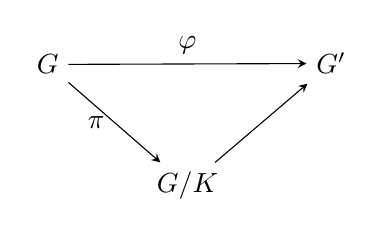
\begin{tikzpicture}
    \node (G) {$G$};
    \node[below right=of G] (GK) {$G/K$};
    \node[above right=of GK] (G') {$G'$};

    \path[->]
      (G)  edge node [above] {$\varphi$}    (G')
      (G)  edge node [left]  {$\pi$}        (GK)
      (GK) edge node [below] {$\varphibar$} (G');
  \end{tikzpicture}
\end{center}

\begin{example}
  If $k : G \to \{ e \}$ is the trivial homomorphism $k(g) = e$ for any $g \in G$, then we get an isomorphism $G/G \cong \{ e \}$ since $\ker(k) = G$.
\end{example}

\begin{example}
  If we consider the identity homomorphism $\id : G \to G$, we get an isomorphism $G/\{ e \} \cong G$ since $\ker(\id) = \{ e \}$.
\end{example}

\begin{example}
  If $\varphi : G \to G'$ is an isomorphism of groups, then the \nameref{claim:fht} recovers this isomorphism since $G \cong G / \{ e \} \cong G'$.
\end{example}

\begin{example}\label{ex:cyclicgroup_homomorphism}
  If $G$ is a group and $g \in G$, we have the familiar group homomorphism $\varphi : \mathbb{Z} \to \braket{g}$ given by $\varphi : k \mapsto g^k$.
  We have shown before that $\varphi$ is surjective.
  Since every subgroup of $\mathbb{Z}$ is of the form $d \mathbb{Z}$ for some $d \in \{ 0, 1, 2, 3, \dots \}$, we have that $\ker(\varphi) = \{ 0 \}$ or $\ker(\varphi) = n \mathbb{Z}$ for some $n \in \mathbb{N}$.
  Furthermore, we verified in Corollary~\ref{cor:isomorphism_iff_homomorphism} that if $\ker(\varphi) = \{ 0 \}$, then $\varphi$ is an isomorphism.
  In the case where $\varphi$ is not injective, say $\ker(\varphi) = n \mathbb{Z}$, we proved that $\braket{g} = \{ e, g, g^2, \dots, g^{n - 1} \}$ and so, by the \nameref{claim:fht}, we conclude that $\mathbb{Z}/n \mathbb{Z} \cong \braket{g}$.
\end{example}

Example~\ref{ex:cyclicgroup_homomorphism} classifies all cyclic groups.
Fix $d \in \{ 0, 1, 2, 3, \dots \}$ and recall that the generalization of Example~\ref{ex:equiv2k} to any $d$ is an equivalence relation.
Also recall from Claim~\ref{claim:subgroups_of_z} that every subgroup of $\mathbb{Z}$ is of the form $d \mathbb{Z}$ for some $d \in \{ 0, 1, 2, 3, \dots \}$.
Since $\mathbb{Z}$ is an abelian group, we have that every such subgroup is normal.
Thus the cosets of any subgroup of $\mathbb{Z}$ are of the form $a + d \mathbb{Z} = \{ a + dk \mid k \in \mathbb{Z} \}$,
and it is clear that the equivalence relation above partitions the group $\mathbb{Z}$ by its cosets.
Let's denote the equivalence class $a + d \mathbb{Z}$ as $\bar{a}$ for any $a \in \mathbb{Z}$.

\begin{claim}
  For $d \geq 1$, there are $d$ distinct elements of the quotient group $\mathbb{Z}/d \mathbb{Z}$ given by $\bar{0}, \bar{1}, \bar{2}, \dots, \bar{d - 1}$.
  That is, $\mathbb{Z}/d \mathbb{Z} = \{ \bar{0}, \bar{1}, \bar{2}, \dots, \bar{d - 1} \}$.

  \begin{proof}
    We can prove this using Example~\ref{ex:cyclicgroup_homomorphism}, noting that $\varphibar(k + d \mathbb{Z}) = \varphi(k) = g^k$ for $0 \leq k \leq d - 1$ whenever $\braket{g} = \{ e, g, g^2, \dots, g^{d - 1} \}$ is a finite cyclic group.

    Alternatively, let $a \in \mathbb{Z}$ and let $b \in \bar{a} = a + d \mathbb{Z}$.
    Then $b = a + kd$ for some $k \in \mathbb{Z}$ and so $b - a = kd$.
    By the \nameref{claim:euclideanalg}, we can write $b = qd + r$ for some integers $q, r$ with $0 \leq r \leq d - 1$.
    Hence $b - r = qd$ as well and thus by transitivity, $r - a = (k - q) d$, or in other words, $r \in \bar{a} = a + d \mathbb{Z}$.
    We conclude that
    \begin{align*}
      \bar{r} &= r + d \mathbb{Z} \\
              &= a + d \mathbb{Z} \\
              &= \bar{a}
    \end{align*}
    with $\bar{r} \in \{ \bar{0}, \bar{1}, \bar{2}, \dots, \bar{d - 1} \}$.
  \end{proof}
\end{claim}

Clearly we have for any $a, b \in \mathbb{Z}$ that
\begin{align*}
  \bar{a} + \bar{b} &= (a + d \mathbb{Z}) + (b + d \mathbb{Z}) \\
                    &= (a + b) + d \mathbb{Z} \\
                    &= \bar{a + b}
\end{align*}
and thus for any $d \geq 1$, we have $\mathbb{Z}/d \mathbb{Z}$ is cyclic of order $d$ generated by $\bar{1}$.
In particular, $\mathbb{Z}/d \mathbb{Z}$ is abelian.

\begin{definition}
  For $n \geq 1$, the quotient group $\mathbb{Z}/n \mathbb{Z}$ is called the group of integers modulo $n$ and is denoted $\mathbb{Z}_n$.
\end{definition}

By Example~\ref{ex:cyclicgroup_homomorphism} we have the following classification:

\begin{corollary}
  All finite cyclic groups of order $n$ are isomorphic to $\mathbb{Z}_n$ while any infinite cyclic group is isomorphic to $\mathbb{Z}$.
\end{corollary}

\section{Rings}
We now begin an investigation of a new kind of algebraic structure that incorporates some familiar friends.

\begin{definition}
  A ring is a set $R$ with two binary operations $+$ and $\cdot$, referred to as addition and multiplication, respectively.
  These operations on $R$ are required to satisfy:
  \begin{enumerate}
    \item $R$ with the operation of addition is an abelian group.
    \item Multiplication is associative; namely for any $r, s, t \in \mathbb{R}$, we have $r \cdot (s \cdot t) = (r \cdot s) \cdot t$.
    \item Multiplication is distributive over addition; namely for any $r, s, t \in R$ we have $r \cdot (s + t) = r \cdot s + r \cdot t$ and $(s + t) \cdot r = s \cdot r + t \cdot r$.
  \end{enumerate}
\end{definition}

We will denote the identity element for the group operation of addition as $0 \in R$.
If the operation of multiplication has an identity element, we will denote it as $1 \in R$.
This multiplicative identity element, when it exists, is sometimes called the unity element of $R$,
and $R$ is said to have unity.
Note that if $1$ and $1'$ are unity elements for $R$, we have the $1 = 1 \cdot 1' = 1'$ and so these elements are unique.

Furthermore, when the operation of multiplication is commutative (i.e. $r \cdot s = s \cdot r$ for any $r, s \in R$), we call $R$ a commutative ring.

\begin{example}
  $\mathbb{R}$ with the usual addition and multiplication of real numbers is a commutative ring with unity.
  These are built into the field axioms defining $\mathbb{R}$ or verified from how $\mathbb{R}$ is constructed from $\mathbb{Q}$.
  \begin{proof} \leavevmode
    \begin{enumerate}
      \item $\mathbb{R}$ with operation $+$ is an abelian group (see Example~\ref{ex:add}).
      \item Multiplication is associative (see Example~\ref{ex:mul}).
      \item For any $x, y, z \in \mathbb{R}$, $x(y + z) = xy + xz$.
        Since $xy = yx$ for any $x, y \in \mathbb{R}$, we also have $(y + z) x = yx + zx$ for any $x, y, z \in \mathbb{R}$.
    \end{enumerate}
    We also noted that the real number 1 has the property $1 \cdot x = x$ for any $x \in \mathbb{R}$.
  \end{proof}
\end{example}

\begin{example}
  $\mathbb{Z}$ is also a commutative ring with unity.
  We have that $\mathbb{Z}$ with our usual operation $+$ is an abelian group and that multiplication is associative.
  Furthermore, for any $p, q, r \in \mathbb{Z}$, we have $p (q + r) = pq + pr$ and since $pq = qp$ for any $p, q \in \mathbb{Z}$, we have the second condition for distributivity that follows immediately.
  As above, we have that $\forall p \in \mathbb{Z}, 1 \cdot p = p$.
\end{example}

\begin{example}
  $\mathbb{Z}_n$ is a commutative ring with unity.
  \begin{proof}
    $\mathbb{Z}_n$ is an abelian group under the group operation $\overline{a} + \overline{b} = \overline{a + b}$.
    Furthermore we an define a multiplication on $\mathbb{Z}_n$ by $\overline{a} \cdot \overline{b} = \overline{ab}$.
    To see that this multiplication is well-defined, notice that if $a \sim a'$ and $b \sim b'$, then $a = a' + kn$ and $b = b' + l n$ for some $k, l \in \mathbb{Z}$. Hence
    \begin{align*}
      ab &= a'b' + a' l n + b' kn + kln^2 \\
         &= a'b' + (a'l + b'k + kln) n \\
         &\sim a' b'
    \end{align*}
    Furthermore, by the \nameref{claim:euclideanalg} we have that $ab = qn + r$ for some $q, r \in \mathbb{Z}$ with $0 \leq r \leq n - 1$ and so
    \begin{align*}
      \overline{a} \cdot \overline{b} &= \overline{ab} \in \{ \overline{0}, \overline{1}, \dots, \overline{n - 1} \} \\
                                      &= \mathbb{Z}_n
    \end{align*}
    To show associativity of $\cdot$, note that for any $\overline{a}, \overline{b}, \overline{c}$, we have
    \begin{align*}
      \overline{a} \cdot (\overline{b} \cdot \overline{c}) &= \overline{a} \cdot (\overline{b c}) \\
                                                           &= \overline{a b c} \\
                                                           &= ( \overline{ab} ) \cdot \overline{c} \\
                                                           &= (\overline{a} \cdot \overline{b}) \cdot \overline{c}
    \end{align*}
    Finally, to show distributivity, note that
    \begin{align*}
      \overline{a} \cdot (\overline{b} + \overline{c}) &= \overline{a} \cdot (\overline{b + c}) \\
                                                       &= \overline{a (b + c)} \\
                                                       &= \overline{ab + ac} \\
                                                       &= \overline{ab} + \overline{ac} \\
                                                       &= \overline{a} \cdot \overline{b} + \overline{a} \cdot \overline{c}
    \end{align*}
    Again, noting that multiplication is commutative since
    \begin{align*}
      \overline{a} \cdot \overline{b} &= \overline{ab} \\
                                      &= \overline{ba} \\
                                      &= \overline{b} \cdot \overline{a}
    \end{align*}
    we can conclude that $(\overline{b} + \overline{c}) \cdot \overline{a} = \overline{b} \cdot \overline{a} + \overline{c} \cdot \overline{a}$ as well.
    Also, as $\overline{1} \cdot \overline{a} = \overline{1a} = \overline{a}$ for any $\overline{a} \in \mathbb{Z}_n$, we have that $\overline{1}$ is the unity element.
  \end{proof}
\end{example}

\begin{example}
  $M_n(\mathbb{R})$ (the set of $n \times n$ matrices with entries in $\mathbb{R}$) was shown to be an abelian group under matrix addition.
  Take the multiplication operation to be the usual multiplication of matrices, which we have argued to be associative before.
  Furthermore, we have from linear algebra that $A \cdot (B + C) = A \cdot B + A \cdot C$ and $(B + C) \cdot A = B \cdot A + C \cdot A$.
  So $M_n(\mathbb{R})$ is a ring, but is not a commutative ring as $M_n(\mathbb{R})$ is not commutative under matrix multiplication.
\end{example}

\subsection{Some Things about Rings}
We can immediately deduce the additive cancellation law, which we proved holds for any group.
In our new additive notation for the group operation $+$, this looks like:

\begin{corollary}
  Let $R$ be a ring and let $a, b, c \in R$.
  If $a + b = a + c$, then $b = c$.
\end{corollary}

Recall that we labeled the identity element of the group $(R, +)$ with 0.
If $a \in R$, then $a$ must have some unique additive inverse with respect to addition.
Keeping with our additive notation for the group operation, label this inverse $-a \in R$.

\begin{corollary}\label{cor:ring_inverses}
  For any $a, b \in R$, we have $a + b = 0$ if and only if $a = -b$ and $b = -a$.
  We also have $- (-a) = a$ and
  \begin{align*}
    -(a + b) &= (-b) + (-a) \\
             &= (-a) + (-b)
  \end{align*}
\end{corollary}

Again, these all follow from results we gathered for groups.
We are just converting our multiplicative notation of an abstract group operation to an additive one.

Here is our first result regarding rings that relies on them being more than abelian groups with addition:

\begin{claim}
  Let $R$ be a ring and let $r, s \in R$ be any elements of $R$.
  Then $r \cdot 0 = 0 \cdot r = 0$ and $(-r) \cdot s = r \cdot (-s) = - (r \cdot s)$.

  \begin{proof}
    For any $r \in R$, we have
    \begin{align*}
      0 + r \cdot 0 &= r \cdot 0 \\
                    &= r \cdot (0 + 0) \\
                    &= r \cdot 0 + r \cdot 0 && \text{by distributivity on the left} \\
      0             &= r \cdot 0             && \text{by the cancellation law}
    \end{align*}
    An identical argument using distributivity on the right and the cancellation law shows $0 \cdot r = 0$.
    For any $r, s \in R$, we have
    \begin{align*}
      r \cdot s + (-r) \cdot s &= (r + -r) \cdot s && \text{by distributivity on the right} \\
                               &= 0 \cdot s \\
                               &= 0
    \end{align*}
    and so $(-r) \cdot s$ is the addition inverse of $r \cdot s$.\footnote{That is, $(-r) \cdot s = -(r \cdot s)$}
    Similarly,
    \begin{align*}
      r \cdot s + r \cdot (-s) &= r \cdot (s + -s) \\
                               &= r \cdot 0 \\
                               &= 0
    \end{align*}
    and so by the uniqueness of inverses, we have $(-r) \cdot s = r \cdot (-s) = -(r \cdot s)$.
  \end{proof}
\end{claim}

It's worth observing that the above claim implies that for any $r, s \in R$ where $R$ is a ring, we have that:
\begin{align*}
  (-r) \cdot (-s) &= -(r \cdot (-s)) \\
                  &= -( -(r \cdot s) ) \\
                  &= r \cdot s && \text{by Corollary~\ref{cor:ring_inverses}}
\end{align*}

We've seen that some rings are special, in that they also have an identity element under the second operation of \enquote{multiplication}.
We labeled this element $1 \in R$ and called it the unity element of $R$.
Is it possible for a ring $R$ with unity to have $1 = 0$ (i.e.\ is it possible for our additive and multiplicative inverses to be the same)?

If $R$ is a ring with unity, and $1 = 0$, then for any $r \in R$, we have that
\begin{align*}
  r &= 1 \cdot r \\
    &= 0 \cdot r \\
    &= 0
\end{align*}
Thus, if $1 = 0$ for any ring $R$ with unity, we have that $R = \{ 0 \}$.
For this reason we will assume henceforth that for any ring with 1, $1 \neq 0$.

It is also worth pointing out why one cannot simply divide by zero.
Let $R$ be a commutative ring with $1$ and let $r \in R$ have a multiplicative inverse $s \in R$ (i.e. $sr = rs = 1$).
We could use a fractional notation $s = \frac{1}{r}$, which would be a good one since $R$ is commutative.
Namely, if $a \in R$ were another element, we would have $a \cdot \frac{1}{r} = \frac{1}{r} \cdot a$, so it would not be dangerous to write either $a \cdot \frac{1}{r}$ or $\frac{1}{r} \cdot a$ as $\frac{a}{r}$.
Moreover, it is always true that $r \cdot \frac{a}{r} = a$ due to commutativity.
Hence, if $0$ had a multiplicative inverse in $R$, we would have that
\begin{align*}
  0 &= 0 \cdot \frac{a}{0} \\
    &= a
\end{align*}
for any $a \in R$.
This implies that $R = \{ 0 \}$ and in particular that $1 = 0$.
The moral is that \enquote{dividing} by 0 is impossible in non-zero commutative rings.

For simplicity, we will write our operation of multiplication $a \cdot b$ in any ring $R$ as $ab$ for any $a, b \in R$.

\section{Domains}
\begin{definition}
  A commutative ring $R$ with 1 is said to be an integral domain (often just \enquote{domain} for short) if the product of any two non-zero elements of $R$ is non-zero.
\end{definition}

\begin{example}
  $\mathbb{Z}$ is an integral domain, since if $p, q \in \mathbb{Z}$ with $p \neq 0$ and $q \neq 0$, then $pq \neq 0$.
  This is where the longer phrase \enquote{integral domain} gets its name.
\end{example}

\begin{example}
  $\mathbb{Z}_6$ is not an integral domain since, for example, $\overline{2} \cdot \overline{3} = \overline{6} = \overline{0}$ where both $\overline{2}$ and $\overline{3}$ are not equal to $\overline{0}$.
\end{example}

\begin{example}\label{ex:zm_composite}
  For the same reason, $\mathbb{Z}_m$ is not an integral domain whenever $m = kl$ for some $k, l \in \mathbb{N}$ with $0 < k, l < m$.
  As above, we have $\overline{k} \cdot \overline{l} = \overline{kl} = \overline{m} = \overline{0}$ where $\overline{k} \neq \overline{0}$ and $\overline{l} \neq \overline{0}$.
\end{example}

Note that the definition of a domain $R$ can be restated by its contrapositive as: whenever $a, b \in R$ with $ab = 0$, then either $a = 0$ or $b = 0$.

\begin{claim}
  A ring $R$ is a domain if and only if it satisfies the multiplicative cancellation law: for any $r, a, b \in R$, if $ra = rb$ and $r \neq 0$,then $a = b$.

  \begin{proof}
    Suppose $R$ is a domain and $ra = rb$ for some $r, a, b \in R$ with $r \neq 0$.
    Then $0 = ra - rb = r(a - b)$.
    But since $r \neq 0$ and $R$ is a domain, we must have that $a - b = 0$, i.e. $a = b$.

    Conversely, suppose $R$ satisfies the multiplicative cancellation law and let $r, a \in R$ with $r \neq 0$.
    Then if $ra = 0$ we have $ra = ra0$, and so $a = 0$ by the cancellation law.
    Thus $R$ is a domain.
  \end{proof}
\end{claim}

The following term should be familiar from linear algebra:

\begin{definition}
  A field $F$ is a commutative ring with 1 in which every non-zero element has a multiplicative inverse (i.e. $\forall r \in F \mid r \neq 0, \exists s \in F \mid rs = sr = 1$).
\end{definition}

Just as we briefly showed that a unity element 1 is unique if a ring $R$ has one,
it is easy to show that multiplicative inverses are unique if they exist.
\begin{proof}
  Let $r \in R$ with $r \neq 0$ have inverses $s, s'$, then
  \begin{align*}
    s &= s1 \\
      &= s (r s') \\
      &= (sr) s' \\
      &= 1 s' \\
      &= s' \qedhere
  \end{align*}
\end{proof}

\begin{example}
  Clearly $\mathbb{R}$ is a field, as we have verified that it is a commutative ring with 1 (the usual real number 1), and has multiplicative inverses ($\forall x \in \mathbb{R} \mid x \neq 0, \exists y = \frac{1}{x} \mid xy = yx = 1$).
\end{example}

\begin{example}
  $\mathbb{C} = \{ a + bi \mid a, b \in \mathbb{R} \}$ is a field.
  \begin{proof}
    There are two natural operations of addition $(a + bi) + (c + di) = (a + c) + (b + d)i$ and multiplication $(a + bi) \cdot (c + di) = (ac - bd) + (ad + bc)i$.
    The addition turns $\mathbb{C}$ into an abelian group (as it is the direct product of $\mathbb{R} \times \mathbb{R}$ with addition), and we have verified that the multiplication defined above is associative.
    That multiplication distributes over addition follows readily from:
    \begin{align*}
      (a + bi) ((c + di) + (e + fi)) &= (a + bi) ((c + e) + (d + f)i) \\
                                     &= (a (c + e) - b(d + f)) + (a (d + f) + b (c + e)) i \\
                                     &= ((ac - bd) + (ae - bf)) + ((ad + bc) + (af + be)) i \\
                                     &= (ac - bd) + (ad + bc)i + (ae - bf) + (af + be)i \\
                                     &= (a + bi) (c + di) + (a + bi) (e + fi)
    \end{align*}
    for any $(a + bi), (c + di), (e + fi) \in \mathbb{C}$.
    Additionally, it is routine to check that multiplication is commutative since
    \begin{align*}
      (a + bi)(c + di) &= (ac - bd) + (ad + bc)i \\
                       &= (ca - db) + (da + cb)i \\
                       &= (c + di) (a + bi)
    \end{align*}
    for any $(a + bi), (c + di) \in \mathbb{C}$.
    Finally, we know that $1 = 1 + 0i$ is the unity element, and that every non-zero complex number has an inverse under multiplication.
    So $\mathbb{C}$ is a field.
  \end{proof}
\end{example}

\begin{example}
  $\mathbb{Z}$ is definitely not a field as only $\{ 1, -1 \}$ have multiplicative inverses in $\mathbb{Z}$.
\end{example}

\begin{example}
  $\mathbb{Q} \subset \mathbb{R}$ is also a field.
  It is easy to verify from the usual definition of addition and multiplication of rational numbers (to be done later).
\end{example}

It is clear that not every domain is a field (with $\mathbb{Z}$ as an example).
Nevertheless, we might want to know if every field is a domain.
The answer is yes and the proof is quick.

\begin{claim}
  Every field is an integral domain.

  \begin{proof}
    Let $R$ be a field.
    Then $R$ is a commutative ring with 1.
    By the above, we need only demonstrate that $R$ satisfies the multiplicative cancellation property to show that $R$ is a domain.
    Let $r, a, b \in R$ with $r \neq 0$ and suppose that $ra = rb$.
    Since $R$ is a field, there exists an inverse $s \in R$ of $r$.
    Then
    \begin{align*}
      a &= 1a \\
        &= (sr) a \\
        &= s (ra) \\
        &= s (rb) \\
        &= (sr) b \\
        &= 1b \\
        &= b
    \end{align*}
    Hence $R$ satisfies the cancellation property and is thus a domain.
  \end{proof}
\end{claim}

We have the now famous fact that every nontrivial subgroup of $(\mathbb{Z}, +)$ is of the form $d \mathbb{Z}$ for some $d \in \mathbb{N}$.
Fix integers $a, b \in \mathbb{Z}$, not both zero, and define a subset of $a \mathbb{Z} + b \mathbb{Z} = \{ ka + lb \mid k, l \in \mathbb{Z} \}$.
It's quick to check that $a \mathbb{Z} + b \mathbb{Z}$ is a subgroup of $\mathbb{Z}$.
Hence $a \mathbb{Z} + b \mathbb{Z} = d \mathbb{Z}$ for some $d \geq 1$.
This number $d$ is called the greatest common divisor of $a$ and $b$.

This natural number $d$ divides both $a$ and $b$, and any other natural number dividing both $a, b$ necessarily divides $d$.
Let's verify both of these: $d$ divides $a$ since $a = 1a + 0b \in a \mathbb{Z} + b \mathbb{Z}$ and so $a = pd$ for some $p \in \mathbb{Z}$; similarly $b = 0a + 1b = qd$ for some $q \in \mathbb{Z}$.
Furthermore, if $m \in \mathbb{N}$ divides $a$ and $b$ (i.e. $a = pm$ and $b = qm$ for some $p, q \in \mathbb{Z}$), then for some $k, l \in \mathbb{Z}$ we have
\begin{align*}
  d &= ka + lb && \text{since $d \in d \mathbb{Z} = a \mathbb{Z} + b \mathbb{Z}$} \\
    &= k (pm) + l (qm) \\
    &= (kp + lq) m
\end{align*}
so $m$ divides $d$.

Besides reducing some elementary number theory to group theory, the previous discussion is useful for the following curious ring-theoretic result:

\begin{claim}\label{claim:zn_field}
  If $p \in \mathbb{N}$ is prime, then $\mathbb{Z}_p$ is a field.

  \begin{proof}
    Clearly the unity element $\overline{1}$ is invertible and $\overline{p} = \overline{0}$ is not.
    So let $a \in \mathbb{Z}$ with $1 < a < p$ and consider $\overline{a} \in \mathbb{Z}_p$.
    The hypothesis \enquote{$p$ is prime} implies that for any $a$, the greatest common divisor of $p$ and $a$ is $d = 1$.
    Hence for some $k, l \in \mathbb{Z}$,
    \begin{align*}
      1      &= d \\
             &= ka + lp \\
      1 - ka &= lp
    \end{align*}
    Thus $1 \sim ka \pmod{p}$ and we have $\overline{k} \cdot \overline{a} = \overline{ka} = \overline{1}$.
    We conclude that $\overline{a}$ is invertible.
    Since $\overline{a}$ is arbitrary non-unity, non-zero element of $\mathbb{Z}_p$, we have that $\mathbb{Z}_p$ is a field.
  \end{proof}
\end{claim}

Why is this curious?
We showed in Example~\ref{ex:zm_composite} that $\mathbb{Z}_n$ is not even an integral domain if $n$ is not prime.
However, we just showed in Claim~\ref{claim:zn_field} that if $n$ is prime, then $\mathbb{Z}_n$ is not only an integral domain, but a field.
These finite rings do not have much variability in this regard: they either fail to be domains or every non-zero element has a multiplicative inverse.

\subsection{Subrings and Ring Homomorphisms}
\begin{definition}\label{def:subring}
  A subring of a ring $R$ is a subset $S \subseteq R$ that is:
  \begin{enumerate}
    \item closed under subtraction, i.e. $r - s \in S$ for any $r, s \in S$
    \item closed under multiplication, i.e. $rs \in S$ for any $r, s \in S$
  \end{enumerate}
\end{definition}

It is easy to verify that subrings are rings in their own right (see first two pages of \emph{Ideals and Homomorphisms} in Pinter).

\begin{example}\label{ex:subring_self}
  Clearly, every ring $R$ is a subring of itself.
\end{example}

\begin{example}\label{ex:subring_zero}
  If $R$ is a ring, then $\{ 0 \}$ is a subring of $R$.
\end{example}

\begin{example}\label{ex:subring_Z}
  $\mathbb{Z}$ is a subring of $\mathbb{Q}$.
\end{example}

\begin{example}\label{ex:subring_Q}
  $\mathbb{Q}$ is a subring of $\mathbb{R}$.
\end{example}

\begin{example}\label{ex:subring_R}
  $\mathbb{R}$ is a subring of $\mathbb{C}$.
\end{example}

\begin{example}\label{ex:subring_nZ}
  $n \mathbb{Z}$ is a subring of $\mathbb{Z}$ for any $n \in \{ 0, 1, 2, \dots \}$.
\end{example}

\begin{comment}
  In most algebra textbooks, rings are taken to be commutative rings with unity and subrings are required to contain the unity element.
  Note that Examples~\ref{ex:subring_self},~\ref{ex:subring_Z},~\ref{ex:subring_Q}, and~\ref{ex:subring_R} are subrings in this more restrictive sense,
  but Examples~\ref{ex:subring_zero} and~\ref{ex:subring_nZ} are not.
\end{comment}

\begin{definition}
  If $R$ and $R'$ are rings, then a function $\varphi : R \to R'$ is called a ring homomorphism if for all $r, s \in R$, we have:
  \begin{displaymath}
    \begin{gathered}
      \varphi(\underbrace{r + s}_\text{in $R$}) = \underbrace{\varphi(r) + \varphi(s)}_\text{in $R'$}
    \end{gathered}
    \qquad \text{and} \qquad
    \begin{gathered}
      \varphi(\underbrace{r \cdot s}_\text{in $R$}) = \underbrace{\varphi(r) \cdot \varphi(s)}_\text{in $R'$}
    \end{gathered}
  \end{displaymath}
\end{definition}

Clearly, the first requirement of a ring homomorphism $\varphi : R \to R'$ is that it be a group homomorphism from $(R, +)$ to $(R', +)$.

\begin{definition}
  A ring homomorphism $\varphi : R \to R'$ is an isomorphism if $\varphi$ is a bijection.
  In this case, we say $R$ and $R'$ are isomorphic and write $R \cong R'$.
\end{definition}

\begin{example}
  The identity function $\id : R \to R$ defined by $\id(r) = r$ for any $r \in R$ is a ring homomorphism.
\end{example}

\begin{example}
  The function $k : R \to \{ 0 \}$ defined by $k(r) = 0$ for any $r \in R$ is a ring homomorphism.
\end{example}

\begin{example}
  If $S$ is a subring of $R$, the inclusion $\iota : S \to R$ defined by $\iota(s) = s$ for any $s \in S$ is a ring homomorphism.
\end{example}

\begin{example}
  The function $\pi : \mathbb{Z} \to \mathbb{Z}_n$ defined by $\pi(a) = \overline{a}$ for any $a \in \mathbb{Z}$ is a surjective ring homomorphism.
  We have from Claim~\ref{claim:canonicalmap_homomorphism} that it is a group homomorphism.
  It is a ring homomorphism since
  \begin{align*}
    \pi(ab) &= \overline{ab} \\
            &= \overline{a} \cdot \overline{b} \\
            &= \pi(a) \cdot \pi(b)
  \end{align*}
\end{example}

\begin{definition}
  If $\varphi : R \to R'$ is a ring homomorphism, then its kernel is the set $\ker(\varphi) = \{ r \in R \mid \varphi(r) = 0' \in R' \}$ where $0'$ is the zero element in $R'$.
  Similarly, the image of $\varphi$ is the set $\ima(\varphi) = \{ r' \in R' \mid r' = \varphi(r) \text{ for some } r \in R \}$.
\end{definition}

Just as the kernel of a group homomorphism is a special kind of subgroup of the domain (a normal subgroup), kernels of ring homomorphisms are special kinds of subrings of the domain.

\begin{definition}
  An ideal of a ring $R$ is a subset $I \subseteq R$ such that
  \begin{enumerate}
    \item $I$ is closed under subtraction
    \item $I$ absorbs products; that is, for any $a \in I$ and $r \in R$, we have $ra \in I$ and $ar \in I$.
  \end{enumerate}
  If $I \neq R$, then $I$ is said to be a proper ideal of $R$.
\end{definition}

Notice that in our above definition of an ideal $I$ of a ring $R$, we have that $0 \in R$ must be an element of $I$ (just like in the \hyperref[def:subring]{definition of a subring}).
This follows at once from $I$ being closed under subtraction, which you showed for homework is equivalent to $I$ being a subgroup of $R$ under addition.

Furthermore, if $R$ is a commutative ring and $I$ is a subgroup of $R$ under addition, we need only check that for any $r \in R$ and any $a \in I$, $ra \in I$ to show $I$ is an ideal of $R$.
Commutativity of multiplication saves us from having to show that $ar \in I$ as well.

\begin{example}
  $R$ is an ideal of $R$.
\end{example}

\begin{example}
  $\{ 0 \}$ is an ideal of $R$.
\end{example}

\begin{example}
  If $\varphi : R \to R'$ is a ring homomorphism, then $\ker(\varphi)$ is an ideal of $R$.

  \begin{proof}
    Since $\varphi$ is a ring homomorphism, it is a group homomorphism from $(R, +)$ to $(R', +)$ and so clearly $\ker(\varphi)$ is a subgroup of $(R, +)$.
    Hence, if $a, b \in \ker(\varphi)$, then $a - b \in \ker(\varphi)$.
    Furthermore, if $r \in R$ and $a \in \ker(\varphi)$, then
    \begin{align*}
      \varphi(ra) &= \varphi(r) \varphi(a) \\
                  &= \varphi(r) \cdot 0' \\
                  &= 0'
    \end{align*}
    where $0'$ is the zero element in $R'$.
    Hence, $\varphi(ra) = 0'$, so $ra \in \ker(\varphi)$.
  \end{proof}
\end{example}

\begin{example}
  Let $n \in \mathbb{Z}$ and define $(n) = n \mathbb{Z} \subseteq \mathbb{Z}$.
  Then $(n)$ is the ideal of $\mathbb{Z}$ consisting of all multiples of $n$.
\end{example}
This is a special case of a more general construction:

\begin{example}
  Let $R$ be a commutative ring with 1.
  If $a \in R$, the set $(a) = \{ s \in R \mid s = ra \text{ for some } r \in R \}$ is an ideal in $R$ called the principal ideal generated by $a$.

  \begin{proof}
    Evidently, $(a)$ is a subset of $R$.
    If $s \in (a)$, then $s = r' a$ for some $r' \in R$ and so for any $r \in R$, we have
    \begin{align*}
      rs &= r (r' a) \\
         &= (r r') a \\
         &\in (a) && \text{since $rr' \in R$}
    \end{align*}
    so $(a)$ absorbs products.
    Furthermore, if $s, t \in (a)$, then $s = ra$ and $t = r' a$ for some $r, r' \in R$.
    Thus
    \begin{align*}
      s - t &= ra - r' a \\
            &= (r - r') a \\
            &\in (a) && \text{since $r - r' \in R$}
    \end{align*}
    and so $(a)$ is closed under subtraction.
  \end{proof}
\end{example}

In general, the image of a ring homomorphism $\varphi : R \to R'$ is not an ideal of $R'$ unless $\varphi$ is surjective.
However, it is always a subring of $R'$ as you will show for homework.

\subsection{Quotient Rings}

Let $I$ be an ideal of a ring $R$.
As we've seen, forgetting about multiplication in $R$ we have that $I$ with addition is a subgroup of $(R, +)$.
Since $R$ with addition is an abelian group, we have that $I$ must be a normal subgroup of $R$.
Hence the quotient group $R/I$ exists.

Its elements are the cosets $r + I$ where $r \in R$ with addition on $R/I$ defined by
\begin{displaymath}
  (r + I) + (r' + I) = (r + r') + I
\end{displaymath}.
In particular, this addition is commutative, and the additive identity (zero element) is $0 + I = I$.
Furthermore, $r + I = r' + I$ if and only if $r - r' \in I$, and we have that the canonical (natural) map $\pi : R \to R/I$ defined by $\pi(r) = r + I$ is a surjective group homomorphism.

So far, everything we said would be true if $I$ was an arbitrary subring of $R$, but the following would not:

\begin{claim}\label{claim:abelianmult_ring}
  Let $I$ be a proper ideal in a ring $R$.
  Then the additive abelian group $R/I$ can be equipped with a multiplication making it into a ring, and making the canonical map $\pi : R \to R/I$ into a surjective ring homomorphism.

  \begin{proof}
    Define multiplication on $R/I$ by $(r + I) \cdot (r' + I) = rr' + I$, where $r, r' \in R$.
    This is well defined, since if $r + I = s + I$ and $r' + I = s' + I$ for any $r, r', s, s' \in R$, then $rr' + I = ss' + I$.
    To see, this, note that
    \begin{align*}
      rr' - ss' &= (rr' - rs') + (rs' - ss') \\
                &= r (\underbrace{r' - s'}_{\in I}) + (\underbrace{r - s}_{\in I}) s' && \text{by our hypothesis} \\
                &= \underbrace{r (r' - s')}_{\in I} + \underbrace{(r - s) s'}_{\in I} && \text{since $I$ absorbs products} \\
                &\in I
    \end{align*}
    which means $rr' + I = ss' + I$.

    We already have (from the above group theory) that $R/I$ is an abelian group under addition of cosets $(r + I) + (r' + I) = (r + r') + I$,
    so we only need to show that our multiplication is associative and distributes over addition.
    To see that the above multiplication is associative, we have for any $r, r', r'' \in R$:
    \begin{align*}
      \left( (r + I) \cdot (r' + I) \right) \cdot (r'' + I) &= (rr' + I) \cdot (r'' + I) \\
                                                            &= (rr') r'' + I \\
                                                            &= r (r' r'') + I \\
                                                            &= (r + I) \cdot (r r'' + I) \\
                                                            &= (r + I) \cdot \left( (r' + I) \cdot (r'' + I) \right)
    \end{align*}
    For homework, you will show that multiplication distributes over addition.

    Finally, we know that the canonical map $\pi : R \to R/I$ is a surjective group homomorphism and since
    \begin{align*}
      \pi(r r') &= r r' + I \\
                &= (r + I) \cdot (r' + I) \\
                &= \pi(r) \cdot \pi(r')
    \end{align*}
    we have that $\pi$ is a surjective ring homomorphism.
  \end{proof}
\end{claim}

\begin{definition}
  If $R$ is a ring, and $I$ is an ideal of $R$, the ring $R/I$ outfitted with the multiplication in Claim~\ref{claim:abelianmult_ring} is called the quotient ring of $R$ by $I$, or the quotient ring of $R$ modulo $I$.
\end{definition}

\begin{example}
  $\mathbb{Z}/(n) = \mathbb{Z}/n \mathbb{Z} = \mathbb{Z}_n$ is the quotient ring of $\mathbb{Z}$ modulo $(n)$.
  Just as in the group theory setting, the canonical map $\pi : \mathbb{Z} \to \mathbb{Z}_n$ defined by $\pi(n) = \overline{n}$ for any $n \in \mathbb{Z}$ has kernel $\ker(\pi) = n \mathbb{Z} = (n)$.
  In fact, there's really nothing new going on here except that our definition of multiplication of cosets turns this group homomorphism $\pi$ into a ring homomorphism.
  Actually, this is exactly the reason we defined multiplication in $\mathbb{Z}_n$ this way.
\end{example}

\subsection{The Fundamental Homomorphism Theorem for Rings}

\begin{claim}[Fundamental Homomorphism Theorem for Rings]
  If $\varphi : R \to R'$ is a surjective ring homomorphism with $\ker(\varphi) = I$, then $R/I \cong R'$.

  \begin{proof}
    Again forgetting multiplication in $R$ and $R'$ and looking at both just as groups under addition,
    we have that the function $\overline{\varphi} : R/I \to R'$ defined by $\overline{\varphi}(r + I) = \varphi(r)$ is a group isomorphism.
    It is also a ring homomorphism since
    \begin{align*}
      \overline{\varphi} \left( (r + I) \cdot (s + I) \right) &= \overline{\varphi}(rs + I) \\
                                                              &= \varphi(rs) \\
                                                              &= \varphi(r) \varphi(s) \\
                                                              &= \overline{\varphi}(r + I) \overline{\varphi}(s + I) \\
    \end{align*}
    Thus $\varphi : R/I \to R'$ is a ring homomorphism.
  \end{proof}
\end{claim}

\begin{claim}
  A commutative ring $R$ with 1, is a field if and only if there is only one proper ideal of $R$, the zero ideal.

  \begin{proof}
    If $R$ is a field and $I \subseteq R$ then $R \neq I$ and $I$ absorbs products.
    Suppose for contradiction that $I \neq \{ 0 \}$.
    Then there is some $s \neq 0$ in $I$.
    But since $R$ is a field, we have that $\frac{1}{s} \in R$ and so $\frac{1}{s} s = 1 \in I$ as $I$ absorbs products.
    Hence for any $r \in R$ we have that $r1 = r \in I$ and so $R = I$ contradicting $R \neq I$.

    Conversely, suppose that the only proper ideal $I$ of $R$ is the zero ideal $I = \{ 0 \}$.
    Let $r \neq 0$ and consider the principal ideal $(r)$ generated by $r$.
    By hypothesis we must have $(r) = R$, otherwise this would be a non-zero proper ideal of $R$.
    Since $1 \in R$ there must be some $s \in R$ so that $sr = 1$, i.e. $r$ has a multiplicative inverse.
    Since $r$ is an arbitrary non-zero element, we have that $R$ is a field.
  \end{proof}
\end{claim}

\begin{claim}
  Every finite integral domain is a field.

  \begin{proof}
    Suppose $R$ is a finite integral domain.
    Then $R = \{ 0, 1, r_1, r_2, \dots, r_n \}$ where each $r_j$ is distinct and not 0 or 1.
    Fix $j = 1, \dots, n$ and consider the set $r_j R = \{ 0, r_j, r_j r_1, \dots, r_j r_n \}$ obtained by multiplying every element of $R$ by $r_j$.
    Since $R$ is an integral domain we have that $r_j r = r_j s$ if and only if $r = s$ for any $r, s \in R$.
    In particular, $R$ and $r_j R$ have the same cardinality.
    But then $r_j R = R$ and so for some $r_k \in R$ we must have $r_j r_k = 1$.
    Since $j = 1, \dots, n$ is arbitrary, we have that every non-zero element of $R$ has a multiplicative inverse.
  \end{proof}
\end{claim}

\section{Characteristic}

Commutative rings with unity have the characteristic, a number associated with them,
giving us information as to how addition interacts with the multiplicative identity.

\begin{definition}
  Let $R$ be a commutative ring with 1.
  We say $R$ has characteristic $n$ if
  \begin{displaymath}
    \underbrace{1 + 1 + \cdots + 1}_\text{$n$ times} = 0 \qquad\text{for some least $n \in \mathbb{N}$}
  \end{displaymath}
  If no such $n \in \mathbb{N}$ exists, we say that $R$ has characteristic 0.
\end{definition}

\begin{claim}
  If $R$ is an integral domain of characteristic $n \geq 1$, then all non-zero elements of $R$ have the same additive order.

  \begin{proof}
    Let $r \in R$ with $r \neq 0$.
    \begin{displaymath}
      \underbrace{r + r + \cdots + r}_\text{$n$ times} = r (\underbrace{1 + 1 + \cdots + 1}_\text{$n$ times}) = 0
    \end{displaymath}
    That is, the additive order of any non-zero element is the characteristic of $R$.
  \end{proof}
\end{claim}

\begin{claim}
  If $R$ is an integral domain with non-zero characteristic $n$, then $n$ is prime.

  \begin{proof}
    The proof is by contrapositive.
    Suppose that $n$ is not prime, so $n = kl$ for some $k, l \in \mathbb{N}$ with $1 < k, l < n$.
    Then
    \begin{align*}
      0 = \underbrace{1 + 1 + \cdots + 1}_\text{$n$ times} = (\underbrace{1 + 1 + \cdots + 1}_\text{$k$ times, $\neq 0$}) \cdot (\underbrace{1 + 1 + \cdots + 1}_\text{$l$ times, $\neq 0$})
    \end{align*}
    since $n$ is the least natural number so that $\underbrace{1 + 1 + \cdots + 1}_\text{$n$ times} = 0$.
    But their product is 0, hence $R$ is not an integral domain.
  \end{proof}
\end{claim}

The following mostly has nothing to do with abstract algebra (the argument is in chapter 20 of Pinter):
\begin{lemma}
  If $p \in \mathbb{N}$ is prime, then $p$ divides $\binom{p}{k}$ for any $0 < k < p$.
\end{lemma}

\begin{definition}
  Let $R$ be a commutative ring with 1.
  For any $r \in R$, label $\underbrace{r + r + \cdots + r}_\text{$k$ times}$ as $kr$ and label $\underbrace{r \cdot r \cdots r \cdot r}_\text{$r$ times}$ as $r^k$ for any $k \in \mathbb{Z}$.
\end{definition}

In the above definition, we take $0r = 0 \in R$ and $r^0 = 1 \in R$ where the 0 on the left-hand side of both equalities is the usual $0 \in \mathbb{Z}$.

\begin{claim}
  In any integral domain $R$ of characteristic $p$, we have that ${(a + b)}^p = a^p + b^p$ for all $a, b \in R$.

  \begin{proof}
    We have by the binomial theorem that
    \begin{align*}
      {(a + b)}^p &= \sum_{k = 0}^p \binom{p}{k} a^k b^{p - k} \\
                  &= a^p + \sum_{k = 1}^{p - 1} \binom{p}{k} a^k b^{p - k} + b^p \\
                  &= a^p + 0 + b^p \\
                  &= a^p + b^p
    \end{align*}
    where $\sum_{k = 1}^{p - 1} \binom{p}{k} a^k b^{p - k} = 0$ since $R$ has characteristic $p$ and $\binom{p}{k}$ is a multiple of $p$ for any natural number $k$ satisfying $1 \leq k \leq p - 1$.
  \end{proof}
\end{claim}

\subsection{The Field of Fractions of an Integral Domain}

Every field is an integral domain, but the converse is obviously false as $\mathbb{Z}$ is an integral domain that is not a field.
However, the next claim shows that every integral domain can be extended to a field in the same way that $\mathbb{Z}$ is extended to $\mathbb{Q}$:

\begin{claim}
  If $R$ is an integral domain, then there is a unique field $F$ called the field of fractions of $R$ that contains an isomorphic copy of $R$ as a subring.
  We denote this field by $F = \Frac(R)$.

  \begin{proof}
    Given an integral domain $R$, define the set $\Frac(R)$ as follows:
    consider the subset $S$ of the Cartesian product $R \times R = \{ (a, b) \mid a, b \in R \}$ defined by $S = \{ (a, b) \in R \times R \mid b \neq 0 \}$.

    We define the equivalence relation of \enquote{cross multiplication} on $S$ by $(a, b) \sim (c, d)$ if $ad = bc$ in $R$.
    After checking that this is in fact an equivalence relation, we define $\Frac(R)$ to be the set of equivalence classes of this equivalence relation on $S$.

    Let's check that cross multiplication is an equivalence relation.
    If $(a, b) \sim (c, d)$ and $(c, d) \sim (e, f)$, then $ad = bc$ and $cf = de$.
    Hence
    \begin{align*}
      adcf &= bcde \\
      dc(af) &= dc(be) && \text{by commutativity of $R$}
    \end{align*}
    Since $R$ is an integral domain, we have that $af = be$, and so $(a, b) \sim (e, f)$; thus the relation in transitive.
    If $(a, b) \sim (c, d)$, then
    \begin{align*}
      ad &= bc \\
      cb &= da && \text{also by commutativity}
    \end{align*}
    which implies $(c, d) \sim (a, b)$, so the relation is symmetric.
    That the relation is reflexive follows again from commutativity, i.e. $ab = ba$, and so $(a, b) \sim (a, b)$.

    As anticipated, we let $\Frac(R)$ be the set of equivalence classes of this relation on $S$ and denote the equivalences classes $[(a, b)]$ by $\frac{a}{b}$.
    So
    \begin{displaymath}
      \Frac(R) = \left\{ \frac{a}{b} \mid a, b \in R \text{ with } b \neq 0 \right\}
    \end{displaymath}

    We now introduce the two familiar operations of addition and multiplication on $\Frac(R)$ by
    \begin{align*}
      \frac{a}{b} + \frac{c}{d} = \frac{ad + bc}{bd} \qquad \text{and} \qquad \frac{a}{b} \cdot \frac{c}{d} = \frac{ac}{bd} \qquad \text{for any $\frac{a}{b}, \frac{c}{d} \in \Frac(R)$}
    \end{align*}
    Let's check that these operations are well-defined:
    in both cases, $bd \neq 0$ as by hypothesis $b \neq 0$ and $d \neq 0$, and using that $R$ is an integral domain.
    To check that these are operations at all, we need to make sure that the above definitions of addition and multiplication of fractions don't depend on a choice of representatives of the equivalence classes $[(a, b)] = \frac{a}{b}$.

    To this end, let $\frac{a}{b} = \frac{a'}{b'}$ and $\frac{c}{d} = \frac{c'}{d'}$, so $ab' = ba'$ and $cd' = dc'$.
    We have $\frac{a}{b} + \frac{c}{d} = \frac{ad + bc}{bd}$ and $\frac{a'}{b'} + \frac{c'}{d'} = \frac{a'd' + b'c'}{b'd'}$.
    Notice that:
    \begin{align*}
      (ad + bc) (b' d') &= (a d) (b' d') + (b c) (b' d') \\
                        &= (a b') (d d') + (c d') (b b') \\
                        &= (b a') (d d') + (d c') (b b') \\
                        &= (a' d') (b d) + (b' c') (b d) \\
                        &= (a' d' + b' c') (b d)
    \end{align*}
    and so $(ad + bc, bd) \sim (a' d' + b' c', b' d')$; or in other words, $\frac{ad + bc}{bd} = \frac{a' d' + b' c'}{b' d'}$.
    Similarly, since
    \begin{align*}
      (a' c') (b d) &= (a' b) (c' d) \\
                    &= (b' a) (c d') \\
                    &= (a c) (b' d')
    \end{align*}
    we have $\frac{a' c'}{b' d'} = \frac{ac}{bd}$ and so both addition and multiplication are, in fact, well-defined operations.

    Now that we can safely use these operations, we need to check that they turn $\Frac(R)$ into a field.
    You will show for homework that addition and multiplication are both associative and commutative, and that multiplication distributes over addition.

    Let $\frac{a}{b} \in \Frac(R)$.
    The element $\frac{0}{1}$ is the zero element in $\Frac(R)$ since we have that
    \begin{displaymath}
      \frac{a}{b} + \frac{0}{1} = \frac{a1 + b0}{b1} = \frac{a}{b}
    \end{displaymath}
    Furthermore, $\frac{0}{r} = \frac{0}{1}$ for any $r \neq 0 \in R$ since $01 = r0$.
    The additive inverse of any element $\frac{a}{b}$ is $\frac{-a}{b}$ as
    \begin{displaymath}
      \frac{a}{b} + \frac{-a}{b} = \frac{ab - ba}{b^2} = \frac{0}{b^2} = \frac{0}{1}
    \end{displaymath}
    Lastly, $\frac{1}{1}$ is the unity element as
    \begin{displaymath}
      \frac{a}{b} \cdot \frac{1}{1} = \frac{a1}{b1} = \frac{a}{b}
    \end{displaymath}
    and every element has a multiplicative inverse since if $\frac{a}{b} \neq \frac{0}{1}$, then
    \begin{align*}
      a1 &\neq b0 \\
      a &\neq 0
    \end{align*}
    and so
    \begin{displaymath}
      \frac{b}{a} \in \Frac(R) \qquad \text{with} \qquad \frac{a}{b} \cdot \frac{b}{a} = \frac{ab}{ba} = \frac{1}{1}
    \end{displaymath}

    To finish the claim, define the function $\varphi : R \to \Frac(R)$ by $\varphi(r) = \frac{r}{1}$ for any $r \in R$.
    The function $\varphi$ is a ring homomorphism as
    \begin{displaymath}
      \varphi(r + s) = \frac{r + s}{1} = \frac{r1 + 1s}{1} = \frac{r}{1} + \frac{s}{1} = \varphi(r) + \varphi(s)
    \end{displaymath}
    This ring homomorphism is injective since if $\varphi(r) = \frac{r}{1} = \frac{0}{1}$, then we can conclude that
    \begin{align*}
      r &= r1 \\
        &= 1 \cdot 0 \\
        &= 0
    \end{align*}
    , so $\ker(\varphi) = \{ 0 \}$.
    The image of a ring homomorphism is always a subring of the codomain, so
    \begin{displaymath}
      \ima(\varphi) = \left\{ \frac{r}{1} \in \Frac(R) \mid r \in R \right\}
    \end{displaymath}
    is a subring of $\Frac(R)$ that is isomorphic to $R$.
  \end{proof}
\end{claim}

It is maybe worth going through the above argument for $R = \mathbb{Z}$ and observing that all of these abstract constructions are merely generalizations of the natural way of getting $\mathbb{Q}$ out of $\mathbb{Z}$.

\begin{definition}\label{def:poly}
  If $R$ is a commutative ring with 1, then we define a polynomial $f(x)$ with coefficients in $R$, or \enquote{a polynomial over $R$}, to be a sequence $f(x) = (a_0, a_1, a_2, \dots, a_n, 0, 0, \dots)$ with $a_j \in R$ for each $j \leq 0$ and $a_j = 0$ for all $j > n$.
  If $g(x) = (b_0, b_1, \dots, b_m, 0, 0, \dots)$ is another polynomial over $R$, we say that $g(x) = f(x)$ when $a_j = b_j$ for all $j \geq 0$.
  We denote the set of polynomials over $R$ by $R[x]$.
  This is just the set of sequences with terms in the ring $R$ that are eventually zero.
\end{definition}

\begin{definition}
  Let $R[x]$ be the set of polynomials over the commutative ring $R$.
  We can define an addition and a multiplication on $R[x]$.
  For any $f(x) = (a_0, a_1, a_2, \dots, a_n, 0, 0, \dots)$ and $g(x) = (b_0, b_1, \dots, b_m, 0, 0, \dots)$ as above, we let
  \begin{equation}\label{def:poly_add}
    f(x) + g(x) = (a_0 + b_0, a_1 + b_1, a_2 + b_2, \dots)
  \end{equation}
  Multiplication of polynomials is defined by
  \begin{equation}\label{def:poly_mul}
    f(x) \cdot g(x) = (m_0, m_1, m_2, \dots) \qquad \text{where $m_j = \sum_{r + s = j} a_r b_s$ for $j \geq 0$}
  \end{equation}
\end{definition}

For example, writing the first few terms of the product we have:
\begin{displaymath}
  f(x) \cdot g(x) = (a_0 b_0, a_0 b_1 + a_1 b_0, a_0 b_2 + a_1 b_1 + a_2 b_0, a_0 b_3 + a_1 b_2 + a_2 b_1 + a_3 b_0, \dots)
\end{displaymath}

\begin{claim}\label{claim:commutativering_rx}
  Let $R$ be a commutative ring with unity.
  With the addition and multiplication defined in Equations~\ref{def:poly_add} and~\ref{def:poly_mul}, $R[x]$ (the set of polynomials over $R$) is a commutative ring with unity.

  \begin{proof}
    For notational convenience, let $\boldsymbol( a_j \boldsymbol)$ denote any sequence $(a_0, a_1, a_2, a_3, \dots)$.
    The operation of $+$ is commutative since if $f(x), g(x) \in R[x]$ are polynomials, we have that $f(x) = \boldsymbol( a_j \boldsymbol)$ and $g(x) = \boldsymbol( b_j \boldsymbol)$ for some eventually zero sequences $\boldsymbol( a_j \boldsymbol), \boldsymbol( b_j \boldsymbol)$.
    Then
    \begin{align*}
      f(x) + g(x) &= \boldsymbol( a_j \boldsymbol) + \boldsymbol( b_j \boldsymbol) \\
                  &= \boldsymbol( a_j + b_j \boldsymbol) \\
                  &= \boldsymbol( b_j + a_j \boldsymbol) \\
                  &= \boldsymbol( b_j \boldsymbol) + \boldsymbol( a_j \boldsymbol) \\
                  &= g(x) + f(x)
    \end{align*}
    We have that the polynomial $0(x) = (0, 0, 0, \dots) = \boldsymbol( 0 \boldsymbol)$ is the zero element in $R[x]$ since
    \begin{align*}
      f(x) + 0(x) &= \boldsymbol( a_j \boldsymbol) + \boldsymbol( 0 \boldsymbol) \\
                  &= \boldsymbol( a_j + 0 \boldsymbol) \\
                  &= \boldsymbol( a_j \boldsymbol) \\
                  &= f(x)
    \end{align*}
    Let $h(x) = \boldsymbol( c_j \boldsymbol)$ be a third polynomial in $R[x]$.
    The operation $+$ is associative since
    \begin{align*}
      \left( \boldsymbol( a_j \boldsymbol) + \boldsymbol( b_j \boldsymbol) \right) + \boldsymbol( c_j \boldsymbol) &= \boldsymbol( a_j + b_j \boldsymbol) + \boldsymbol( c_j \boldsymbol) \\
                                                                                                                   &= \boldsymbol( a_j + b_j + c_j \boldsymbol) \\
                                                                                                                   &= \boldsymbol( a_j \boldsymbol) + \boldsymbol( b_j + c_j \boldsymbol) \\
                                                                                                                   &= \boldsymbol( a_j \boldsymbol) + \left( \boldsymbol( b_j \boldsymbol) + \boldsymbol( c_j \boldsymbol) \right) \\
    \end{align*}
    Multiplication is also associative since
    \begin{align*}
      \boldsymbol( a_j \boldsymbol) + \left( \boldsymbol( b_j \boldsymbol) \boldsymbol( c_j \boldsymbol) \right) &= \boldsymbol( a_j \boldsymbol) \boldsymbol( \sum_{i + k = j} b_i c_k \boldsymbol) \\
                                                                                                                 &= \left( \sum_{r + s = j} a_r \left( \sum_{i + k = s} b_i c_k \right) \right) \\
                                                                                                                 &= \left( \sum_{r + i + k = j} a_r b_i c_k \right) \\
                                                                                                                 &= \left( \sum_{k + s = j} \left( \sum_{r + i = s} a_r b_i \right) c_k \right) \\
                                                                                                                 &= \boldsymbol( \sum_{r + i = j} a_r b_i \boldsymbol) \boldsymbol( c_j \boldsymbol) \\
                                                                                                                 &= \left( \boldsymbol( a_j \boldsymbol) \boldsymbol( b_j \boldsymbol) \right) \boldsymbol( c_j \boldsymbol)
    \end{align*}
    Multiplication is commutative since
    \begin{align*}
      \boldsymbol( a_j \boldsymbol) \boldsymbol( b_j \boldsymbol) &= \boldsymbol( \sum_{r + s = j} a_r b_s \boldsymbol) \\
                                                                  &= \boldsymbol( \sum_{s + r = j} b_s a_r \boldsymbol) \\
                                                                  &= \boldsymbol( b_j \boldsymbol) \boldsymbol( a_j \boldsymbol)
    \end{align*}
    and the unity element is given by $1(x) = (1, 0, 0, 0, \dots)$.
    For homework, you will prove the remaining ring axioms to complete the argument that $R[x]$ is a commutative ring with unity.
  \end{proof}
\end{claim}

We now show that $R$ sits inside of $R[x]$ in the sense that it is isomorphic to a very relatable subring of $R[x]$:

\begin{claim}\label{claim:commutativering_subring}
  If $R$ is a commutative ring with 1, then $R' = \{ (r, 0, 0, 0, \dots) \mid r \in R \}$ is a subring of $R[x]$ with $R \cong R'$.

  \begin{proof}
    Define $\varphi : R \to R[x]$ by $\varphi(r) = (r, 0, 0, 0, \dots)$ for any $r \in R$.
    $\varphi$ is a ring homomorphism since
    \begin{align*}
      \begin{aligned}
        \varphi(r + s) &= (r + s, 0, 0, 0, \dots) \\
                       &= (r, 0, 0, 0, \dots) + (s, 0, 0, 0, \dots) \\
                       &= \varphi(r) + \varphi(s)
      \end{aligned}
      \qquad \text{and} \qquad
      \begin{aligned}
        \varphi(rs) &= (rs, 0, 0, 0, \dots) \\
                    &= (r, 0, 0, 0, \dots) \cdot (s, 0, 0, 0, \dots) \\
                    &= \varphi(r) \cdot \varphi(s)
      \end{aligned}
    \end{align*}
    The image of $\varphi$ is evidently $\ima(\varphi) = R'$ and so $R'$ is a subring of $R[x]$.
    Finally, $\varphi$ is injective sine if $\varphi(r) = 0(x)$, then $(r, 0, 0, 0, \dots) = (0, 0, 0, 0, \dots)$, and so $r = 0 \in R$ (two sequences are equal if and only if all of their terms are equal; Definition~\ref{def:poly}).
    Hence $\varphi : R \to R'$ is a ring isomorphism.
  \end{proof}
\end{claim}

Let's define $x = (0, 1, 0, 0, \dots)$.
Since this is a sequence with only the second term non-zero, it's clearly in $R[x]$.
Furthermore, we have $x^2 = x \cdot x = (0, 0, 1, 0, 0, \dots)$ by Equation~\ref{def:poly_mul}.
Continuing in this way, we see that $x^n = (0, 0, \dots, 0, 1, 0, \dots)$ is the sequence with all terms zero, except for the $(n + 1)$\textsuperscript{th} term, which is 1.

By Claims~\ref{claim:commutativering_rx} and~\ref{claim:commutativering_subring}, we can rewrite any polynomial:
\begin{align*}
  f(x) &= (a_0, a_1, a_2, \dots, a_n, 0, 0, \dots) \\
       &= a_0 (1, 0, 0, 0, \dots) + a_1 (0, 1, 0, 0, \dots) + a_2 (0, 0, 1, 0 \dots) + \cdots + a_n (0, 0, \dots, 0, 1, 0, \dots) \\
       &= a_0 + a_1 x + a_2 x^2 + \cdots + a_n x^n
\end{align*}
where we think of $a_j = (a_j, 0, 0, 0, \dots)$ through the isomorphism $R \cong R'$; that is, an arbitrary polynomial $f(x) \in R[x]$ takes the form
\begin{align*}
  f(x) &= a_0 + a_1 x + a_2 x^2 + \cdots + a_n x^n \\
       &= \sum_{j = 0}^n a_j x^j
\end{align*}

\begin{definition}
  Let $R$ be a commutative ring with 1, and let $f(x) \in R[x]$.
  The largest $n \in \mathbb{N}$ so that $a_n \neq 0$ in $R$ is called the degree of $f(x)$, and is written $\deg(f(x)) = n$.
  The term $a_n$ is called the leading coefficient of $f(x)$.
  We refer to the elements of $R' = \{ (r, 0, 0, 0, \dots) \mid r \in R \}$ as the constant polynomials in $R[x]$.
  These are all of the degree zero polynomials, plus the zero polynomial $0(x) \in R[x]$, which we define to have $\deg(0(x)) = - \infty$.
\end{definition}

Henceforth, for ease of notation, we will write a general element $f(x) \in R[x]$ as $f(x) = \sum_{j = 0}^n a_j x^j$ where $f(x) = (a_0, a_1, a_2, \dots, a_n, 0, 0, \dots)$.

Why take this tirelessly elaborate approach to defining polynomials, which we've all seen since we were children?
For one thing, rigorously defining them in the usual way is itself boring and laborious.
For example, if we considered a familiar polynomial like $2 + 3x^4$, we would have to manage the fact that this is also the polynomial $2 + 0x + 0x^2 + 0x^3 + 3x^4$.
Zero coefficients in general present a tedious and uninteresting problem in the familiar definition:
there are many ways to write a particular polynomial.

More importantly, what really is the variable $x$?
It is certainly not prudent to think of $x$ as being a variable element of $R$.
By our constructions and intuition, the elements of $R$ should really be identified with the constant polynomials ($R'$ in Claim~\ref{claim:commutativering_subring}).

\begin{example}[Motivating]
  There is no element $x$ of $R = \mathbb{R}$ so that $x^2 + 1 = 0$, nor is there an element $x$ of $R = \mathbb{Q}$ so that $x^2 - 2 = 0$.
  But choosing $x = \sqrt{-1} = i \in \mathbb{C}$ or $x = \sqrt{2} \in \mathbb{R}$ respectively solve these equations---not in the corresponding $R$, but in larger rings.
  Equations of these forms are extremely important, but of course they do not make sense if we think of $x$ as a variable element of $R$.
\end{example}

\begin{claim}\label{claim:evalhomomorphism}
  Let $R$ be a commutative ring with unity and let $r \in R$ be a fixed element.
  Then the function $e_r : R[x] \to R$ defined by $e_r : f(x) = \sum_{j = 0}^n a_j x^j \mapsto \sum_{j = 0}^n a_j r^j = f(r)$ is a ring homomorphism.
  This homomorphism $e_r$ is called evaluation at $r$.

  \begin{proof}
    Write $f(x) = \sum_{j = 0}^n a_j x^j$ and $g(x) = \sum_{j = 0}^m b_j x^j$ with $\deg(f) = n$ and $\deg(g) = m$.
    Without loss of generality, assume $n \leq m$.
    Then
    \begin{align*}
      e_r(f(x) + g(x)) &= e_r \left( \sum_{j = 0}^n a_j x^j + \sum_{j = 0}^m b_j x^j \right) \\
                       &= e_r \left( \sum_{j = 0}^m \left( a_j + b_j \right) x^j \right) \\
                       &= \sum_{j = 0}^m \left( a_j + b_j \right) r^j \\
                       &= \sum_{j = 0}^n a_j r^j + \sum_{j = 0}^m b_j r^j \\
                       &= e_r \left( \sum_{j = 0}^n a_j x^j \right) + e_r \left( \sum_{j = 0}^m b_j x^j \right)
    \end{align*}
    Furthermore,
    \begin{align*}
      e_r(f(x) \cdot g(x)) &= e_r \left( \sum_{j = 0}^n a_j x^j \cdot \sum_{j = 0}^m b_j x^j \right) \\
                           &= e_r \left( \sum_{j = 0}^{n + m} m_j x^j \right) && \text{where $m_j = \sum_{i + k = j} a_i b_k$} \\
                           &= \sum_{j = 0}^{n + m} m_r r^j \\
                           &= \sum_{j = 0}^{n + m} \left( \sum_{i + k = j} a_i b_k \right) r^j \\
                           &= \sum_{j = 0}^{n + m} \left( \sum_{i + k = j} a_i b_k r^{i + k} \right) \\
                           &= \sum_{j = 0}^{n + m} \sum_{i + k = j} \left( a_i r^i b_k r^k \right) \\
                           &= \sum_{i = 0}^n \sum_{k = 0}^m a_i r^i b_k r^k \\
                           &= \sum_{i = 0}^n a_i r^i \cdot \sum_{k = 0}^m b_k r^k \\
                           &= e_r(f(x)) \cdot e_r(g(x))
    \end{align*}
    In both cases, the last few equalities rely on the ring axioms of $R$, commutativity of multiplication, and 1.
    This gives the result.
  \end{proof}
\end{claim}

\begin{claim}
  If $R$ is an integral domain, then the leading coefficient of the product of any two polynomials over $R$ is the product of their leading coefficients.

  \begin{proof}
    Let $R$ be an integral domain and suppose $f(x), g(x) \in R[x]$ with leading coefficients $a_n$ and $b_m$, respectively.
    Since $a_n$ and $b_m$ are leading coefficients, we have $a_n \neq 0$, $b_m \neq 0$, $a_j = 0$ for $j > n$, and $b_k = 0$ for $k > m$.
    Furthermore, since $R$ is a domain, the product $a_n b_m \neq 0$ and hence $0 \neq a_n b_m = \sum_{j + k = n + m} a_j b_k$, which is the leading coefficient of the product $f(x) g(x)$.
  \end{proof}
\end{claim}

\begin{corollary}
  Let $R$ be an integral domain and $f(x), g(x) \in R[x]$.
  Then $\deg(f(x) \cdot g(x)) = \deg(f(x)) + \deg(g(x))$.
  Furthermore, $R[x]$ is an integral domain whenever $R$ is.
\end{corollary}

\begin{definition}
  Let $f(x), g(x) \in R[x]$ for commutative ring $R$ with 1.
  If there is some $q(x) \in R[x]$ with $f(x) = q(x) g(x)$, we say that $g(x)$ divides $f(x)$, or equivalently, that $f(x)$ is a multiple of $g(x)$.
\end{definition}

The following is the beginning piece of what is a strong relationship between polynomials over a field and the integers:

\begin{claim}[Euclidean Algorithm for Polynomials Over a Field]
  Let $F$ be a field with $f(x), g(x) \in F[x]$.
  Then there exist polynomials $q(x)$ and $r(x)$ in $F[x]$ so that $f(x) = q(x) g(x) + r(x)$ where $\deg(r(x)) < \deg(g(x))$.

  \begin{proof}
    Without loss of generality, suppose $\deg(g(x)) \leq \deg(f(x))$.
    If $f(x) = q(x) g(x)$ for some polynomial $g(x) \in F[x]$, we are done.

    Otherwise, if $f(x)$ is not a multiple of $g(x)$, then by the \nameref{claim:wop}, consider the least element of the set
    \begin{displaymath}
      \{ \deg(p(x)) \mid p(x) = f(x) - q(x) g(x) \text{ with } q(x) \in F[x] \} \subseteq \{ 0, 1, 2, 3, \dots \}
    \end{displaymath} .
    This set is evidently non-empty (for example, choose $q(x) = 1$) and is a subset of the non-negative integers.
    Hence the \nameref{claim:wop} guarantees us a polynomial $r(x) \in F[x]$ such that $r(x) = f(x) - q(x) g(x)$ for some $q(x) \in F[x]$ with $\deg(r(x))$ being the least element of this set.
    We show that $\deg(r(x)) < \deg(g(x))$.

    Suppose to the contrary that $\deg(r(x)) = n$ and $\deg(g(x)) = m$ with $n \geq m$.
    Then $r(x) = \sum_{j = 0}^n a_j x^j$, $g(x) = \sum_{j = 0}^m b_j x^j$, and since $F$ is a field, we have $\frac{a_n}{b_m} x^{n - m} \in F[x]$.
    But
    \begin{align*}
      f(x) - \left( q(x) + \frac{a_n}{b_m} x^{n - m} \right) g(x) &= f(x) - q(x) g(x) - \frac{a_n}{b_m} x^{n - m} g(x) \\
                                                                  &= r(x) - \frac{a_n}{b_m} x^{n - m} g(x) \\
                                                                  &= \sum_{j = 0}^n a_j x^j - a_n x^n - \sum_{j = 0}^{n - 1} b_j x^j \\
                                                                  &= \sum_{j = 0}^{n - 1} \left( a_j - \frac{a_n}{b_m} b_j \right) x^j
    \end{align*}
    This has degree less than $n$, contradicting the choice of $r(x)$ by the well-ordering principle.
    Hence we must have $\deg(r(x)) = n < m = \deg(g(x))$ and the claim is proved.
    For homework, you will check that the $r(x)$ and $q(x)$ in the above are unique in $F[x]$ up to a constant multiple.
  \end{proof}
\end{claim}

This similarity between the ring of integers $\mathbb{Z}$ and polynomials over a field $F[x]$ definitely starts with the \nameref{claim:euclideanalg}, which by itself might not seem very interesting.
However, it turns out that this is very important from the perspective of ring theory.

Recall that the integers are special in that every subgroup of $\mathbb{Z}$ is of the form $n \mathbb{Z}$ for some integer $n \geq 0$.
In terms of ring theory, we previously characterized these sets $n \mathbb{Z}$ as the principal ideals generated by $n$, and wrote $(n) = n \mathbb{Z}$.
The fact that every subgroup of $(\mathbb{Z}, +)$ is of the form $n \mathbb{Z}$ immediately translates to the claim that every ideal of the rignt $\mathbb{Z}$ is a principal ideal.

\begin{claim}
  If $F$ is a field, then every ideal in $F[x]$ is a principal ideal.

  \begin{proof}
    Let $I$ be an ideal in $F[x]$.
    If $I = \{ 0(x) \}$, then $I = \left( 0(x) \right)$ is the principal ideal generated by $0(x) \in F[x]$.
    Suppose $I \neq \{ 0 \}$ and let $m(x) \in I$ be a non-zero polynomial of least degree.
    Clearly $\left( m(x) \right) \subseteq I$.
    To show the reverse inclusion $I \subseteq \left( m(x) \right)$, let $f(x) \in I$.
    Then $f(x) = q(x) m(x) + r(x)$ for some polynomials $q(x), r(x) \in F[x]$ with $\deg(r(x)) < \deg(m(x))$.
    Note that $r(x) = f(x) - q(x) m(x) \in I$, and since $m(x)$ is non-zero with least degree we must have that $r(x) = 0$.
    Thus, $f(x) = q(x) m(x) \in \left( m(x) \right)$, and hence $I = \left( m(x) \right)$.
  \end{proof}
\end{claim}

\begin{definition}
  An integral domain $R$ is called a principal ideal domain (PID for short), if every ideal in $R$ is a principal ideal.
\end{definition}

\begin{example}
  We've seen that both the ring $\mathbb{Z}$ and the polynomial rings $F[x]$, where $F$ is a field, are principal ideal domains.
\end{example}

\begin{claim}
  $\mathbb{Z}[x]$ is not a principal ideal domain.

  \begin{proof}
    (outlined in exercise 76)
  \end{proof}
\end{claim}

\begin{definition}
  Let $R$ be a commutative ring with 1.
  A polynomial $f(x) \in R[x]$ is said to be monic if its leading coefficient is the unity element 1.
\end{definition}

\begin{definition}
  Let $R$ be an integral domain and let $f(x), g(x) \in R[x]$.
  The greatest common divisor (gcd) of $f(x)$ and $g(x)$ is a polynomial $d(x) \in R[x]$ so that
  \begin{enumerate}
    \item $d(x)$ divides both $f(x)$ and $g(x)$.
    \item any polynomial dividing both $f(x)$ and $g(x)$ divides $d(x)$.
    \item $d(x)$ is monic.
  \end{enumerate}
\end{definition}

Given a domain $R$ with $f(x), g(x) \in R[x]$, is it true that the gcd $d(x)$ of $f(x)$ and $g(x)$ always exists?
We will show this to be the case when the domain is a field.

\begin{claim}
  Let $F$ be a field and let $f(x), g(x) \in F[x]$.
  Then the gcd $d(x)$ of $f(x), g(x)$ exists and $d(x) = a(x) f(x) + b(x) g(x)$ for some polynomials $a(x), b(x) \in F[x]$.

  \begin{proof}
    For homework, you will show that the set $I = \{ a(x) f(x) = b(x) g(x) \mid a(x), b(x) \in F[x] \}$ is an ideal in $F[x]$.
    Since $I$ is an ideal in $F[x]$ and $F$ is a field, we have that $I = \left( d(x) \right)$ for some $d(x) \in F[x]$, where the polynomial $d(x)$ can be chosen to be monic since $F$ is a field.
    Now since $f(x), g(x) \in I = \left( d(x) \right)$ we have that $f(x) = k_1(x) d(x)$ and $g(x) = k_2(x) d(x)$ for some polynomials $k_1(x), k_2(x) \in F[x]$, and thus $d(x)$ divides both $f(x)$ and $g(x)$.
    Then $f(x) = l_1(x) c(x)$ and $g(x) = l_2(x) c(x)$ for some $l_1(x), l_2(x) \in F[x]$.
    But $d(x) = a(x) f(x) + b(x) g(x)$ for some $a(x), b(x) \in F[x]$, and so
    \begin{align*}
      d(x) &= a(x) f(x) + b(x) g(x) \\
           &= a(x) l_1(x) c(x) + b(x) l_2(x) c(x) \\
           &= \left( a(x) l_1(x) + b(x) l_2(x) \right) c(x)
    \end{align*};
    that is, $c(x)$ divides $d(x)$.
  \end{proof}
\end{claim}

Perhaps the most striking similarity between polynomials over a field $F[x]$ and the ring of integers $\mathbb{Z}$ is that there are distinguished elements of $F[x]$ that behave very much like the prime numbers in $\mathbb{Z}$.

\begin{definition}
  Let $R$ be a commutative ring with 1.
  A non-constant polynomial $p(x) \in R[x]$ (with $\deg(p(x)) > 0$) which is not a product of other non-constant polynomials is said to be an irreducible polynomial over $R$.
\end{definition}

\begin{example}
  $x^2 + bx + c \in \mathbb{R}[x]$ is an irreducible polynomial if and only if $b^2 < 4c$.
\end{example}

A fundamental theorem in elementary number theory called Euclid's Lemma states that if a prime number divides a product of integers, it must divide at least one factor of the product.
Here is the analogous result for polynomials over a field:

\begin{claim}[Euclid's Lemma]\label{claim:euclidlemma}
  Let $F$ be a field and let $p(x) \in F[x]$ be an irreducible polynomial.
  Then if $p(x)$ divides a product of polynomials of the form $q_1(x) \cdot q_2(x) \cdots q_n(x)$ with each $q_j(x) \in F[x]$, we have that $p(x)$ divides $q_j(x)$ for some $j$ with $1 \leq j \leq n$.

  \begin{proof}
    We prove this by induction on $n \geq 2$.
    Let $f(x), g(x) \in F[x]$ be polynomials of degree greater than 1 and let $p(x)$ be an irreducible polynomial in $F[x]$.
    Suppose that $p(x)$ divides the product $f(x) g(x)$, so that $f(x) g(x) = m(x) p(x)$ for some polynomial $m(x) \in F[x]$.

    If $p(x)$ does not divide $f(x)$, then the gcd of $p(x)$ and $f(x)$ is the unity element $1 \in F[x]$ (otherwise, some non-constant monic polynomial would divide $p(x)$, contradicting its irreducibility).
    Hence $1 = a(x) p(x) + b(x) f(x)$ for some polynomials $a(x), b(x) \in F[x]$.
    Multiplying both sides of this equation by the polynomial $g(x)$, we see that
    \begin{align*}
      g(x) &= a(x) p(x) g(x) + b(x) f(x) g(x) \\
           &= a(x) g(x) p(x) + b(x) m(x) p(x) \\
           &= \left( a(x) g(x) + b(x) m(x) \right) p(x)
    \end{align*},
    thus $p(x)$ divides $g(x)$, and the base case is settled.

    Suppose by induction hypothesis the result holds for any product of $n - 1$ polynomials.
    By the above we have that if $p(x)$ divides $q_1(x) \cdot q_2(x) \cdots q_n(x)$, then $p(x)$ divides $q_1(x) \cdots q_{n - 1}(x)$ or it divides $q_n(x)$.
    In either case, $p(x)$ divides $q_j(x)$ for some $j$ with $1 \leq j \leq n$.
  \end{proof}
\end{claim}

\begin{definition}
  Let $f(x) = \sum_{k = 0}^n a_k x^k$ be a polynomial over a commutative unital ring $R$.
  A root of $f(x)$ is an element $\alpha \in R$ so that $f(\alpha) = e_\alpha(f(x)) = 0 \in R$,
  where the function $e_\alpha$ is the evaluation homomorphism defined in Claim~\ref{claim:evalhomomorphism}.
\end{definition}

\begin{lemma}\label{lemma:field_qx}
  Let $F$ be a field, $f(x) \in F[x]$, and $a \in F$.
  Then there is a $q(x) \in F[x]$ with $f(x) = q(x) (x - a) + f(a)$.

  \begin{proof}
    By the \nameref{claim:euclideanalg} in $F[x]$ we have $f(x) = q(x) (x - a) + r(x)$, where $\deg(r(x)) < 1$, i.e. $r(x)$ is a constant polynomial.
    Hence $f(a) = q(a) (a - a) + r = r$.
  \end{proof}
\end{lemma}

\begin{claim}\label{claim:poly_rootdiv}
  Let $F$ be a field and let $f(x) \in F[x]$.
  Then $a \in F$ is a root of $f(x)$ if and only if $x - a$ divides $f(x)$.

  \begin{proof}
    If $f(a) = 0$ then $f(x) = (x - a) q(x)$ by Lemma~\ref{lemma:field_qx}.
    Conversely, if $f(x) = (x - a) q(x)$, then
    \begin{align*}
      f(a) &= (a - a) q(a) \\
           &= 0 q(a) \\
           &= 0
    \end{align*}
  \end{proof}
\end{claim}

\begin{claim}
  If $F$ is a field and $f(x) \in F[x]$ has degree $n = 0, 1, 2, \dots$, then $F$ contains at most $n$ roots of $f(x)$.

  \begin{proof}
    Suppose $\deg(f(x)) = n$ and $f(x)$ has $n + 1$ distinct roots $a_1, \dots, a_{n + 1}$.
    Then by Claim~\ref{claim:poly_rootdiv}, $f(x) = (x - a_1) q_1(x)$ for some $q_1(x) \in F[x]$.
    By the same Claim, $x - a_2$ divides $f(x)$ and so it divides $x - a_1 q_1(x)$.
    Since $a_1 \neq a_2$, we have, by \nameref{claim:euclidlemma} that $x - a_2$ divides $q_1(x)$, so $q_1(x) = (x - a_2) q_2(x)$ and hence $f(x) = (x - a_1) (x - a_2) q_2(x)$.
    Continuing in this manner we see that $f(x) = (x - a_1) (x - a_2) \cdots (x - a_{n - 1}) q_{n + 1}(x)$.
    But then $\deg(f(x)) \geq n + 1$, contradicting our hypothesis.
  \end{proof}
\end{claim}

Using some results proved in the extra-credit assignment:

\begin{definition}
  We define an ideal $I \subseteq R$ to be a prime ideal if it is a proper ideal of $R$ with the property that whenever $ab \in I$ we have either $a \in I$ or $b \in I$.
\end{definition}

\begin{claim}
  If $F$ is a field, then a non-zero polynomial $p(x) \in F[x]$ is irreducible if and only if $\left( p(x) \right)$ is a prime ideal.

  \begin{proof}
    Suppose that $p(x) \in F[x]$ is irreducible.
    Then if $a(x) b(x) \in \left( p(x) \right)$ we have by \nameref{claim:euclidlemma} that $p(x)$ divides $a(x)$ or $p(x)$ divides $b(x)$.
    Hence either $a(x) \in \left( p(x) \right)$ or $b(x) \in \left( p(x) \right)$ and so $\left( p(x) \right)$ is a prime ideal.

    For the converse we argue by contrapositive.
    If $p(x)$ is not irreducible, then $p(x) = a(x) b(x)$ where $a(x)$ and $b(x)$ are both non-constant, $\deg(a(x)) < \deg(p(x))$, and $\deg(b(x)) < \deg(p(x))$.
    But any non-zero element of $\left( p(x) \right)$ has degree greater than or equal to $\deg(p(x))$, hence $a(x) \not\in \left( p(x) \right)$ and $b(x) \not\in \left( p(x) \right)$.
  \end{proof}
\end{claim}

\begin{definition}
  An ideal $J$ of $R$ is said to be a maximal ideal if it is a proper ideal of $R$ with no proper ideal of $R$ containing it, i.e. $J$ is maximal if there is no proper ideal $K$ of $R$ so that $J \subseteq K$ and $J \neq K$.
\end{definition}

Let $R$ be a commutative ring with 1.
You showed in the extra credit assignment that an ideal $I \subseteq R$ is prime if and only if $R/I$ is an integral domain and that an ideal $J \subseteq R$ is maximal if and only if $R/J$ is a field.

You also showed that all maximal ideals are prime ideals, but not all prime ideals are maximal.
Interestingly, this last claim actually changes if $R$ is a principal ideal domain.

\begin{claim}
  If $R$ is a principal ideal domain, then every prime ideal is a maximal ideal.
  Hence any ideal of $R$ is prime if and only if it is maximal.

  \begin{proof}
    Suppose $J$ and $K$ are ideals with $J$ a prime ideal, $J \subseteq K \subseteq R$ and $J \neq K$
    Since $R$ is a principal ideal domain, we have $J = (a)$ and $K = (b)$ for some $a, b \in R$.
    Since $J \subseteq K$ we have $a \in (b)$ and so $a = rb$ for some $r \in R$.
    Since $J$ is prime we have $r \in (a)$ or $b \in (a)$.
    But $b \not\in (a)$ since $J \neq K$, so $r \in (a)$.
    Hence $r = sa$ for some $s \in R$ and thus $r = srb$ or $1 = sb$ by the cancellation law.
    We conclude $K = (b) = (1) = R$, and so $J$ is maximal.
  \end{proof}
\end{claim}

The big idea that concludes our course is that every field $F$ can be made into a strictly larger field by throwing into $F$ roots of irreducible polynomials over $F$:

\begin{claim}\ref{claim:poly_isomorphic}
  If $F$ is a field and $p(x) \in F[x]$ is an irreducible polynomial, then the quotient ring $F[x]/ \left( p(x) \right)$ is a field containing an isomorphic copy of $F$ and a root of $p(x)$.
\end{claim}

\begin{example}
  In $\mathbb{R}[x]$, the polynomial $x^2 + 1$ is irreducible.
  Thus $I = \left( x^2 + 1 \right) \subseteq \mathbb{R}[x]$ is a prime ideal.
  Since $\mathbb{R}[x]$ is a principal ideal domain, by Claim~\label{claim:poly_isomorphic} this means $I$ is maximal, which is true if and only if $\mathbb{R}[x]/I$ is a field.
  Now let $f(x) \in \mathbb{R}[x]$, then we have $f(x) = q(x) = q(x) (x^2 + 1) + r(x)$ by the \nameref{claim:euclideanalg}, with $\deg(r(x)) \leq 1$.
  Hence
  \begin{align*}
    f(x) + I &= q(x) (x^2 + 1) + r(x) + I \\
    f(x) + I &= r(x) + I && \text{since $q(x) (x^2 + 1) \in I$}
  \end{align*}
  Thus all elements of $\mathbb{R}[x]/I$ are of the form $(a + bx) + I$ for some $a, b \in \mathbb{R}$.
  Furthermore, since $(x^2 + 1) + I = I$ we have $x^2 + I = 0 \pmod{I}$, so $x^2 = -1 \pmod{I}$ and
  \begin{align*}
    (a + bx + I) (c + dx + I) &= ac + (ad + bc) x + bdx^2 + I \\
    (a + bx + I) (c + dx + I) &= (ac - bd) + (ad + bc) x + I
  \end{align*}.
  It's now easy to check that there is a ring isomorphism $\varphi : \mathbb{R}[x]/I \to \mathbb{C}$ sending $\varphi : a + bx + I \mapsto a + bi$.
  In particular, $\mathbb{C}$ is the field $\mathbb{R}[x]/I$ up to ring isomorphism.

\end{example}


  \end{document}
